\documentclass[../main.tex]{subfiles}
\begin{document}
	
\section{Supplementary Simulation Results}
\label{app:simulation}

\subsection{Supplementary Influential-Set Recovery Results}
\label{app:detection-results}

\subsubsection{Recovery across Design Configurations}
\label{app:detection-recovery}

The complete recovery grid provides the design-level detail underlying the mechanism summaries in Section~\ref{subsec:detection-performance}. Under bad leverage, MIS recovered approximately \(83\%\) to \(98\%\) of the injected observations across the sample-size and contamination grid and generally exceeded the classical diagnostics (\autoref{fig:02A-all-method-overlap}). The target-aware recovery difference was positive in every bad-leverage cell, ranging from \(8.0\) to \(16.0\) percentage points (\autoref{tab:02A-mis-advantage-grid}). Recovery under response-outlier and good-leverage contamination followed different patterns because the classical procedures target residual magnitude, leverage, or single-observation coefficient influence. These comparisons reinforce the mechanism-specific interpretation of injected-set recovery.

\begin{figure}[htbp]
	\centering
	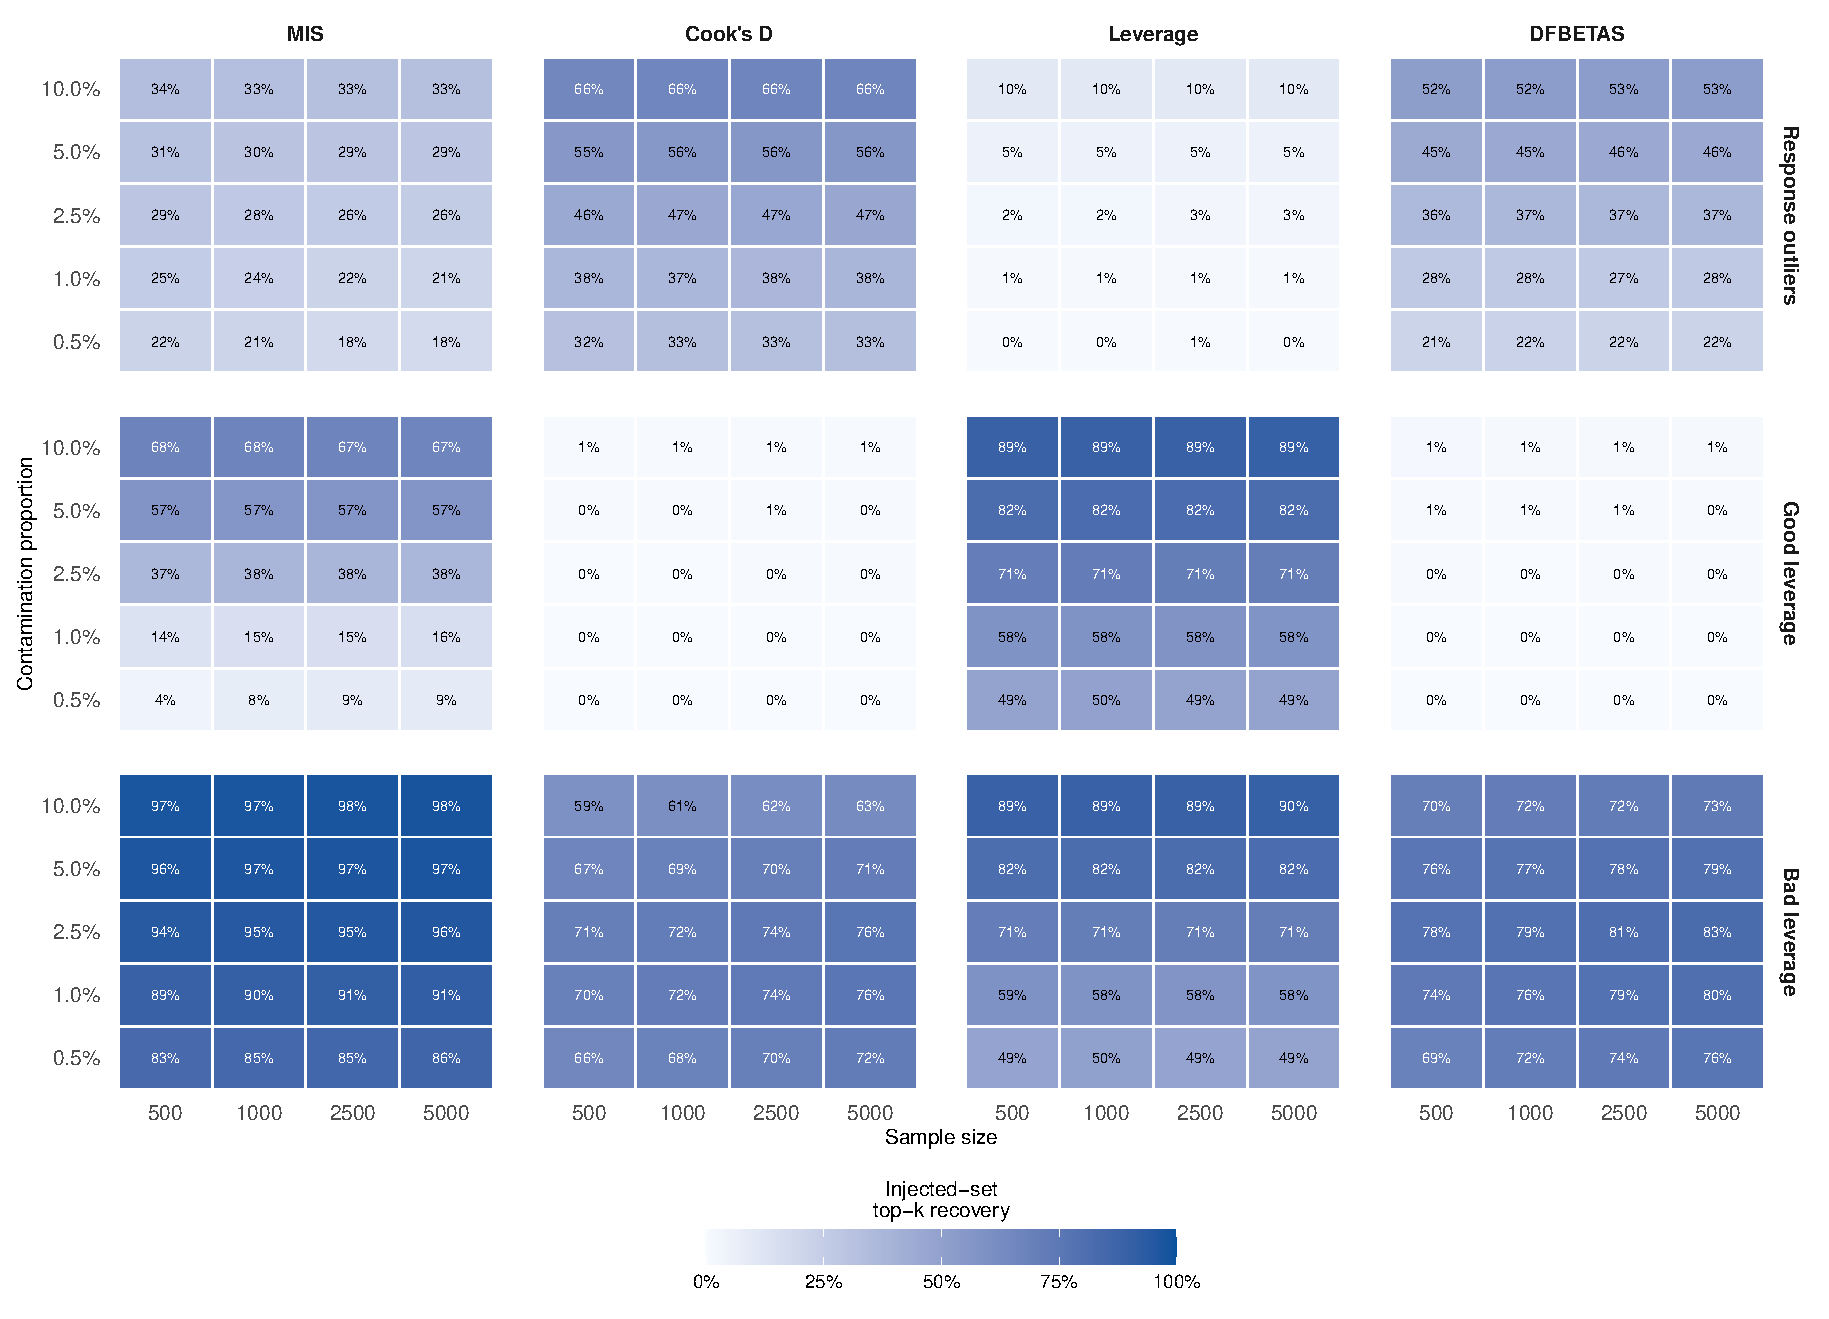
\includegraphics[width=\textwidth]{../../output/02_distributional/figures/supplement/02_figA1_all_method_overlap_heatmaps.pdf}
	\caption{Injected-set top-\(k\) recovery for MIS, Cook's distance, leverage, and DFBETAS across sample sizes, contamination proportions, and contamination mechanisms.}
	\label{fig:02A-all-method-overlap}
\end{figure}

\begin{table}[htbp]
\centering
\caption{Target-aware recovery difference, in percentage points, by sample size and contamination proportion. For bad leverage, positive values indicate greater recovery by MIS than the highest-recovery classical diagnostic. For vertical outliers and good leverage, positive values indicate lower unnecessary recovery by MIS than the lowest-recovery classical diagnostic.}
\label{tab:02A-mis-advantage-grid}
\resizebox{0.85\columnwidth}{!}{%
\begin{tabular}{@{}llrrr@{}}
\toprule
Sample size & Contamination & Response outliers & Good leverage & Bad leverage \\
\midrule
500 & 0.5\% & -- & -4.2 pp & +14.5 pp \\
500 & 1.0\% & -- & -13.6 pp & +15.0 pp \\
500 & 2.5\% & -- & -36.7 pp & +16.0 pp \\
500 & 5.0\% & -- & -57.1 pp & +14.4 pp \\
500 & 10.0\% & -- & -67.0 pp & +8.1 pp \\
1000 & 0.5\% & -- & -7.7 pp & +13.0 pp \\
1000 & 1.0\% & -- & -14.9 pp & +13.7 pp \\
1000 & 2.5\% & -- & -38.2 pp & +15.4 pp \\
1000 & 5.0\% & -- & -56.4 pp & +14.2 pp \\
1000 & 10.0\% & -- & -66.9 pp & +8.0 pp \\
2500 & 0.5\% & -- & -8.8 pp & +11.2 pp \\
2500 & 1.0\% & -- & -15.2 pp & +12.2 pp \\
2500 & 2.5\% & -- & -37.5 pp & +14.0 pp \\
2500 & 5.0\% & -- & -56.6 pp & +14.6 pp \\
2500 & 10.0\% & -- & -66.5 pp & +8.3 pp \\
5000 & 0.5\% & -- & -9.2 pp & +10.3 pp \\
5000 & 1.0\% & -- & -15.5 pp & +11.1 pp \\
5000 & 2.5\% & -- & -37.2 pp & +13.0 pp \\
5000 & 5.0\% & -- & -56.8 pp & +14.9 pp \\
5000 & 10.0\% & -- & -66.4 pp & +8.2 pp \\
\bottomrule
\end{tabular}%
}
\end{table}


Distribution-specific comparisons show that the bad-leverage result remains strong across most error distributions. MIS recovery exceeded \(97\%\) under normal, Beta\((2,5)\), mixed-normal, skewed-\(t\), and Pareto errors, with positive recovery differences relative to the highest-recovery classical diagnostic in every error distribution (\autoref{tab:02A-detection-by-error}). The largest differences occurred under GOLM and contaminated errors, at \(21.1\) and \(17.3\) percentage points. GPD errors produced the weakest separation: MIS recovered \(78.5\%\) of the injected bad-leverage observations and exceeded the classical benchmark by \(3.2\) percentage points. The distributional variation therefore qualifies the strength of the bad-leverage result without changing its direction.

\begin{figure}[htbp]
	\centering
	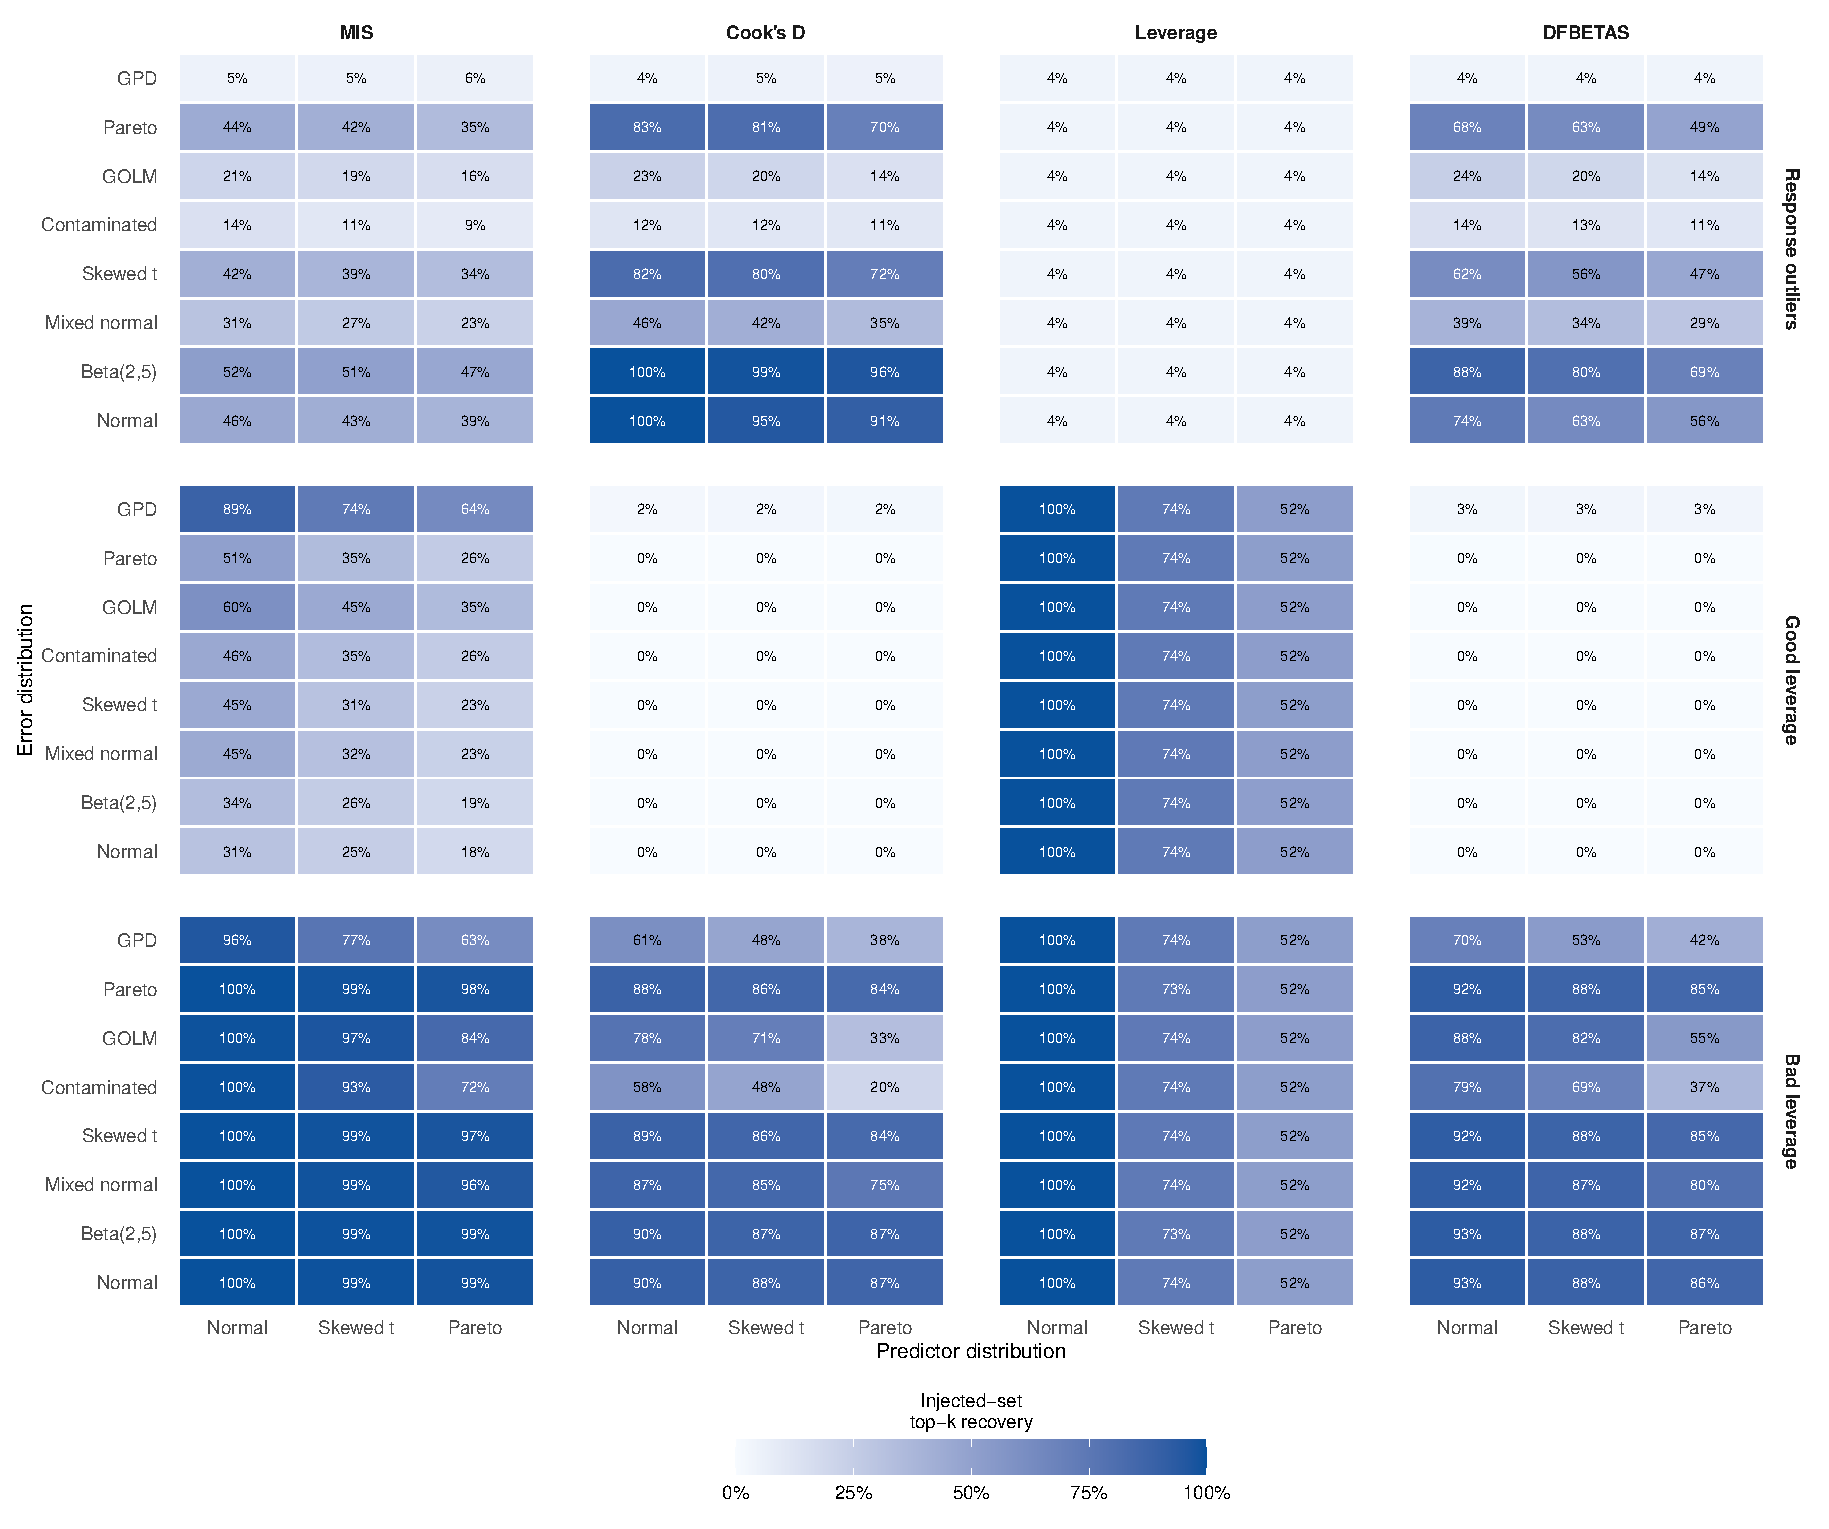
\includegraphics[width=\textwidth]{../../output/02_distributional/figures/supplement/02_figA1b_all_method_overlap_dgp_heatmaps.pdf}
	\caption{Injected-set top-\(k\) recovery for MIS, Cook's distance, leverage, and DFBETAS across predictor distributions, error distributions, and contamination mechanisms. Each cell averages over the remaining recorded design dimensions.}
	\label{fig:02A-all-method-overlap-dgp}
\end{figure}

\begin{table}[htbp]
\centering
\caption{Injected-set recovery and EVT convergence by error distribution and contamination mechanism.}
\label{tab:02A-detection-by-error}
\resizebox{\columnwidth}{!}{%
\begin{tabular}{@{}llrrrr@{}}
\toprule
Error distribution & Outlier mechanism & MIS recovery & Highest classical recovery & Recovery difference & EVT convergence \\
\midrule
Normal & Response outliers & 41.6\% & 93.7\% & -52.1 pp & 100.0\% \\
Normal & Good leverage & 22.6\% & 67.2\% & -44.5 pp & 100.0\% \\
Normal & Bad leverage & 99.1\% & 87.8\% & +11.3 pp & 100.0\% \\
Beta(2,5) & Response outliers & 49.1\% & 97.8\% & -48.8 pp & 100.0\% \\
Beta(2,5) & Good leverage & 23.7\% & 66.8\% & -43.1 pp & 100.0\% \\
Beta(2,5) & Bad leverage & 99.2\% & 88.0\% & +11.2 pp & 100.0\% \\
Mixed normal & Response outliers & 25.5\% & 39.6\% & -14.1 pp & 100.0\% \\
Mixed normal & Good leverage & 29.5\% & 67.1\% & -37.6 pp & 100.0\% \\
Mixed normal & Bad leverage & 97.6\% & 84.4\% & +13.2 pp & 100.0\% \\
Skewed t & Response outliers & 38.2\% & 78.0\% & -39.9 pp & 100.0\% \\
Skewed t & Good leverage & 33.1\% & 75.3\% & -42.2 pp & 100.0\% \\
Skewed t & Bad leverage & 98.8\% & 88.2\% & +10.6 pp & 100.0\% \\
Contaminated & Response outliers & 10.4\% & 12.5\% & -2.1 pp & 100.0\% \\
Contaminated & Good leverage & 32.0\% & 67.1\% & -35.1 pp & 100.0\% \\
Contaminated & Bad leverage & 84.4\% & 67.0\% & +17.3 pp & 100.0\% \\
GOLM & Response outliers & 17.7\% & 17.8\% & -0.1 pp & 100.0\% \\
GOLM & Good leverage & 42.5\% & 67.1\% & -24.6 pp & 100.0\% \\
GOLM & Bad leverage & 91.6\% & 70.5\% & +21.1 pp & 100.0\% \\
Pareto & Response outliers & 40.6\% & 78.0\% & -37.4 pp & 100.0\% \\
Pareto & Good leverage & 37.2\% & 75.2\% & -38.1 pp & 100.0\% \\
Pareto & Bad leverage & 98.8\% & 88.3\% & +10.5 pp & 100.0\% \\
GPD & Response outliers & 5.3\% & 4.7\% & +0.6 pp & 97.1\% \\
GPD & Good leverage & 75.3\% & 75.3\% & -0.0 pp & 97.3\% \\
GPD & Bad leverage & 78.5\% & 75.3\% & +3.2 pp & 97.4\% \\
\bottomrule
\end{tabular}%
}
\end{table}


\subsubsection{Good-Leverage Mechanism Diagnostics}
\label{app:good-leverage-diagnostics}

The summary mechanism comparison is reported in \autoref{fig:02-good-leverage-mechanism} and \autoref{tab:02-good-leverage-mechanism} in the main text. This diagnostic is a separate fixed-design exercise with \(n=1000\), \(k=10\), normal predictors, contamination magnitude \(10\), and \(200\) Monte Carlo iterations per error distribution. Because \(k=10\), iteration-level recovery changes in increments of ten percentage points. The analysis provides additional evidence for the same mechanism-specific interpretation. Across most error distributions, MIS-selected sets lie below the leverage-equality line and above the residual-equality line in \autoref{fig:02A-leverage-residual-scatter}. MIS therefore tends to substitute observations with lower leverage and larger residual magnitude for injected observations that are extreme in predictor space but approximately aligned with the fitted regression relation. Recovery increases when the injected observations themselves become more similar to the coefficient-influential sets selected by MIS, most visibly under GPD errors.

\begin{figure}[htbp]
	\centering
	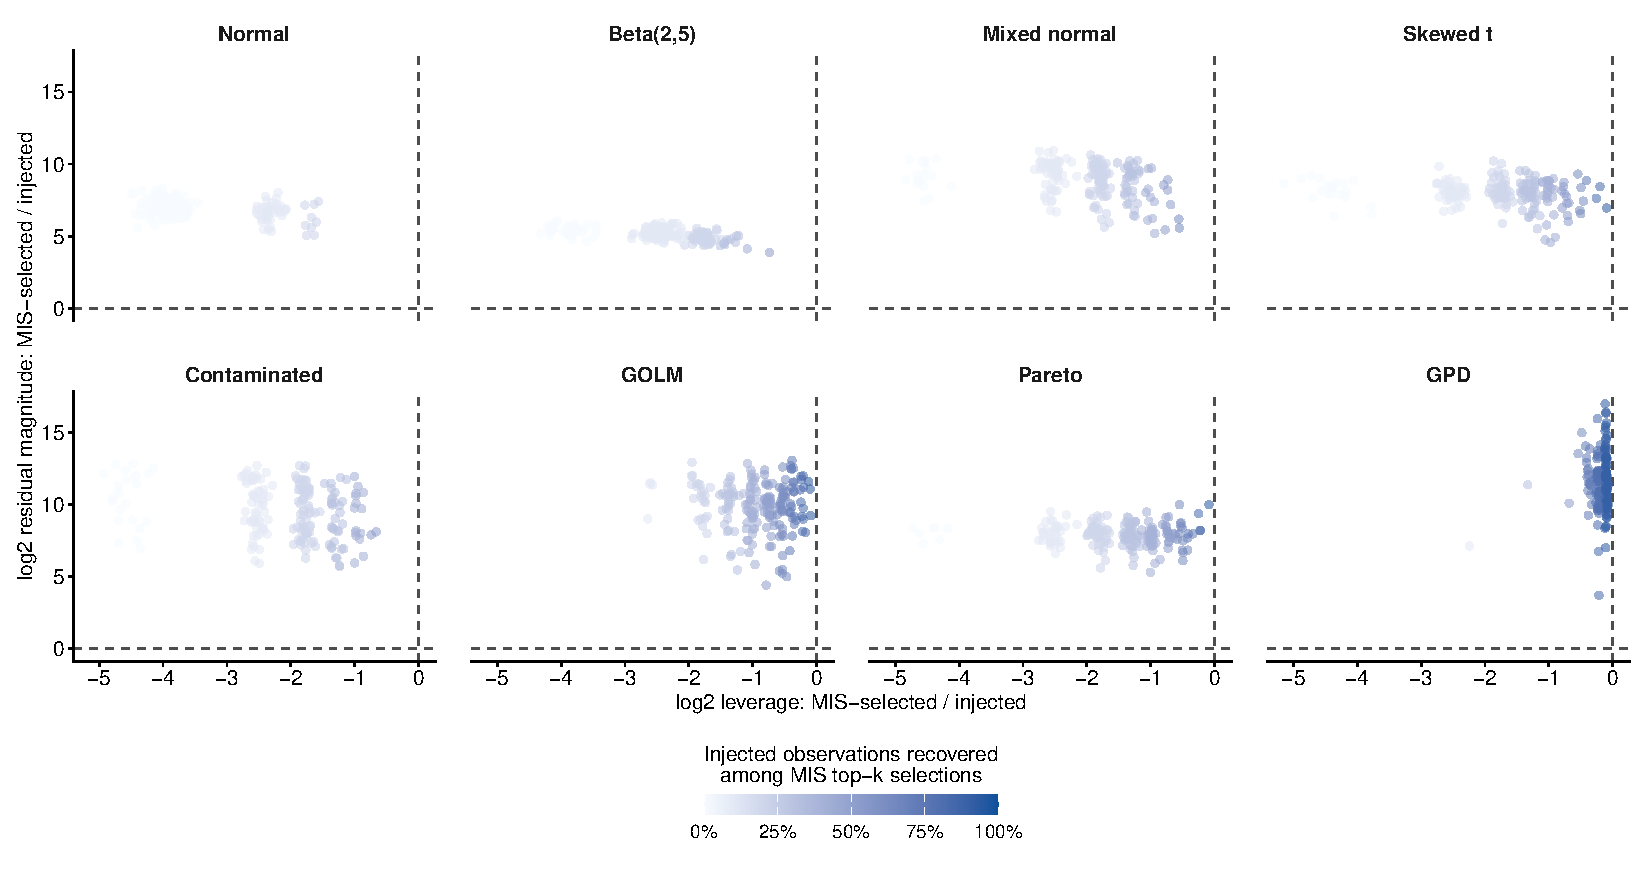
\includegraphics[width=\textwidth]{../../output/02_distributional/figures/supplement/02_figA3_leverage_residual_scatter.pdf}
	\caption{Iteration-level comparison of leverage and residual magnitude between the MIS-selected and injected good-leverage sets. The horizontal and vertical dashed lines denote equality, and shading indicates the proportion of injected observations recovered among the MIS top-\(k\) selections.}
	\label{fig:02A-leverage-residual-scatter}
\end{figure}

\subsubsection{EVT Convergence and Computational Diagnostics}
\label{app:detection-evt-diagnostics}

\begin{table}[htbp]
\centering
\caption{Uncontaminated MIS-EVT rejection and numerical convergence. Results are averaged with equal weight across the recorded design-cell summaries.}
\label{tab:02-empirical-size-summary}
\resizebox{0.7\columnwidth}{!}{%
\begin{tabular}{@{}lrrr@{}}
\toprule
Method & Empirical rejection & EVT convergence & Design cells \\
\midrule
MIS-EVT & 4.5\% & 99.7\% & 1980 \\
\bottomrule
\end{tabular}%
}
\end{table}


The uncontaminated MIS-EVT result reported in \autoref{tab:02-empirical-size-summary} is accompanied by high numerical convergence in the marginal sample-size and contamination summaries (\autoref{fig:02A-evt-convergence} and \autoref{tab:02A-evt-convergence-grid}). Distribution-specific convergence is somewhat lower in the GPD stress condition, so the marginal convergence range should not be read as a minimum over every recorded distributional cell. More importantly, convergence concerns only the numerical availability of the EVT rejection calculation. Injected-set recovery is computed before GEV fitting and therefore does not depend on EVT convergence.

\begin{figure}[htbp]
	\centering
	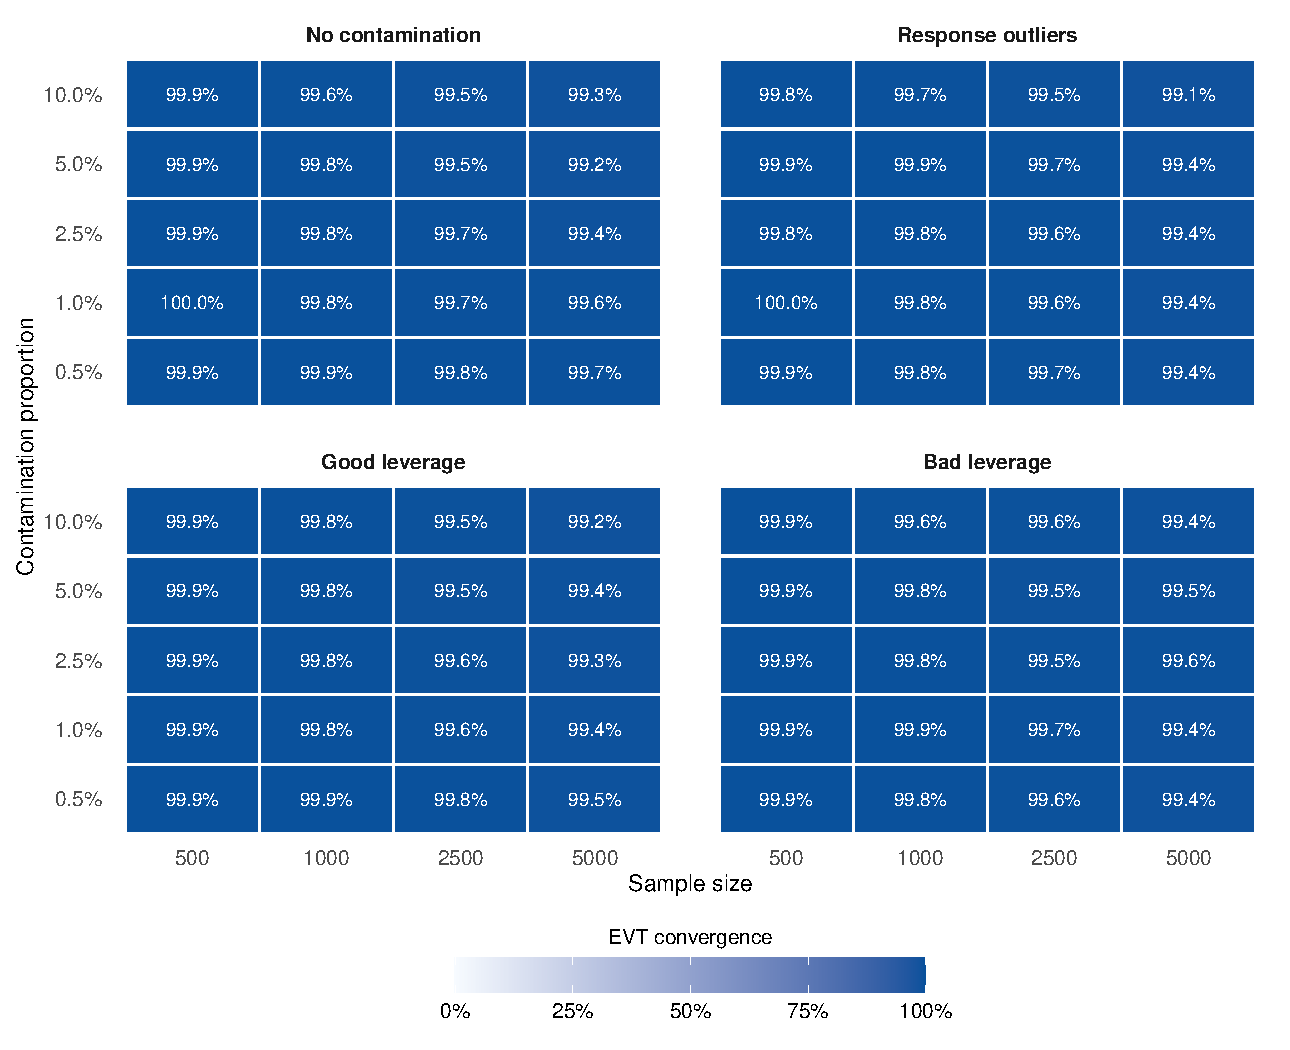
\includegraphics[width=0.95\textwidth]{../../output/02_distributional/figures/supplement/02_figA2_evt_convergence_heatmap.pdf}
	\caption{EVT convergence rates across sample sizes, contamination proportions, and contamination mechanisms.}
	\label{fig:02A-evt-convergence}
\end{figure}

\begin{table}[htbp]
\centering
\caption{EVT convergence rates by sample size, contamination proportion, and contamination mechanism.}
\label{tab:02A-evt-convergence-grid}
\resizebox{0.85\columnwidth}{!}{%
\begin{tabular}{@{}llrrrr@{}}
\toprule
Sample size & Contamination & No contamination & Response outliers & Good leverage & Bad leverage \\
\midrule
500 & 0.5\% & 99.9\% & 99.9\% & 99.9\% & 99.9\% \\
500 & 1.0\% & 100.0\% & 100.0\% & 99.9\% & 99.9\% \\
500 & 2.5\% & 99.9\% & 99.8\% & 99.9\% & 99.9\% \\
500 & 5.0\% & 99.9\% & 99.9\% & 99.9\% & 99.9\% \\
500 & 10.0\% & 99.9\% & 99.8\% & 99.9\% & 99.9\% \\
1000 & 0.5\% & 99.9\% & 99.8\% & 99.9\% & 99.8\% \\
1000 & 1.0\% & 99.8\% & 99.8\% & 99.8\% & 99.9\% \\
1000 & 2.5\% & 99.8\% & 99.8\% & 99.8\% & 99.8\% \\
1000 & 5.0\% & 99.8\% & 99.9\% & 99.8\% & 99.8\% \\
1000 & 10.0\% & 99.6\% & 99.7\% & 99.8\% & 99.6\% \\
2500 & 0.5\% & 99.8\% & 99.7\% & 99.8\% & 99.6\% \\
2500 & 1.0\% & 99.7\% & 99.6\% & 99.6\% & 99.7\% \\
2500 & 2.5\% & 99.7\% & 99.6\% & 99.6\% & 99.5\% \\
2500 & 5.0\% & 99.5\% & 99.7\% & 99.5\% & 99.5\% \\
2500 & 10.0\% & 99.5\% & 99.5\% & 99.5\% & 99.6\% \\
5000 & 0.5\% & 99.7\% & 99.4\% & 99.5\% & 99.4\% \\
5000 & 1.0\% & 99.6\% & 99.4\% & 99.4\% & 99.4\% \\
5000 & 2.5\% & 99.4\% & 99.4\% & 99.3\% & 99.6\% \\
5000 & 5.0\% & 99.2\% & 99.4\% & 99.4\% & 99.5\% \\
5000 & 10.0\% & 99.3\% & 99.1\% & 99.2\% & 99.4\% \\
\bottomrule
\end{tabular}%
}
\end{table}


The distribution-level GEV summaries show similar null rejection across most error distributions under the no-contamination scenario (\autoref{tab:02A-gev-summary}). Excluding the GPD stress condition, rejection rates ranged from \(4.0\%\) to \(5.3\%\). Under bad leverage, rejection exceeded \(94\%\) for every error distribution except GPD, where it fell to \(58.0\%\). Good-leverage rejection remained between \(1.0\%\) and \(3.4\%\), consistent with the limited target-coefficient disturbance generated by that mechanism. The GPD condition requires separate interpretation because the simulated shape parameters, \(\xi\in\{1.5,3,5,10\}\), imply an infinite population mean. Sample centring does not restore the usual finite-moment population conditions, so this condition is retained as an extreme stress test rather than treated as a regular sampling regime. Its GEV location and scale estimates should therefore not be compared directly with those from the finite-moment designs.

\begin{table}[htbp]
\centering
\caption{GEV convergence, rejection, parameter, and computation-time summaries by error distribution and scenario.}
\label{tab:02A-gev-summary}
\resizebox{\columnwidth}{!}{%
\begin{tabular}{@{}llrrrrrr@{}}
\toprule
Error distribution & Scenario & Convergence & Rejection & Median shape & Median scale & Median location & Median time (s) \\
\midrule
Normal & No contamination & 100.0\% & 4.5\% & 0.000 & 0.002 & 0.004 & 0.014 \\
Normal & Response outliers & 100.0\% & 71.8\% & 0.000 & 0.003 & 0.004 & 0.014 \\
Normal & Good leverage & 100.0\% & 1.1\% & 0.000 & 0.002 & 0.004 & 0.015 \\
Normal & Bad leverage & 100.0\% & 97.1\% & 0.060 & 0.015 & 0.023 & 0.014 \\
Beta(2,5) & No contamination & 100.0\% & 4.0\% & 0.000 & 0.000 & 0.001 & 0.016 \\
Beta(2,5) & Response outliers & 100.0\% & 81.3\% & 0.000 & 0.001 & 0.001 & 0.015 \\
Beta(2,5) & Good leverage & 100.0\% & 1.3\% & 0.000 & 0.000 & 0.001 & 0.016 \\
Beta(2,5) & Bad leverage & 100.0\% & 96.9\% & 0.093 & 0.015 & 0.019 & 0.015 \\
Mixed normal & No contamination & 100.0\% & 4.4\% & 0.231 & 0.006 & 0.008 & 0.014 \\
Mixed normal & Response outliers & 100.0\% & 45.7\% & 0.235 & 0.007 & 0.009 & 0.014 \\
Mixed normal & Good leverage & 100.0\% & 1.2\% & 0.227 & 0.006 & 0.008 & 0.015 \\
Mixed normal & Bad leverage & 100.0\% & 97.0\% & 0.221 & 0.022 & 0.035 & 0.014 \\
Skewed t & No contamination & 100.0\% & 4.2\% & 0.009 & 0.002 & 0.004 & 0.014 \\
Skewed t & Response outliers & 100.0\% & 66.3\% & 0.010 & 0.003 & 0.004 & 0.014 \\
Skewed t & Good leverage & 100.0\% & 1.4\% & 0.000 & 0.002 & 0.003 & 0.015 \\
Skewed t & Bad leverage & 100.0\% & 97.5\% & 0.010 & 0.017 & 0.033 & 0.014 \\
Contaminated & No contamination & 100.0\% & 4.4\% & 0.423 & 0.025 & 0.028 & 0.014 \\
Contaminated & Response outliers & 100.0\% & 11.3\% & 0.421 & 0.025 & 0.028 & 0.014 \\
Contaminated & Good leverage & 100.0\% & 1.0\% & 0.413 & 0.023 & 0.027 & 0.015 \\
Contaminated & Bad leverage & 100.0\% & 94.7\% & 0.371 & 0.045 & 0.065 & 0.014 \\
GOLM & No contamination & 100.0\% & 4.9\% & 0.438 & 0.011 & 0.016 & 0.014 \\
GOLM & Response outliers & 100.0\% & 15.3\% & 0.458 & 0.011 & 0.016 & 0.014 \\
GOLM & Good leverage & 100.0\% & 1.8\% & 0.402 & 0.011 & 0.016 & 0.015 \\
GOLM & Bad leverage & 100.0\% & 96.2\% & 0.407 & 0.030 & 0.042 & 0.014 \\
Pareto & No contamination & 100.0\% & 5.3\% & 0.000 & 0.001 & 0.001 & 0.015 \\
Pareto & Response outliers & 100.0\% & 69.2\% & 0.000 & 0.002 & 0.002 & 0.014 \\
Pareto & Good leverage & 100.0\% & 1.7\% & 0.000 & 0.001 & 0.001 & 0.015 \\
Pareto & Bad leverage & 100.0\% & 97.5\% & 0.010 & 0.017 & 0.033 & 0.014 \\
GPD & No contamination & 97.4\% & 4.2\% & 0.217 & 38097963.840 & 19507.658 & 0.015 \\
GPD & Response outliers & 97.1\% & 4.6\% & 0.216 & 37871306.492 & 15801.518 & 0.015 \\
GPD & Good leverage & 97.3\% & 3.4\% & 0.207 & 36524439.917 & 12081.373 & 0.016 \\
GPD & Bad leverage & 97.4\% & 58.0\% & 0.201 & 36314084.619 & 4978.303 & 0.015 \\
\bottomrule
\end{tabular}%
}
\end{table}


Adaptive block selection reduces the number of EVT blocks as the deletion set grows (\autoref{tab:02A-block-count-summary}). Fifty blocks were retained at contamination proportions of \(0.5\%\) and \(1\%\), while the median count declined to approximately \(39\)--\(40\) at \(2.5\%\), \(19\) at \(5\%\), and \(9\) at \(10\%\). Numerical convergence remained high even in the largest-contamination configurations, but convergence alone does not establish a well-supported GEV approximation. At the \(10\%\) deletion budget, the median block count is \(9\). Configurations with fewer than ten block maxima are treated as low-quality EVT configurations in the numerical diagnostics, so the corresponding rejection results should be interpreted cautiously.

\begin{table}[htbp]
\centering
\caption{Block-maxima configuration by sample size and contamination proportion. Block size is computed after removing the size-k reference set, and the final column reports the ratio of the deletion budget to block size.}
\label{tab:02A-block-count-summary}
\resizebox{0.85\columnwidth}{!}{%
\begin{tabular}{@{}lrrrrr@{}}
\toprule
Sample size & Contamination & Set size & Blocks & Block size & k / block size \\
\midrule
500 & 0.5\% & 2 & 50 & 9 & 0.22 \\
500 & 1.0\% & 5 & 50 & 9 & 0.56 \\
500 & 2.5\% & 12 & 40 & 12 & 1.00 \\
500 & 5.0\% & 25 & 19 & 25 & 1.00 \\
500 & 10.0\% & 50 & 9 & 50 & 1.00 \\
1000 & 0.5\% & 5 & 50 & 19 & 0.26 \\
1000 & 1.0\% & 10 & 50 & 19 & 0.53 \\
1000 & 2.5\% & 25 & 39 & 25 & 1.00 \\
1000 & 5.0\% & 50 & 19 & 50 & 1.00 \\
1000 & 10.0\% & 100 & 9 & 100 & 1.00 \\
2500 & 0.5\% & 12 & 50 & 49 & 0.24 \\
2500 & 1.0\% & 25 & 50 & 49 & 0.51 \\
2500 & 2.5\% & 62 & 39 & 62 & 1.00 \\
2500 & 5.0\% & 125 & 19 & 125 & 1.00 \\
2500 & 10.0\% & 250 & 9 & 250 & 1.00 \\
5000 & 0.5\% & 25 & 50 & 99 & 0.25 \\
5000 & 1.0\% & 50 & 50 & 99 & 0.51 \\
5000 & 2.5\% & 125 & 39 & 125 & 1.00 \\
5000 & 5.0\% & 250 & 19 & 250 & 1.00 \\
5000 & 10.0\% & 500 & 9 & 500 & 1.00 \\
\bottomrule
\end{tabular}%
}
\end{table}


\subsection{Algorithmic and EVT Validation}
\label{app:numerical}

The algorithmic validation study evaluates the computational components underlying fixed-\(k\) MIS rather than supplying a separate substantive simulation result. The study compares greedy and Dinkelbach-based searches, with and without refinement, across linear, interaction, difficult, and partially linear regression architectures. It also compares alternative GEV fitting configurations for the EVT step. The purpose is to assess influence capture, injected-set overlap, computational scaling, set stability, numerical convergence, and null behaviour before these components are used in the substantive simulation studies.

\subsubsection{Search Accuracy and Influence Capture}
\label{app:03-search}

The Dinkelbach and greedy procedures should be compared using both injected-set overlap and attained influence. These quantities answer different questions. Injected-set overlap measures recovery of the observations used to construct the simulation disturbance, whereas the influence ratio compares the absolute DFBETA of the detected set with that of the injected set. A value near one therefore indicates that the detected set captures approximately the same coefficient influence even when its membership differs from the injected coalition.

Across the complete algorithmic design, refinement substantially increased injected-set overlap for both search procedures (\autoref{fig:03-detection-overlap} and \autoref{tab:03-algorithm-summary}). Mean overlap increased from \(77.1\%\) to \(96.5\%\) for greedy search and from \(80.4\%\) to \(94.1\%\) for the Dinkelbach-based search. More importantly for the optimisation objective, both refined procedures had a median influence ratio of \(1.00\), with 10th and 90th percentiles also equal to \(1.00\). Thus, differences in recovered membership do not generally imply differences of the same magnitude in coefficient influence.

\begin{figure}[htbp]
	\centering
	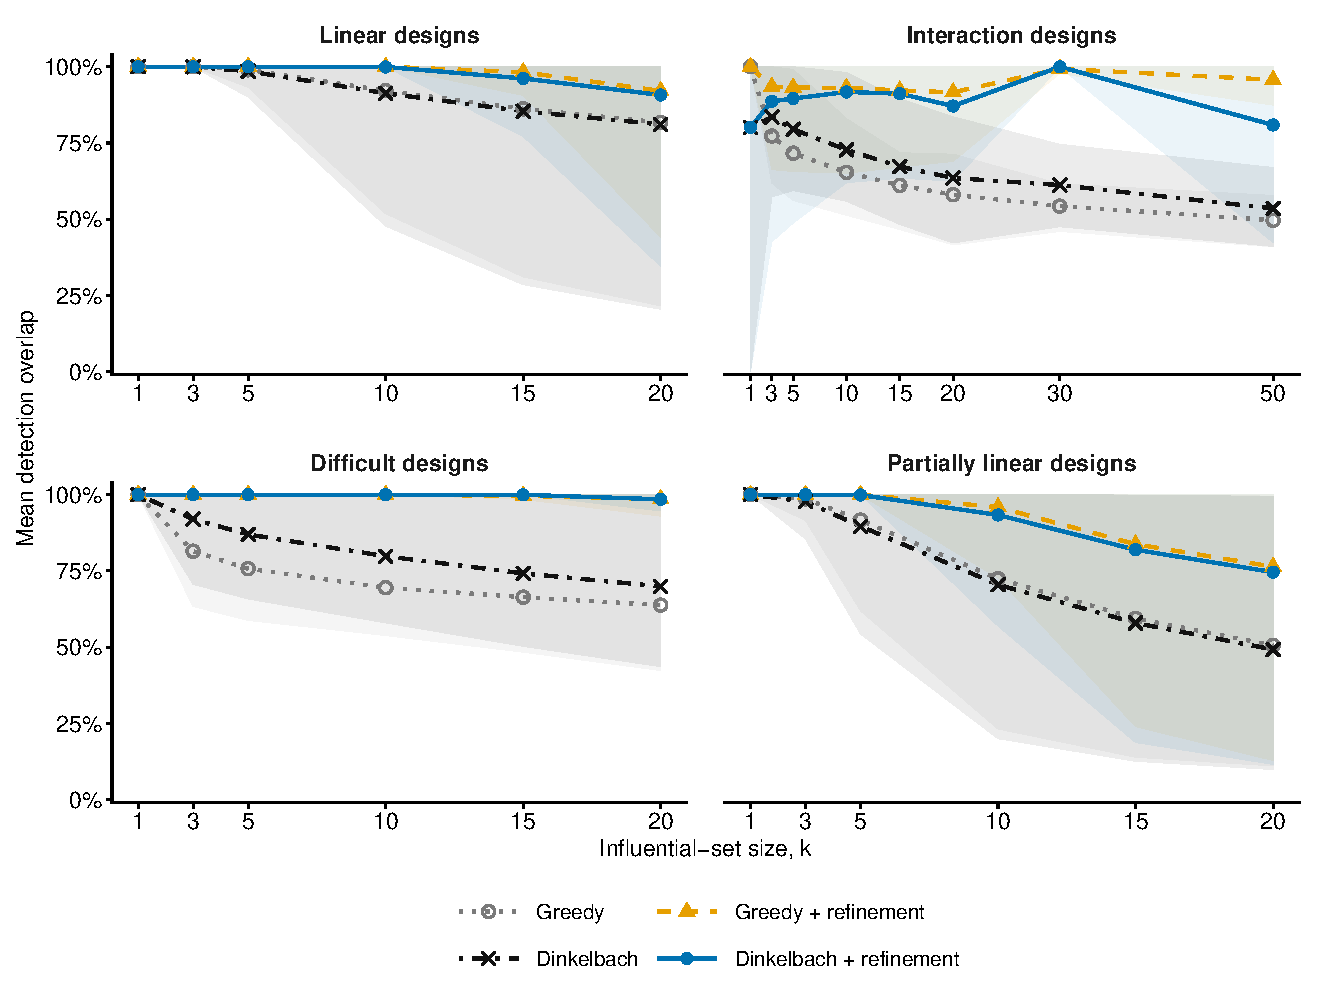
\includegraphics[width=\textwidth]{../../output/03_algorithmic/figures/main/03_fig1_detection_overlap.pdf}
	\caption{Mean injected-set overlap for greedy and Dinkelbach-based search, with and without refinement, across influential-set sizes and architecture groups.}
	\label{fig:03-detection-overlap}
\end{figure}

\begin{table}[htbp]
\centering
\caption{Detection accuracy, captured influence, and runtime across algorithmic design cells. Brackets report the indicated between-cell percentiles.}
\label{tab:03-algorithm-summary}
\resizebox{0.85\columnwidth}{!}{%
\begin{tabular}{@{}lrrr@{}}
\toprule
Detection method & Overlap, mean [P10, P90] & Influence ratio, median [P10, P90] & Runtime, median [IQR] (s) \\
\midrule
Greedy & 77.1\% [49.4, 100.0] & 1.00 [1.00, 4.20] & 0.0030 [0.0010, 0.0080] \\
Greedy + refinement & 96.5\% [92.5, 100.0] & 1.00 [1.00, 1.00] & 0.0080 [0.0040, 0.0485] \\
Dinkelbach & 80.4\% [48.6, 100.0] & 1.00 [1.00, 4.70] & 0.0020 [0.0010, 0.0040] \\
Dinkelbach + refinement & 94.1\% [80.0, 100.0] & 1.00 [1.00, 1.00] & 0.0050 [0.0040, 0.0170] \\
\bottomrule
\end{tabular}%
}
\end{table}


Architecture-specific results show why overlap should not be treated as the optimisation criterion. The refined Dinkelbach and refined greedy procedures both attain an influence ratio of \(1.00\) in every architecture-level summary, while their recovered memberships can differ (\autoref{tab:03A-architecture-comparison}). The largest discrepancy occurs in the triple-interaction architecture, where mean injected-set overlap is \(72.7\%\) for refined greedy search and \(48.4\%\) for refined Dinkelbach search. The Dinkelbach procedure nevertheless attains the same reported influence ratio. This distinction is consistent with the possibility that more than one size-\(k\) set can exert similar target-coefficient influence.

\begin{table}[htbp]
\centering
\small
\caption{Architecture-level comparison of the refined greedy and refined Dinkelbach detection methods.}
\label{tab:03A-architecture-comparison}
\resizebox{\columnwidth}{!}{%
\begin{tabular}{@{}lrrrrrr@{}}
\toprule
Architecture & Greedy-refined overlap & Dinkelbach-refined overlap & Dinkelbach advantage & Greedy-refined influence ratio & Dinkelbach-refined influence ratio & Dinkelbach/greedy runtime \\
\midrule
Simple linear & 100.0\% & 100.0\% & +0.0 pp & 1.00 & 1.00 & 1.00 \\
Complex linear & 96.8\% & 95.6\% & -1.2 pp & 1.00 & 1.00 & 0.22 \\
Interaction & 99.0\% & 96.8\% & -2.2 pp & 1.00 & 1.00 & 1.05 \\
Triple interaction & 72.7\% & 48.4\% & -24.2 pp & 1.00 & 1.00 & 0.17 \\
Sparse binary interaction & 100.0\% & 100.0\% & +0.0 pp & 1.00 & 1.00 & 0.89 \\
Polynomial interaction & 98.4\% & 95.4\% & -3.0 pp & 1.00 & 1.00 & 0.23 \\
High-k interaction & 99.2\% & 97.8\% & -1.3 pp & 1.00 & 1.00 & 1.20 \\
Nonlinear nuisance & 100.0\% & 100.0\% & +0.0 pp & 1.00 & 1.00 & 1.00 \\
Collinear interaction & 99.6\% & 99.7\% & +0.1 pp & 1.00 & 1.00 & 1.00 \\
PLM: confounded & 90.8\% & 89.2\% & -1.5 pp & 1.00 & 1.00 & 0.17 \\
PLM: nonlinear & 94.6\% & 94.0\% & -0.5 pp & 1.00 & 1.00 & 0.19 \\
\bottomrule
\end{tabular}%
}
\end{table}


The cell-level comparison gives the same qualification (\autoref{fig:03A-exact-refined-advantage}). Dinkelbach and greedy refinement agree closely over most architectures and set sizes, but membership differences appear in several interaction designs. The most pronounced discrepancy occurs for the triple-interaction design at small \(k\). These cells do not contradict the global-maximisation property of the Dinkelbach formulation: they show that correspondence with a planted set and maximisation of the fixed-residualised coefficient-influence objective are different evaluation criteria.

\begin{figure}[htbp]
	\centering
	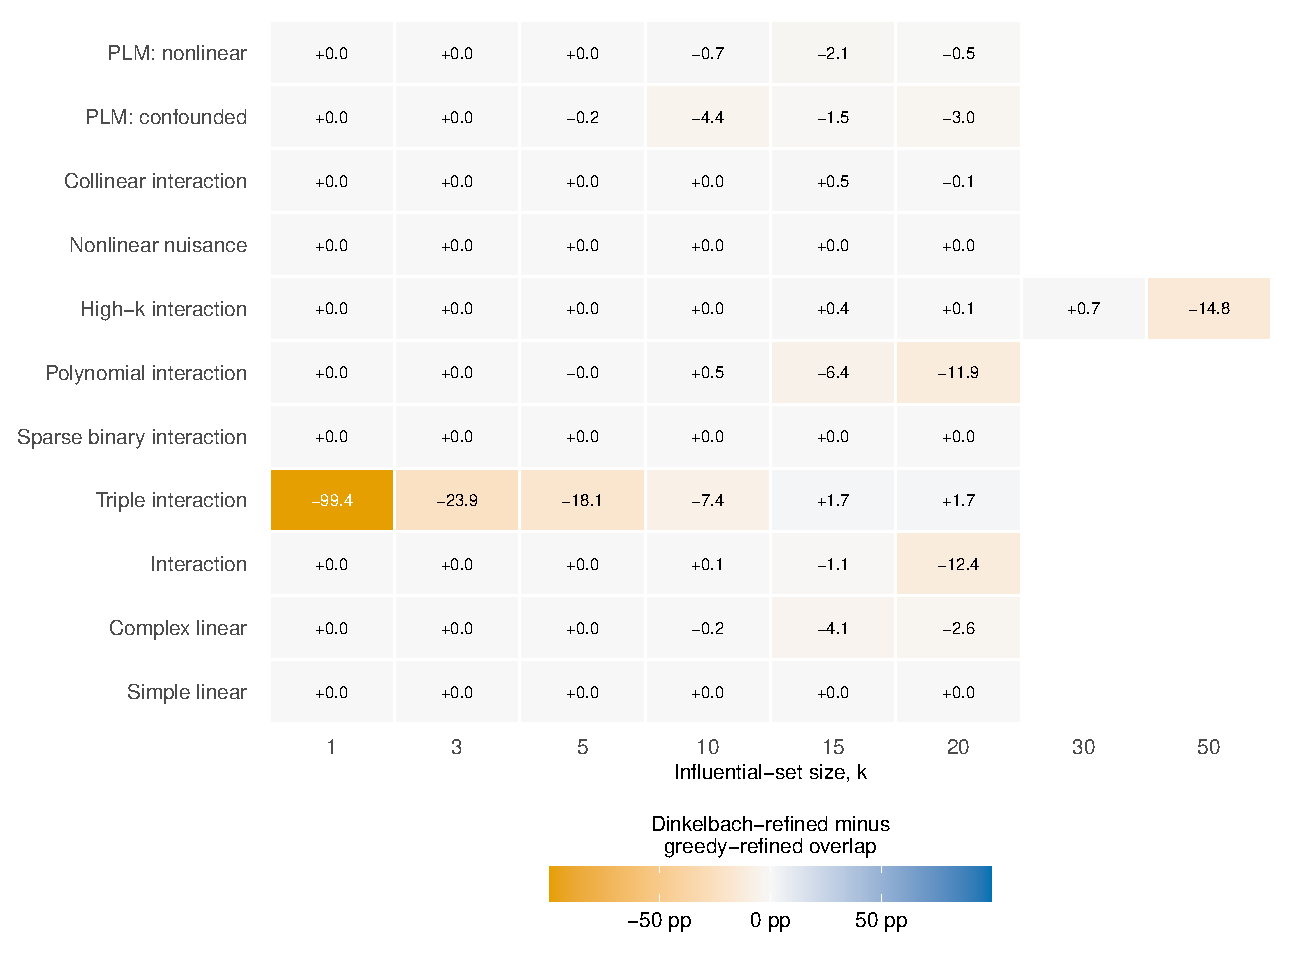
\includegraphics[width=\textwidth]{../../output/03_algorithmic/figures/supplement/03_figA2_exact_refined_advantage_heatmap.pdf}
	\caption{Difference in injected-set overlap between refined Dinkelbach and refined greedy search across architectures and influential-set sizes.}
	\label{fig:03A-exact-refined-advantage}
\end{figure}

The collinearity sensitivity exercise shows that these membership differences are concentrated in the smallest sample and largest set sizes (\autoref{fig:03A-collinearity}). At \(n\geq1000\), the overlap differences between refined Dinkelbach and refined greedy search are essentially zero throughout the displayed correlation grid. The comparison therefore provides no evidence that increasing predictor correlation systematically separates the two refined procedures in the larger designs.

\begin{figure}[htbp]
	\centering
	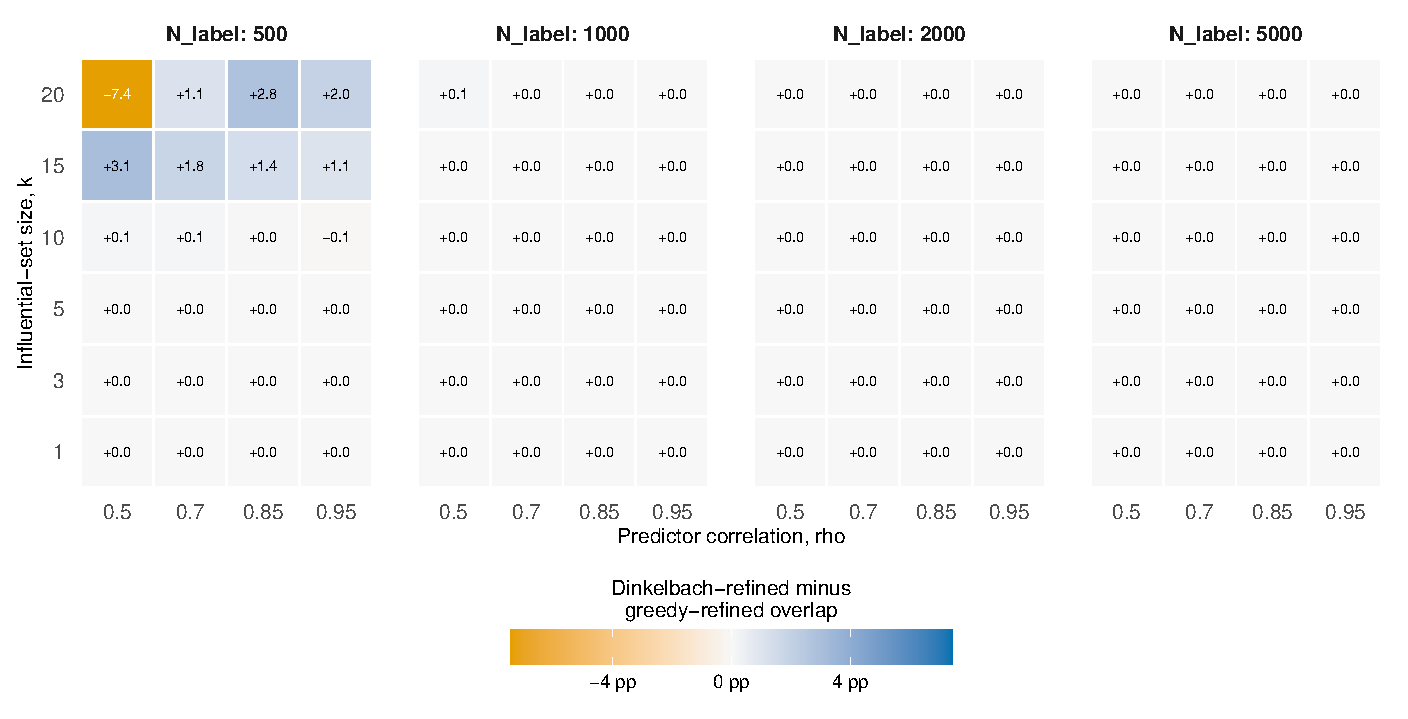
\includegraphics[width=\textwidth]{../../output/03_algorithmic/figures/supplement/03_figA6_collinearity_sensitivity.pdf}
	\caption{Difference in injected-set overlap between refined Dinkelbach and refined greedy search across predictor correlation, sample size, and influential-set size.}
	\label{fig:03A-collinearity}
\end{figure}


\subsubsection{Computational Scaling and Set Stability}
\label{app:03-computation}

Dinkelbach-based search remained computationally inexpensive over the recorded sample-size range. The unrefined Dinkelbach procedure had a median runtime of \(0.002\) seconds, compared with \(0.003\) seconds for unrefined greedy search, while Dinkelbach plus refinement required \(0.005\) seconds compared with \(0.008\) seconds for greedy plus refinement (\autoref{tab:03-algorithm-summary}). Runtime rises with sample size for all four procedures, but remains on the order of hundredths of a second at \(n=5000\) in the median comparison (\autoref{fig:03-detection-runtime}). The Dinkelbach formulation therefore does not introduce a prohibitive computational penalty in these designs.

\begin{figure}[htbp]
	\centering
	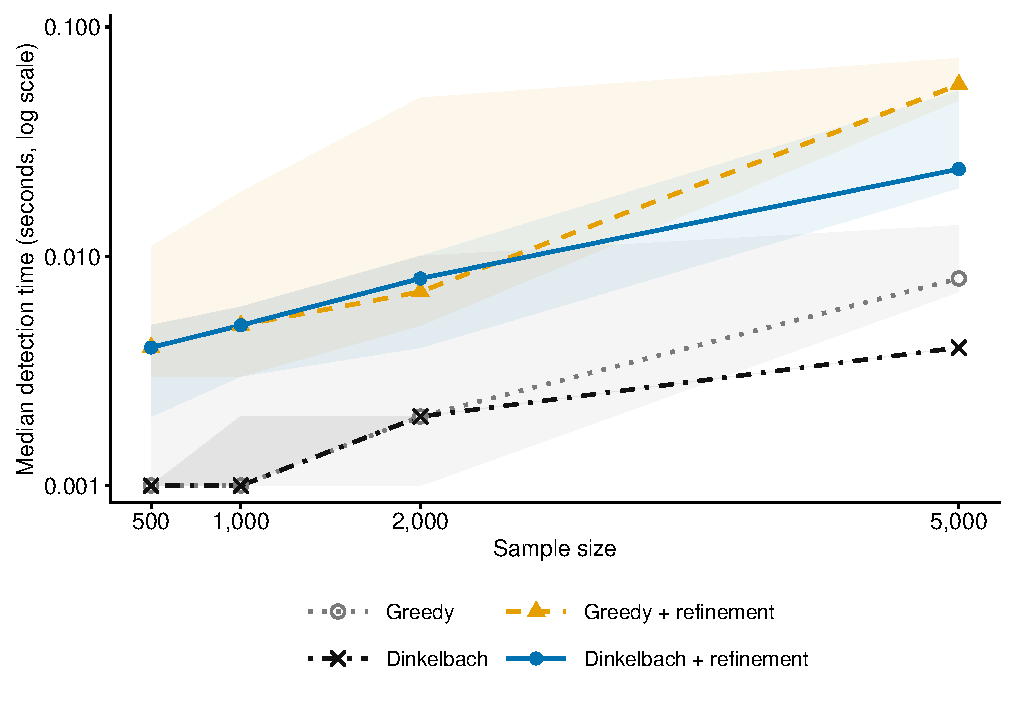
\includegraphics[width=0.82\textwidth]{../../output/03_algorithmic/figures/main/03_fig2a_detection_runtime.pdf}
	\caption{Median search runtime by sample size for greedy and Dinkelbach-based detection, with and without refinement.}
	\label{fig:03-detection-runtime}
\end{figure}

The nestedness traces provide a separate measure of set stability as \(k\) changes (\autoref{fig:03A-nestedness} and \autoref{tab:03A-nestedness-summary}). In the representative traces, the unrefined Dinkelbach procedure records no nestedness violations and a mean Jaccard similarity of \(0.863\) in each displayed architecture. Refinement can alter this path: for example, the refined Dinkelbach trace in the collinear-interaction design records five violations and a minimum successive-set Jaccard similarity of \(0.222\). Optimising the objective separately at each fixed \(k\) therefore does not imply that the resulting sequence of maximising sets must itself be nested across \(k\).

\begin{figure}[htbp]
	\centering
	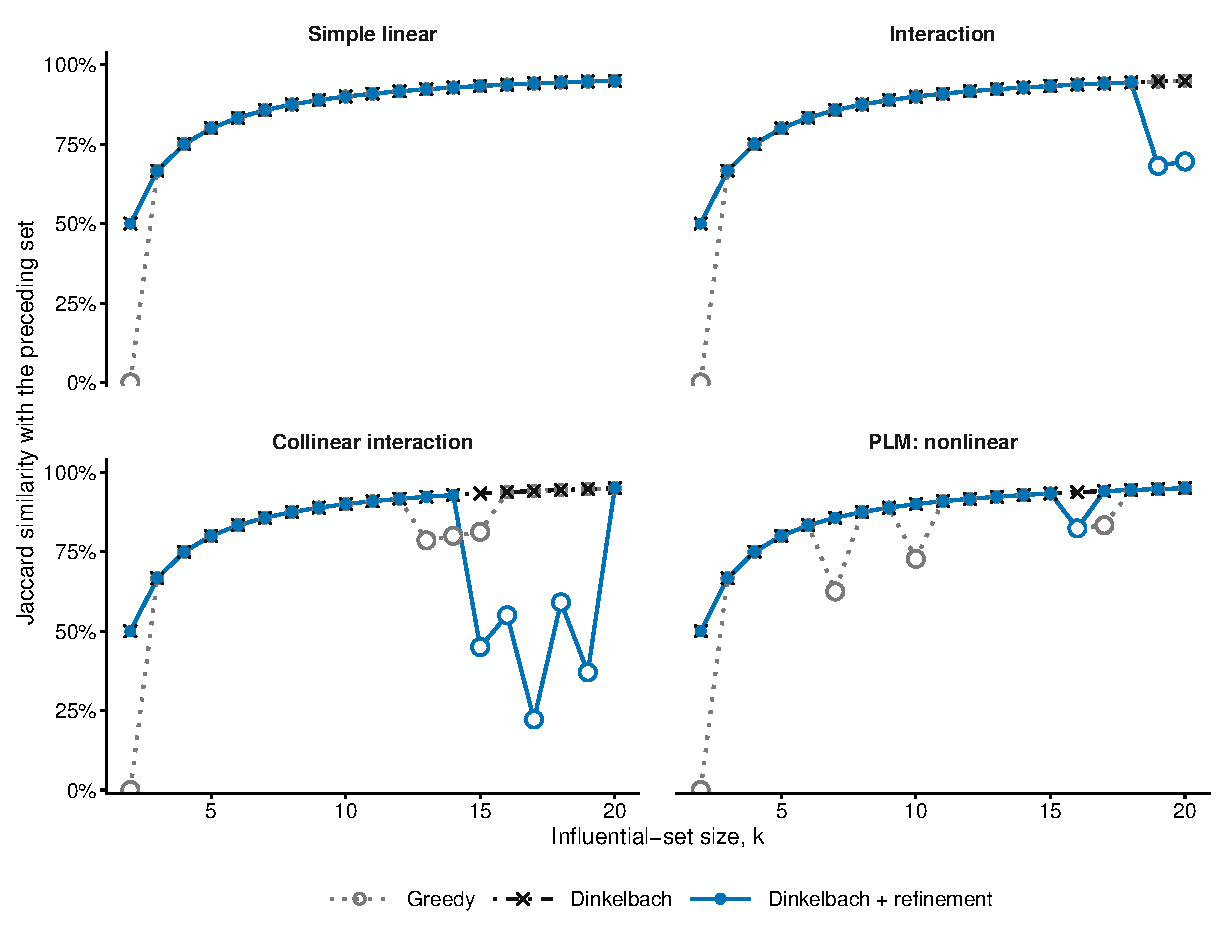
\includegraphics[width=\textwidth]{../../output/03_algorithmic/figures/supplement/03_figA4_nestedness_traces.pdf}
	\caption{Jaccard similarity between the size-\(k\) selected set and the preceding size-\((k-1)\) set for representative architectures.}
	\label{fig:03A-nestedness}
\end{figure}

\begin{table}[htbp]
\centering
\caption{Nestedness and computational summaries for the representative traces.}
\label{tab:03A-nestedness-summary}
\resizebox{\columnwidth}{!}{%
\begin{tabular}{@{}llrrrrr@{}}
\toprule
Architecture & Method & Mean Jaccard & Minimum Jaccard & Violations & Median time (s) & Final influence \\
\midrule
Simple linear & Dinkelbach & 0.863 & 0.500 & 0 & 0.0010 & 0.104 \\
Simple linear & Dinkelbach + refinement & 0.863 & 0.500 & 0 & 0.0020 & 0.104 \\
Simple linear & Greedy & 0.837 & 0.000 & 1 & 0.0030 & 0.104 \\
Interaction & Dinkelbach & 0.863 & 0.500 & 0 & 0.0010 & 0.018 \\
Interaction & Dinkelbach + refinement & 0.836 & 0.500 & 2 & 0.0020 & 0.010 \\
Interaction & Greedy & 0.837 & 0.000 & 1 & 0.0040 & 0.012 \\
Collinear interaction & Dinkelbach & 0.863 & 0.500 & 0 & 0.0010 & 0.020 \\
Collinear interaction & Dinkelbach + refinement & 0.731 & 0.222 & 5 & 0.0030 & 0.001 \\
Collinear interaction & Greedy & 0.817 & 0.000 & 4 & 0.0030 & 0.001 \\
PLM: nonlinear & Dinkelbach & 0.863 & 0.500 & 0 & 0.0010 & 0.124 \\
PLM: nonlinear & Dinkelbach + refinement & 0.857 & 0.500 & 1 & 0.0025 & 0.119 \\
PLM: nonlinear & Greedy & 0.804 & 0.000 & 5 & 0.0050 & 0.119 \\
\bottomrule
\end{tabular}%
}
\end{table}



\subsubsection{EVT Configuration and Numerical Convergence}
\label{app:03-evt}

The EVT comparison evaluates three computational configurations: greedy search with constrained GEV fitting, Dinkelbach-based search with constrained GEV fitting, and Dinkelbach-based search with the robust GEV fit. Under the contaminated algorithmic designs, the two Dinkelbach-based configurations achieve higher average signal rejection than the greedy-constrained configuration, while the robust GEV fit substantially improves numerical availability (\autoref{tab:03-evt-configuration-summary}). Mean convergence is \(94.3\%\) for greedy plus constrained GEV, \(94.8\%\) for Dinkelbach plus constrained GEV, and \(99.4\%\) for Dinkelbach plus robust GEV. Their mean rejection rates at the nominal \(5\%\) threshold in the contaminated designs are \(85.7\%\), \(92.4\%\), and \(91.9\%\), respectively.

\begin{table}[htbp]
\centering
\caption{EVT convergence, signal rejection, fitted shape, and runtime under the contaminated algorithmic simulations.}
\label{tab:03-evt-configuration-summary}
\resizebox{\columnwidth}{!}{%
\begin{tabular}{@{}lrrrr@{}}
\toprule
EVT configuration & Convergence, mean [P10, P90] & Rejection at 5\%, mean [P10, P90] & Shape, median [IQR] & Runtime, median [IQR] (s) \\
\midrule
Greedy + constrained GEV & 94.3\% [78.0, 100.0] & 85.7\% [41.0, 100.0] & 0.000 [-0.000, 0.000] & 0.0150 [0.0080, 0.0260] \\
Dinkelbach + constrained GEV & 94.8\% [80.0, 100.0] & 92.4\% [72.9, 100.0] & 0.000 [-0.000, 0.000] & 0.0080 [0.0060, 0.0090] \\
Dinkelbach + robust GEV & 99.4\% [100.0, 100.0] & 91.9\% [73.0, 100.0] & -0.000 [-0.000, 0.000] & 0.0075 [0.0060, 0.0100] \\
\bottomrule
\end{tabular}%
}
\end{table}


EVT runtime remains small relative to the broader simulation exercise (\autoref{fig:03-evt-runtime}). Median runtime is \(0.0150\) seconds for greedy plus constrained GEV, \(0.0080\) seconds for Dinkelbach plus constrained GEV, and \(0.0075\) seconds for Dinkelbach plus robust GEV. The Dinkelbach plus robust GEV configuration therefore combines the highest overall convergence with runtime comparable to, or below, the other recorded EVT configurations.

\begin{figure}[htbp]
	\centering
	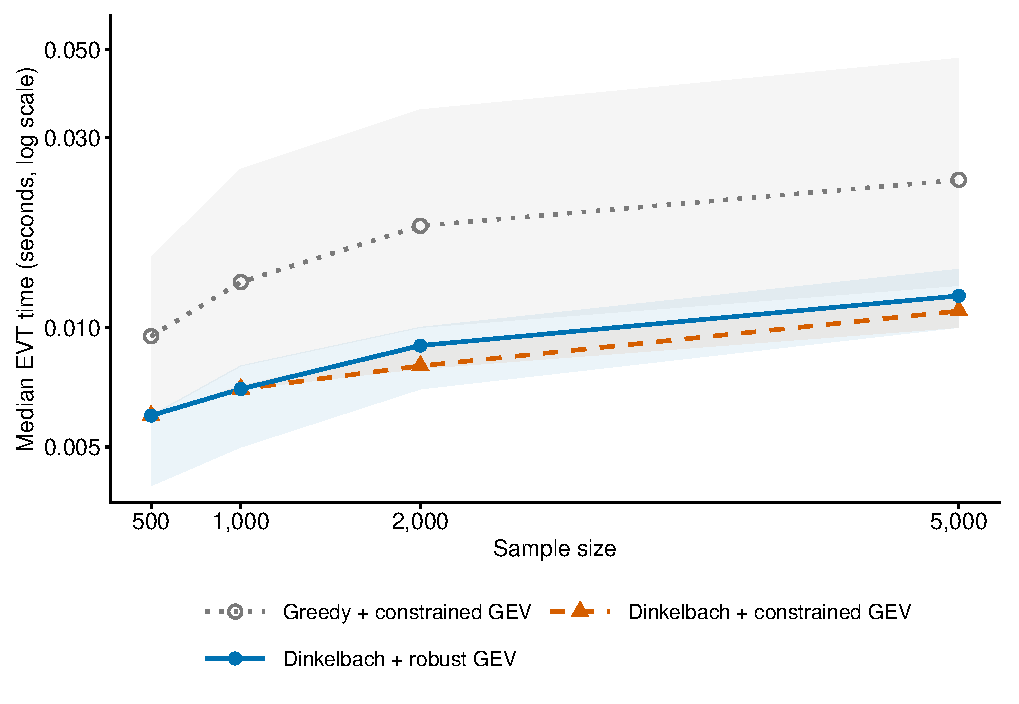
\includegraphics[width=0.82\textwidth]{../../output/03_algorithmic/figures/main/03_fig2b_evt_runtime.pdf}
	\caption{Median EVT runtime by sample size and fitting configuration.}
	\label{fig:03-evt-runtime}
\end{figure}

The architecture-level results show that the convergence improvement is broad but not literally universal (\autoref{fig:03A-evt-convergence} and \autoref{tab:03A-evt-by-architecture}). Dinkelbach plus robust GEV attains \(100\%\) convergence throughout most architecture--sample-size cells. The principal exception is the high-\(k\) interaction design, where convergence falls below \(100\%\) at several sample sizes. The robust fitting modification therefore substantially improves numerical reliability without eliminating every difficult configuration.

\begin{figure}[htbp]
	\centering
	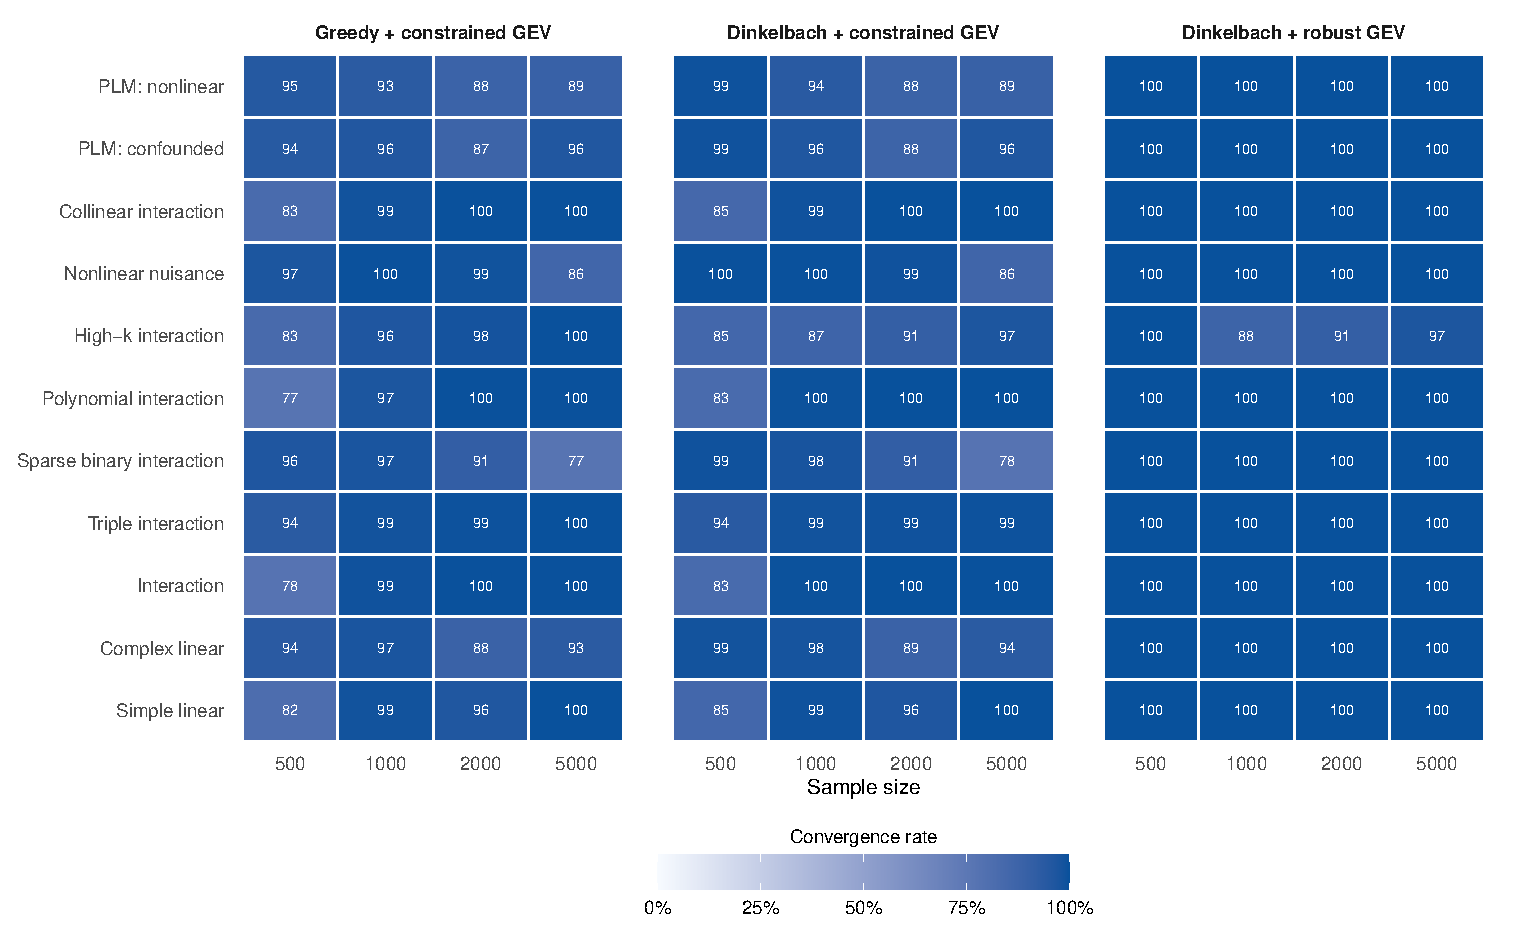
\includegraphics[width=\textwidth]{../../output/03_algorithmic/figures/supplement/03_figA7_evt_convergence_heatmap.pdf}
	\caption{EVT convergence rates by architecture, sample size, and search/fitting configuration.}
	\label{fig:03A-evt-convergence}
\end{figure}

\begin{table}[htbp]
\centering
\small
\caption{EVT performance by architecture and fitting configuration.}
\label{tab:03A-evt-by-architecture}
\resizebox{\columnwidth}{!}{%
\begin{tabular}{@{}llrrrr@{}}
\toprule
Architecture & EVT configuration & Convergence & Rejection at 5\% & Median shape & Median runtime (s) \\
\midrule
Simple linear & Greedy + constrained GEV & 94.1\% & 100.0\% & 0.000 & 0.0140 \\
Simple linear & Dinkelbach + constrained GEV & 95.2\% & 100.0\% & 0.000 & 0.0070 \\
Simple linear & Dinkelbach + robust GEV & 100.0\% & 99.6\% & -0.000 & 0.0070 \\
Complex linear & Greedy + constrained GEV & 93.2\% & 96.5\% & 0.000 & 0.0170 \\
Complex linear & Dinkelbach + constrained GEV & 94.8\% & 99.6\% & 0.000 & 0.0090 \\
Complex linear & Dinkelbach + robust GEV & 100.0\% & 99.5\% & -0.000 & 0.0070 \\
Interaction & Greedy + constrained GEV & 94.1\% & 74.2\% & 0.000 & 0.0145 \\
Interaction & Dinkelbach + constrained GEV & 95.7\% & 83.9\% & 0.000 & 0.0070 \\
Interaction & Dinkelbach + robust GEV & 100.0\% & 83.4\% & -0.000 & 0.0080 \\
Triple interaction & Greedy + constrained GEV & 97.9\% & 79.9\% & 0.000 & 0.0150 \\
Triple interaction & Dinkelbach + constrained GEV & 97.8\% & 91.9\% & 0.000 & 0.0080 \\
Triple interaction & Dinkelbach + robust GEV & 100.0\% & 92.1\% & 0.000 & 0.0080 \\
Sparse binary interaction & Greedy + constrained GEV & 90.5\% & 92.5\% & 0.000 & 0.0150 \\
Sparse binary interaction & Dinkelbach + constrained GEV & 91.4\% & 96.5\% & 0.000 & 0.0080 \\
Sparse binary interaction & Dinkelbach + robust GEV & 100.0\% & 96.7\% & -0.000 & 0.0060 \\
Polynomial interaction & Greedy + constrained GEV & 93.4\% & 73.6\% & 0.000 & 0.0145 \\
Polynomial interaction & Dinkelbach + constrained GEV & 95.6\% & 84.0\% & 0.000 & 0.0070 \\
Polynomial interaction & Dinkelbach + robust GEV & 100.0\% & 83.5\% & -0.000 & 0.0080 \\
High-k interaction & Greedy + constrained GEV & 95.2\% & 78.7\% & 0.000 & 0.0190 \\
High-k interaction & Dinkelbach + constrained GEV & 90.3\% & 88.3\% & 0.000 & 0.0070 \\
High-k interaction & Dinkelbach + robust GEV & 93.3\% & 87.4\% & -0.000 & 0.0080 \\
Nonlinear nuisance & Greedy + constrained GEV & 95.4\% & 100.0\% & 0.000 & 0.0140 \\
Nonlinear nuisance & Dinkelbach + constrained GEV & 96.3\% & 100.0\% & 0.000 & 0.0070 \\
Nonlinear nuisance & Dinkelbach + robust GEV & 100.0\% & 99.7\% & 0.002 & 0.0050 \\
Collinear interaction & Greedy + constrained GEV & 95.4\% & 80.0\% & 0.000 & 0.0140 \\
Collinear interaction & Dinkelbach + constrained GEV & 95.9\% & 88.2\% & 0.000 & 0.0070 \\
Collinear interaction & Dinkelbach + robust GEV & 100.0\% & 87.0\% & -0.000 & 0.0080 \\
PLM: confounded & Greedy + constrained GEV & 93.3\% & 91.5\% & 0.000 & 0.0153 \\
PLM: confounded & Dinkelbach + constrained GEV & 94.8\% & 98.1\% & 0.000 & 0.0080 \\
PLM: confounded & Dinkelbach + robust GEV & 100.0\% & 98.2\% & -0.000 & 0.0060 \\
PLM: nonlinear & Greedy + constrained GEV & 91.4\% & 94.7\% & 0.000 & 0.0145 \\
PLM: nonlinear & Dinkelbach + constrained GEV & 92.8\% & 98.6\% & 0.000 & 0.0080 \\
PLM: nonlinear & Dinkelbach + robust GEV & 100.0\% & 98.7\% & -0.000 & 0.0060 \\
\bottomrule
\end{tabular}%
}
\end{table}


Adaptive capping of the number of available blocks is most consequential in the smaller samples (\autoref{tab:03A-block-capping}). At \(n=500\), all recorded requested block rules are capped at \(16\) actual blocks. At \(n=1000\), the 50- and 100-block requests are capped at approximately \(31\)--\(33\) blocks, while at \(n=2000\) only the 100-block request is capped. No displayed rule is capped at \(n=5000\). These constraints should be borne in mind when interpreting the small-sample EVT results.

\begin{table}[htbp]
\centering
\caption{Adaptive block-count capping by sample size and requested block rule.}
\label{tab:03A-block-capping}
\resizebox{0.85\columnwidth}{!}{%
\begin{tabular}{@{}llrrrrr@{}}
\toprule
Sample size & Requested block rule & Scenarios & Capping rate & Median requested & Median actual & Minimum actual \\
\midrule
500 & 100 & 84 & 100.0\% & 100 & 16 & 16 \\
500 & 20 & 84 & 100.0\% & 20 & 16 & 16 \\
500 & 50 & 84 & 100.0\% & 50 & 16 & 16 \\
500 & sqrt & 84 & 100.0\% & 22 & 16 & 16 \\
1000 & 100 & 86 & 100.0\% & 100 & 33 & 31 \\
1000 & 20 & 86 & 0.0\% & 20 & 20 & 20 \\
1000 & 50 & 86 & 100.0\% & 50 & 33 & 31 \\
1000 & sqrt & 86 & 0.0\% & 31 & 31 & 31 \\
2000 & 100 & 86 & 100.0\% & 100 & 66 & 65 \\
2000 & 20 & 86 & 0.0\% & 20 & 20 & 20 \\
2000 & 50 & 86 & 0.0\% & 50 & 50 & 50 \\
2000 & sqrt & 86 & 0.0\% & 44 & 44 & 44 \\
5000 & 100 & 86 & 0.0\% & 100 & 100 & 100 \\
5000 & 20 & 86 & 0.0\% & 20 & 20 & 20 \\
5000 & 50 & 86 & 0.0\% & 50 & 50 & 50 \\
5000 & sqrt & 86 & 0.0\% & 70 & 70 & 70 \\
\bottomrule
\end{tabular}%
}
\end{table}



\subsubsection{Null Behaviour and Calibration Limits}
\label{app:03-null}

The renewed null experiment identifies an important limitation of the EVT approximation in these architecture stress tests. Both GEV fitting procedures are strongly conservative rather than nominally calibrated (\autoref{fig:03-null-calibration} and \autoref{tab:03-null-calibration}). At a nominal \(5\%\) level, empirical rejection is \(0.2\%\) for constrained GEV and \(0.6\%\) for robust GEV; at a nominal \(10\%\) level, the corresponding rates are \(0.3\%\) and \(1.0\%\). Robust GEV improves convergence from a mean of \(93.9\%\) to \(100.0\%\), but this numerical improvement does not remove the conservatism of the resulting p-values.

\begin{figure}[htbp]
	\centering
	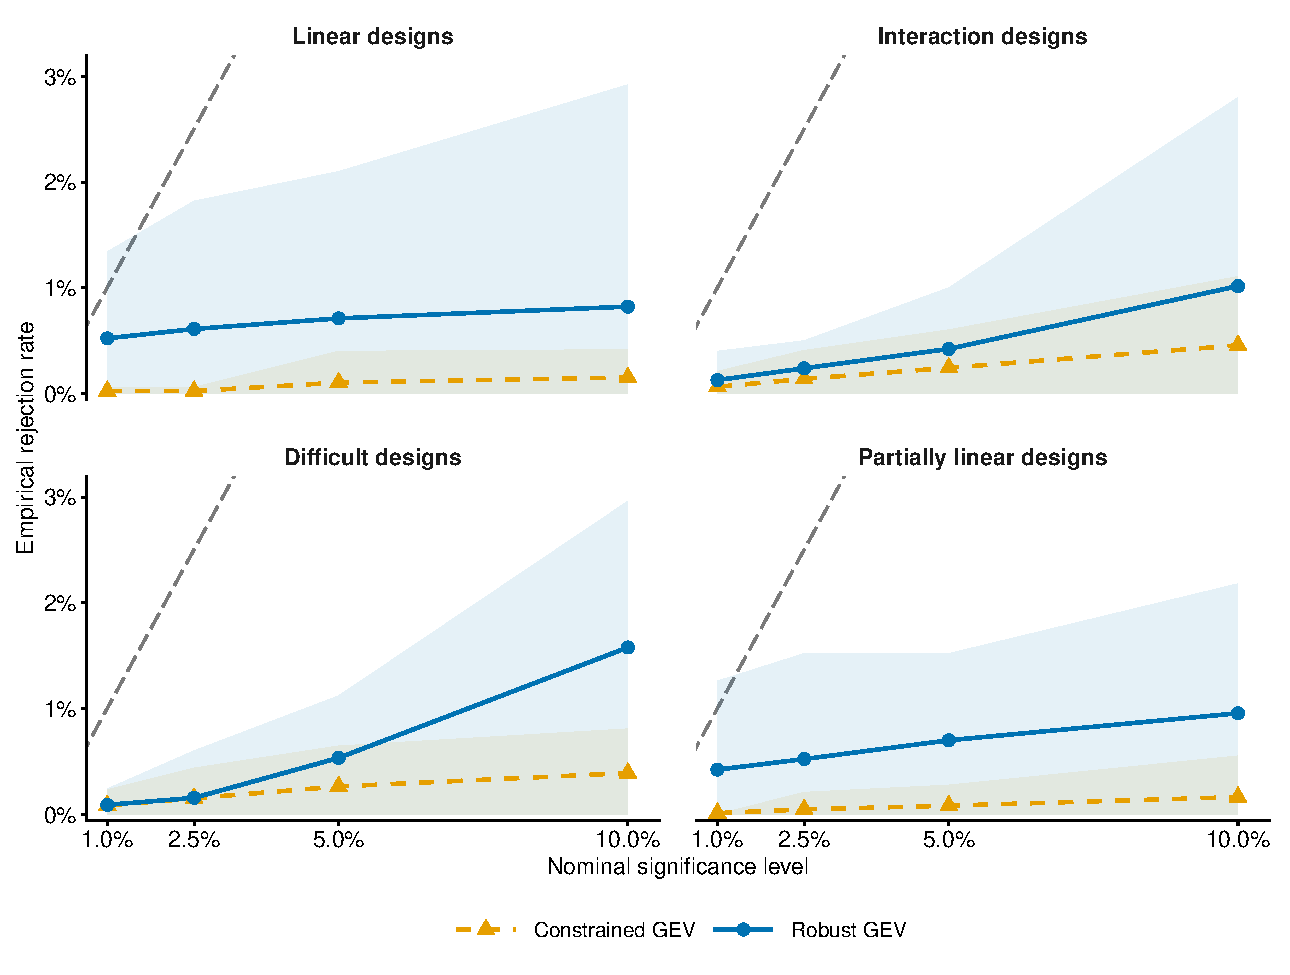
\includegraphics[width=\textwidth]{../../output/03_algorithmic/figures/main/03_fig3_null_calibration.pdf}
	\caption{Empirical null rejection rates across nominal significance levels for constrained and robust GEV fitting. The diagonal reference denotes equality between nominal and empirical rejection.}
	\label{fig:03-null-calibration}
\end{figure}

\begin{table}[htbp]
\centering
\caption{Empirical null rejection rates and convergence by GEV fitting method. Rejection-rate brackets report the 10th and 90th percentiles across architecture, sample-size, and set-size cells.}
\label{tab:03-null-calibration}
\resizebox{\columnwidth}{!}{%
\begin{tabular}{@{}lrrrrr@{}}
\toprule
GEV fitting method & Nominal 1\% & Nominal 2.5\% & Nominal 5\% & Nominal 10\% & Convergence, mean [P10, P90] \\
\midrule
Constrained GEV & 0.0\% [0.0, 0.2] & 0.1\% [0.0, 0.2] & 0.2\% [0.0, 0.6] & 0.3\% [0.0, 0.9] & 93.9\% [81.0, 100.0] \\
Robust GEV & 0.3\% [0.0, 0.8] & 0.4\% [0.0, 1.0] & 0.6\% [0.0, 1.4] & 1.0\% [0.0, 2.8] & 100.0\% [100.0, 100.0] \\
\bottomrule
\end{tabular}%
}
\end{table}


The architecture-specific calibration results lead to the same conclusion (\autoref{fig:03A-calibration-deviation} and \autoref{tab:03A-calibration-by-architecture}). At the nominal \(5\%\) level, architecture-level rejection remains well below \(5\%\) under both fits. The uniformity diagnostic also rejects the Uniform\((0,1)\) reference throughout the reported architecture summaries. The robust fit should therefore be interpreted as improving numerical convergence, not as restoring nominal p-value calibration in this particular stress-test design.

\begin{figure}[htbp]
	\centering
	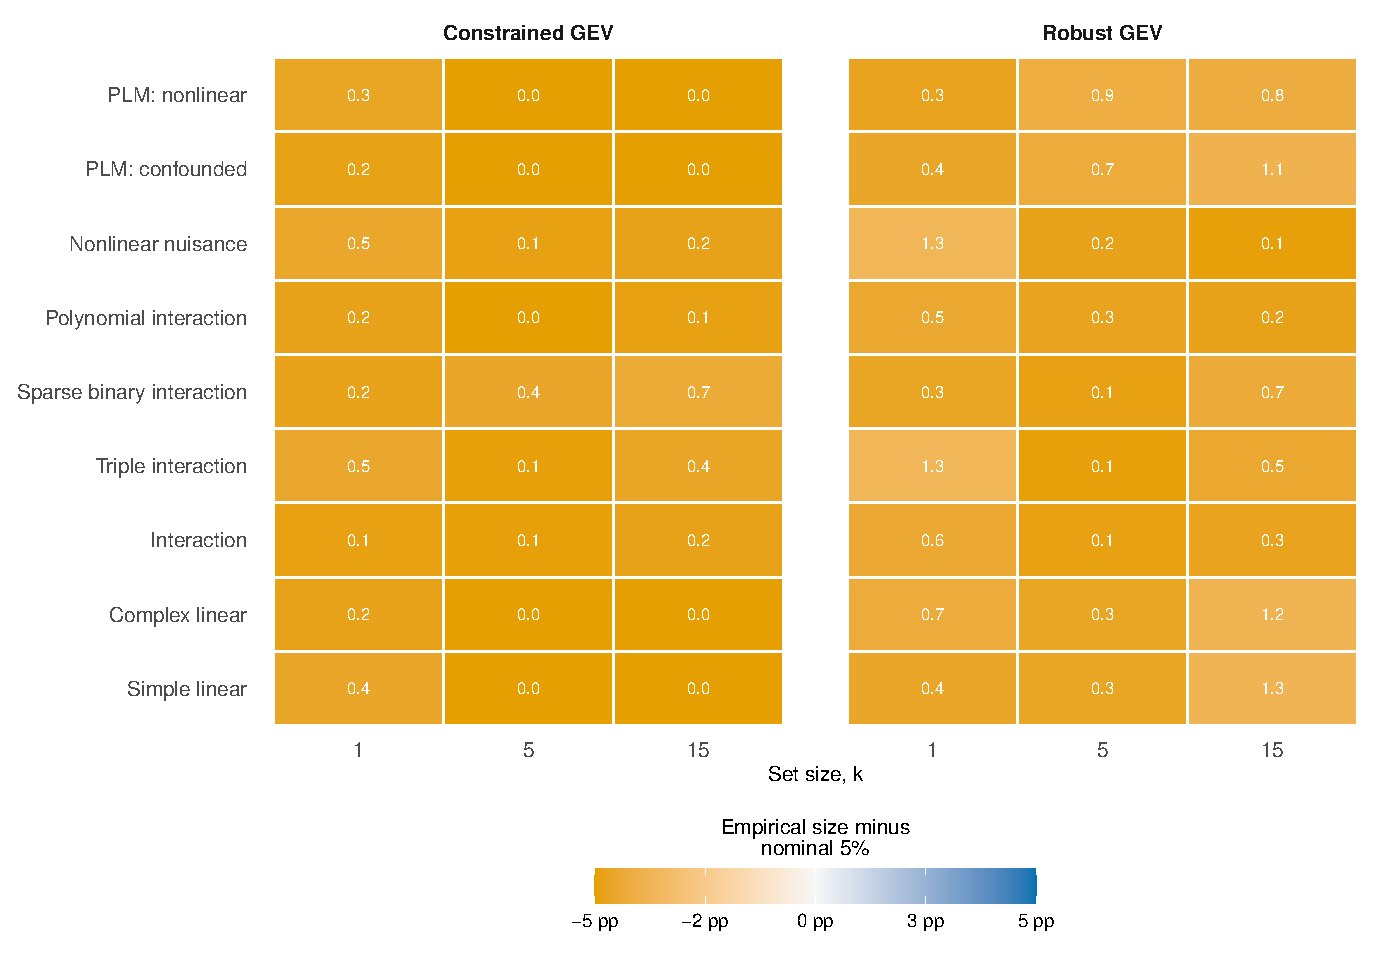
\includegraphics[width=\textwidth]{../../output/03_algorithmic/figures/supplement/03_figA3_calibration_deviation_heatmap.pdf}
	\caption{Architecture- and set-size-specific difference between empirical null rejection and the nominal \(5\%\) level for constrained and robust GEV fitting.}
	\label{fig:03A-calibration-deviation}
\end{figure}

\begin{table}[htbp]
\centering
\small
\caption{Null calibration, convergence, and fitted shape by architecture and GEV fitting method.}
\label{tab:03A-calibration-by-architecture}
\resizebox{\columnwidth}{!}{%
\begin{tabular}{@{}llrrrr@{}}
\toprule
Architecture & GEV fit & Size at 5\%, mean [P10, P90] & Convergence & KS p below 0.01 & Median shape \\
\midrule
Simple linear & Constrained GEV & 0.1\% [0.0, 0.4] & 93.2\% & 100.0\% & 0.000 \\
Simple linear & Robust GEV & 0.7\% [0.0, 1.4] & 100.0\% & 100.0\% & -0.000 \\
Complex linear & Constrained GEV & 0.1\% [0.0, 0.3] & 93.4\% & 100.0\% & 0.000 \\
Complex linear & Robust GEV & 0.8\% [0.0, 2.0] & 100.0\% & 100.0\% & -0.000 \\
Interaction & Constrained GEV & 0.1\% [0.0, 0.4] & 94.3\% & 100.0\% & 0.000 \\
Interaction & Robust GEV & 0.3\% [0.0, 0.8] & 100.0\% & 100.0\% & -0.000 \\
Triple interaction & Constrained GEV & 0.3\% [0.0, 0.6] & 92.5\% & 100.0\% & 0.000 \\
Triple interaction & Robust GEV & 0.6\% [0.0, 1.4] & 100.0\% & 100.0\% & 0.000 \\
Sparse binary interaction & Constrained GEV & 0.4\% [0.0, 1.3] & 96.3\% & 100.0\% & 0.000 \\
Sparse binary interaction & Robust GEV & 0.4\% [0.0, 0.8] & 100.0\% & 100.0\% & 0.296 \\
Polynomial interaction & Constrained GEV & 0.1\% [0.0, 0.4] & 93.8\% & 100.0\% & 0.000 \\
Polynomial interaction & Robust GEV & 0.3\% [0.0, 0.7] & 100.0\% & 100.0\% & -0.000 \\
Nonlinear nuisance & Constrained GEV & 0.3\% [0.0, 0.6] & 94.5\% & 100.0\% & -0.000 \\
Nonlinear nuisance & Robust GEV & 0.5\% [0.0, 1.1] & 100.0\% & 100.0\% & 0.000 \\
PLM: confounded & Constrained GEV & 0.1\% [0.0, 0.1] & 93.1\% & 100.0\% & 0.000 \\
PLM: confounded & Robust GEV & 0.8\% [0.0, 1.5] & 100.0\% & 100.0\% & -0.000 \\
PLM: nonlinear & Constrained GEV & 0.1\% [0.0, 0.3] & 94.1\% & 100.0\% & -0.000 \\
PLM: nonlinear & Robust GEV & 0.6\% [0.0, 1.3] & 100.0\% & 100.0\% & -0.000 \\
\bottomrule
\end{tabular}%
}
\end{table}


The null p-value quantile plots make the direction of the distortion explicit (\autoref{fig:03A-null-pvalue-qq}). Empirical p-values are substantially larger than the corresponding uniform theoretical quantiles, consistent with conservative rejection behaviour. This result qualifies the inferential evidence from the algorithmic validation study: the simulations support the computational use of Dinkelbach-based search and document strong numerical performance for robust GEV fitting, but they do not establish nominal EVT calibration across these architecture stress tests.

\begin{figure}[htbp]
	\centering
	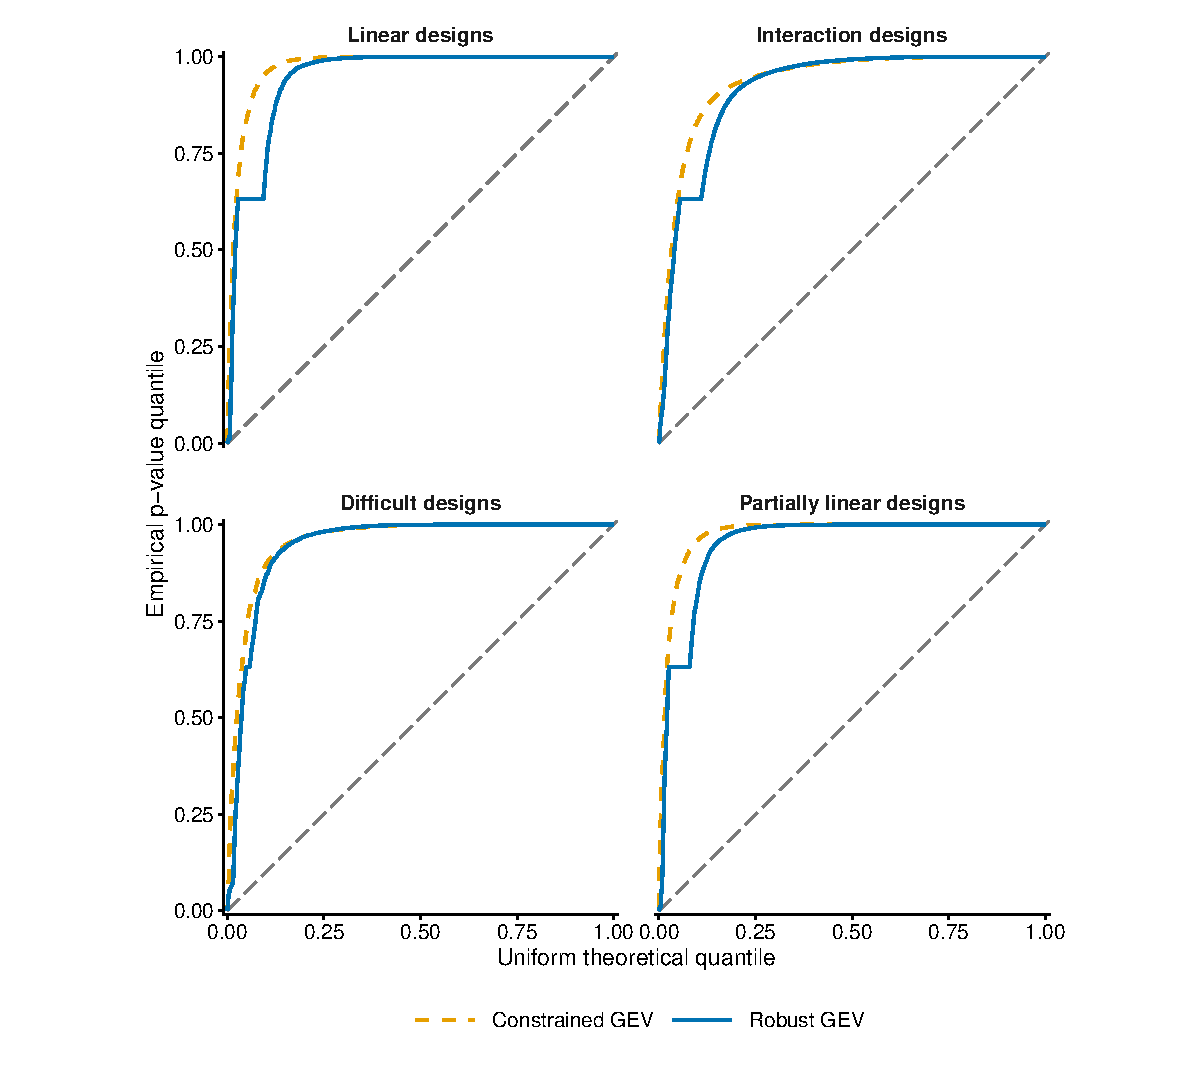
\includegraphics[width=\textwidth]{../../output/03_algorithmic/figures/supplement/03_figA5_null_pvalue_qq.pdf}
	\caption{Null p-value quantile plots for constrained and robust GEV fits across architecture groups. The diagonal denotes the Uniform\((0,1)\) reference.}
	\label{fig:03A-null-pvalue-qq}
\end{figure}

\subsection{Supplementary Robust-Estimation Results}
\label{app:estimation-results}

The formal robustness study contains \(1{,}248\) design cells and \(124{,}800\) Monte Carlo draws. Primary estimator summaries use the \(1{,}092\) finite-moment cells, while the GPD design is retained separately as an infinite-mean stress condition (\autoref{tab:robust-design-audit}).

\begin{table}[htbp]
\centering
\caption{Design audit for the formal Script 04 simulation. The primary analysis uses the seven finite-moment error distributions; GPD is retained separately as an infinite-mean stress condition.}
\label{tab:robust-design-audit}
\resizebox{0.7\columnwidth}{!}{%
\begin{tabular}{@{}lr@{}}
\toprule
Item & Value \\
\midrule
Total design cells & 1,248 \\
Iterations per cell & 100 \\
Total rows & 124,800 \\
Finite-moment primary cells & 1,092 \\
Finite-moment primary rows & 109,200 \\
GPD stress cells & 156 \\
GPD stress rows & 15,600 \\
Sample sizes & 500, 1000, 2500, 5000 \\
Contamination proportions & 0.5\%, 1\%, 2.5\%, 5\% \\
Predictor families & 3 \\
Error families & 8 \\
Contamination mechanisms & 3 + clean \\
\bottomrule
\end{tabular}%
}
\end{table}


MIS is evaluated as an oracle benchmark for both the injected-set size and the direction of the induced target-coefficient perturbation. Observation identities are not supplied to the search. The oracle audit confirms that \(k\) matches the injected-set size in every contaminated draw and shows that the mean absolute oracle coefficient shift is \(1.902\) under bad leverage, compared with \(0.020\) under response-outlier contamination and \(0.003\) under good leverage (\autoref{tab:robust-oracle-audit}).

\begin{table}[htbp]
\centering
\caption{Oracle benchmark audit. MIS is supplied the injected-set size and the oracle coefficient direction. Observation identities are then selected by the Dinkelbach-based search.}
\label{tab:robust-oracle-audit}
\resizebox{0.85\columnwidth}{!}{%
\begin{tabular}{@{}lrrrrr@{}}
\toprule
Scenario & Draws & Oracle k match & Positive direction & Negative direction & Mean absolute oracle shift \\
\midrule
Bad leverage & 33600 & 100.0\% & 50.0\% & 50.0\% & 1.902 \\
Good leverage & 33600 & 100.0\% & 49.8\% & 50.2\% & 0.003 \\
Response outliers & 33600 & 100.0\% & 50.4\% & 49.6\% & 0.020 \\
\bottomrule
\end{tabular}%
}
\end{table}


\subsubsection{Distributional and Data-Generating-Process Variation}
\label{app:estimation-dgp}

The full absolute-bias distributions provide additional detail on the aggregate results reported in Section~\ref{subsec:estimation-performance}. MM and LTS remain concentrated near zero across the principal finite-moment contamination mechanisms, while the diagnostic-removal estimators exhibit wider distributions in mechanism-specific settings (\autoref{fig:04A-absolute-bias}). MIS with oracle \(k\) shows wider absolute-error distributions under response-outlier and good-leverage contamination. Under bad leverage, its distribution contracts substantially relative to OLS, consistent with the much larger target-coefficient perturbation induced by the injected set.

\begin{figure}[htbp]
	\centering
	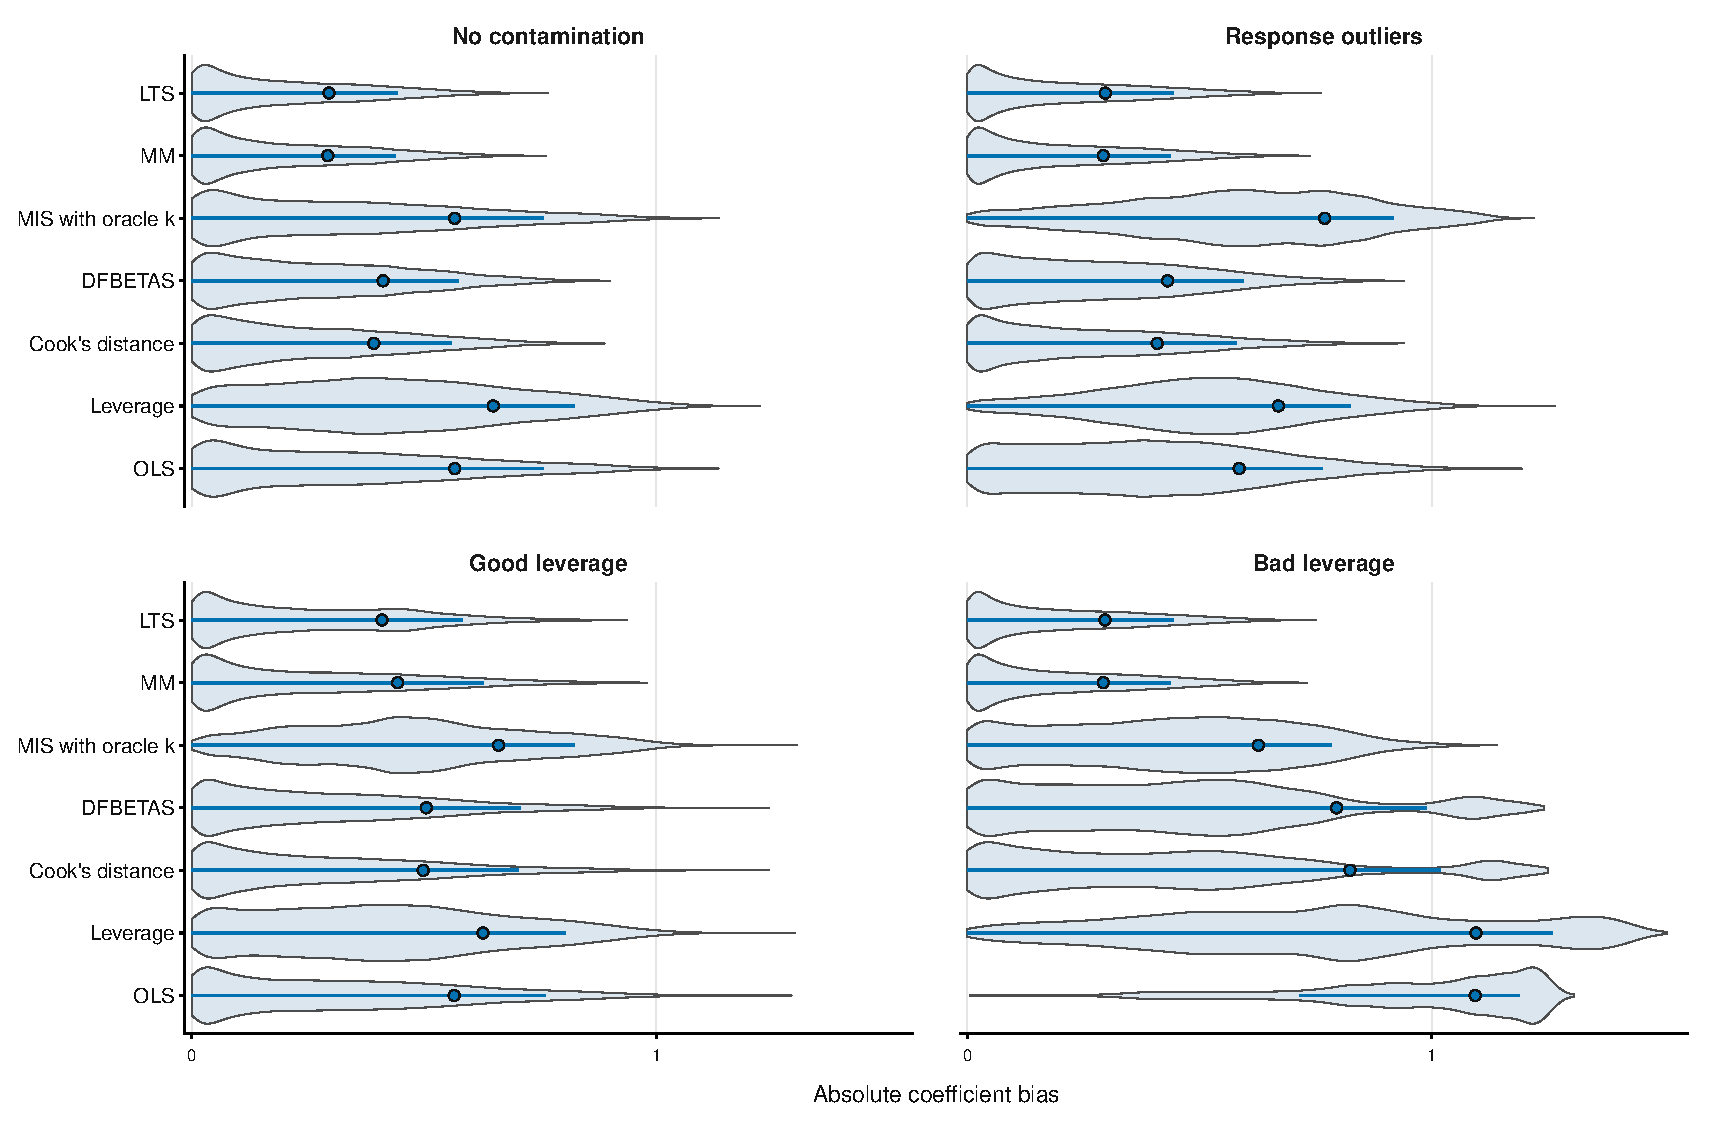
\includegraphics[width=\textwidth]{../../output/04_robust/figures/supplement/04_figA1_absolute_bias_distributions.pdf}
	\caption{Empirical distributions of absolute coefficient bias by estimator and contamination mechanism.}
	\label{fig:04A-absolute-bias}
\end{figure}

Error distributions generate substantial heterogeneity in coefficient accuracy (\autoref{fig:04A-bias-error}). The relative ordering of the diagnostic-removal estimators changes across error environments, while MM and LTS retain comparatively small mean absolute bias across most of the finite-moment designs. Predictor distributions also alter the magnitude of the post-deletion error (\autoref{fig:04A-bias-x}). These results show that pooled estimator summaries can conceal important interactions between the contamination mechanism and the surrounding data-generating environment.

\begin{figure}[htbp]
	\centering
	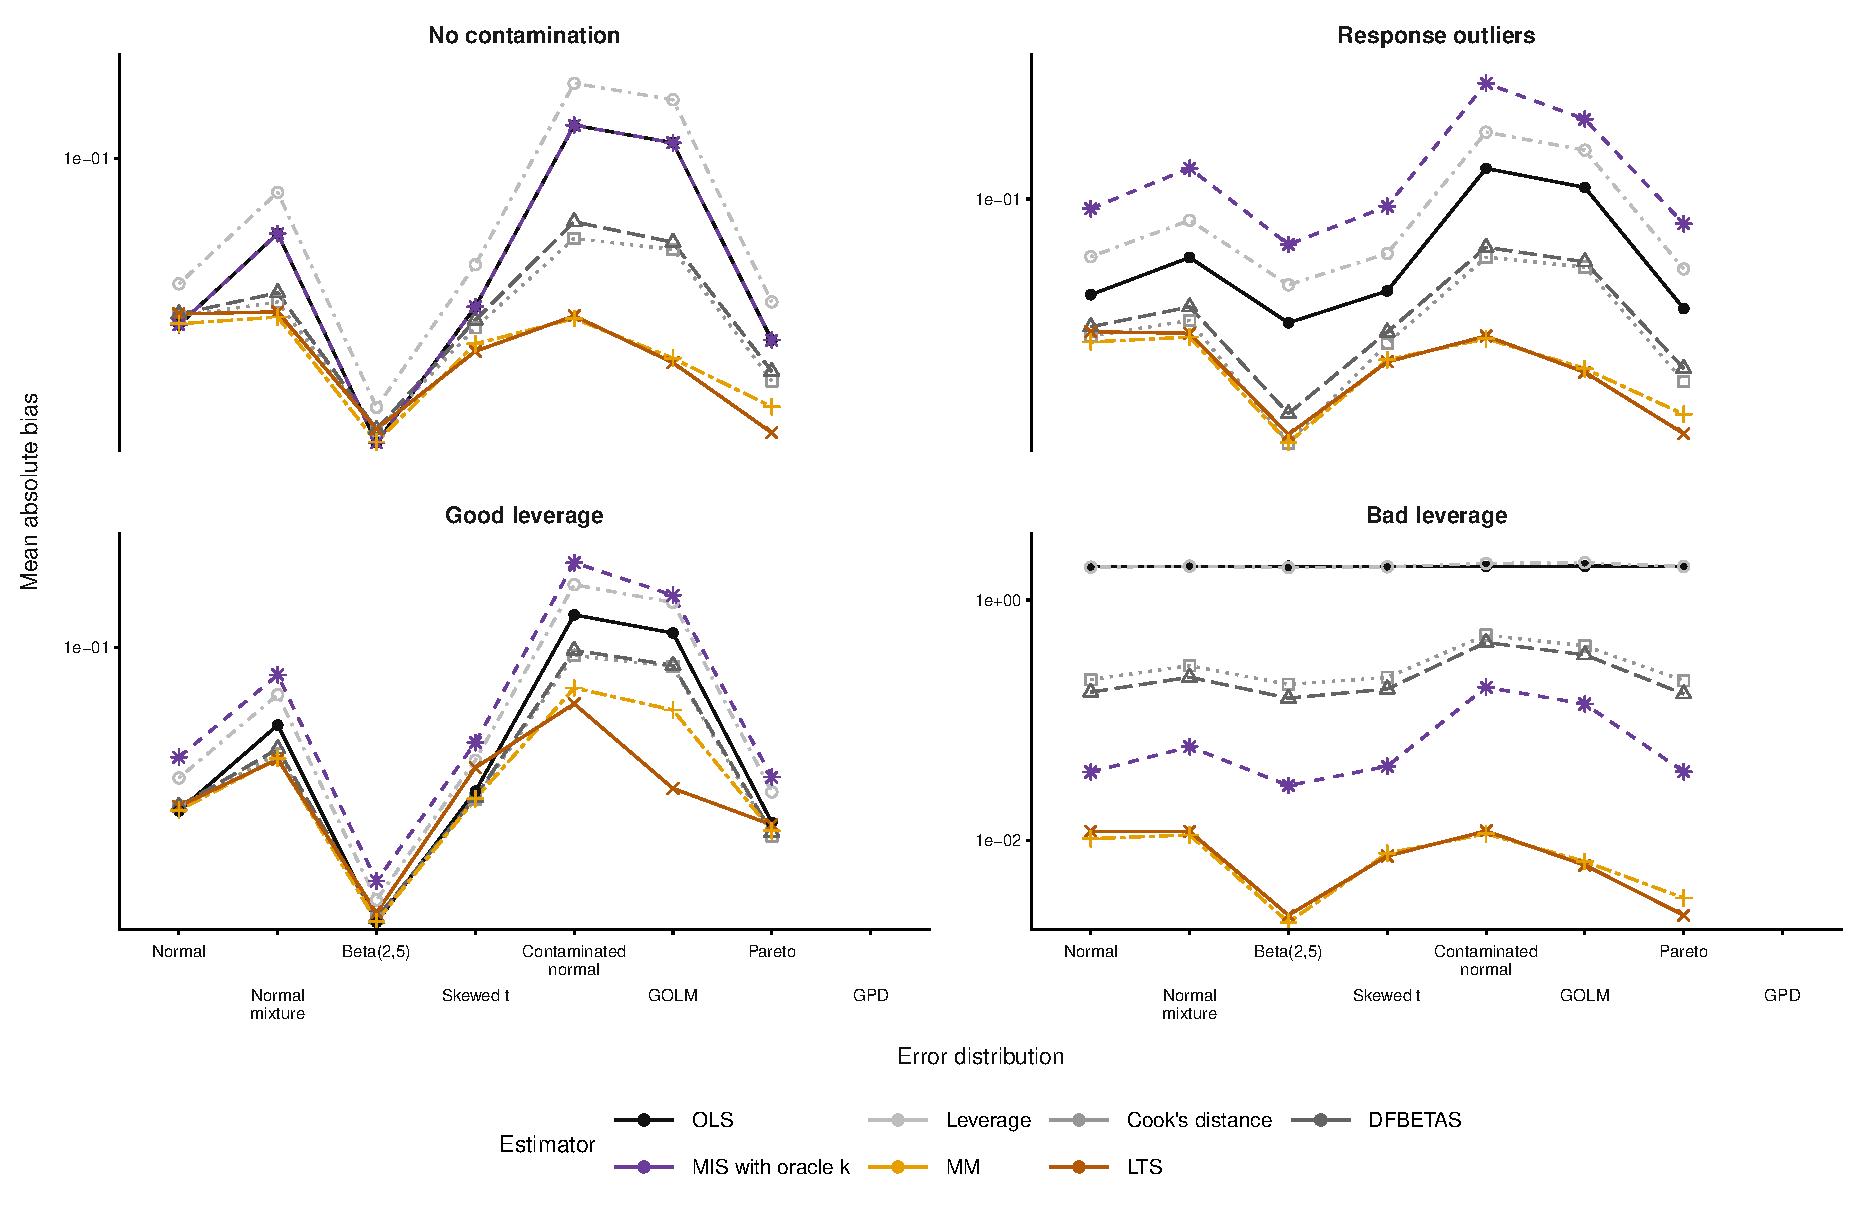
\includegraphics[width=\textwidth]{../../output/04_robust/figures/supplement/04_figA2_mean_bias_by_error_distribution.pdf}
	\caption{Mean absolute coefficient bias by estimator, error distribution, and contamination mechanism.}
	\label{fig:04A-bias-error}
\end{figure}

\begin{figure}[htbp]
	\centering
	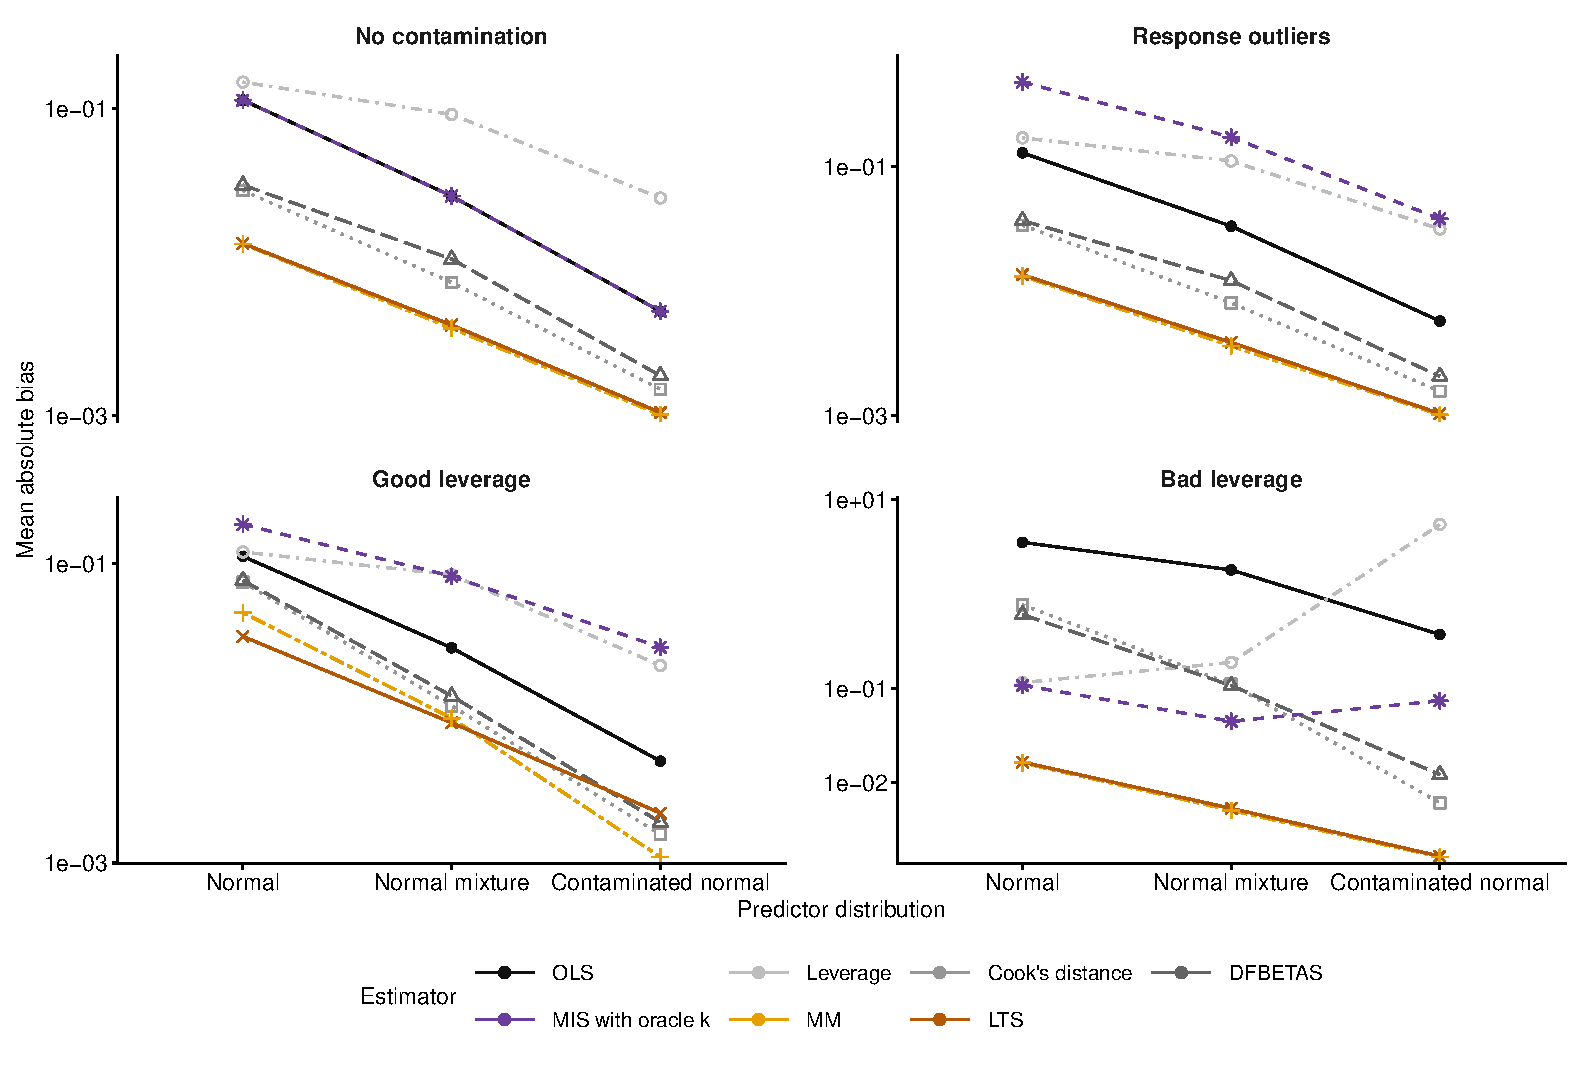
\includegraphics[width=\textwidth]{../../output/04_robust/figures/supplement/04_figA3_mean_bias_by_x_distribution.pdf}
	\caption{Mean absolute coefficient bias by estimator, predictor distribution, and contamination mechanism.}
	\label{fig:04A-bias-x}
\end{figure}

\subsubsection{Oracle-Benchmark MIS under Bad Leverage}
\label{app:oracle-k-detail}

The relative-error comparisons emphasise the mechanism specificity of the oracle-\(k\) benchmark. Relative to OLS, MIS with oracle \(k\) has lower mean absolute bias throughout the displayed bad-leverage finite-moment designs, often by a large margin (\autoref{fig:04A-mis-oracle-bias-advantage}). The corresponding differences are negative under vertical-outlier and good-leverage contamination. This pattern reflects the stronger alignment between bad leverage and the coefficient-targeted MIS objective.

\begin{figure}[htbp]
	\centering
	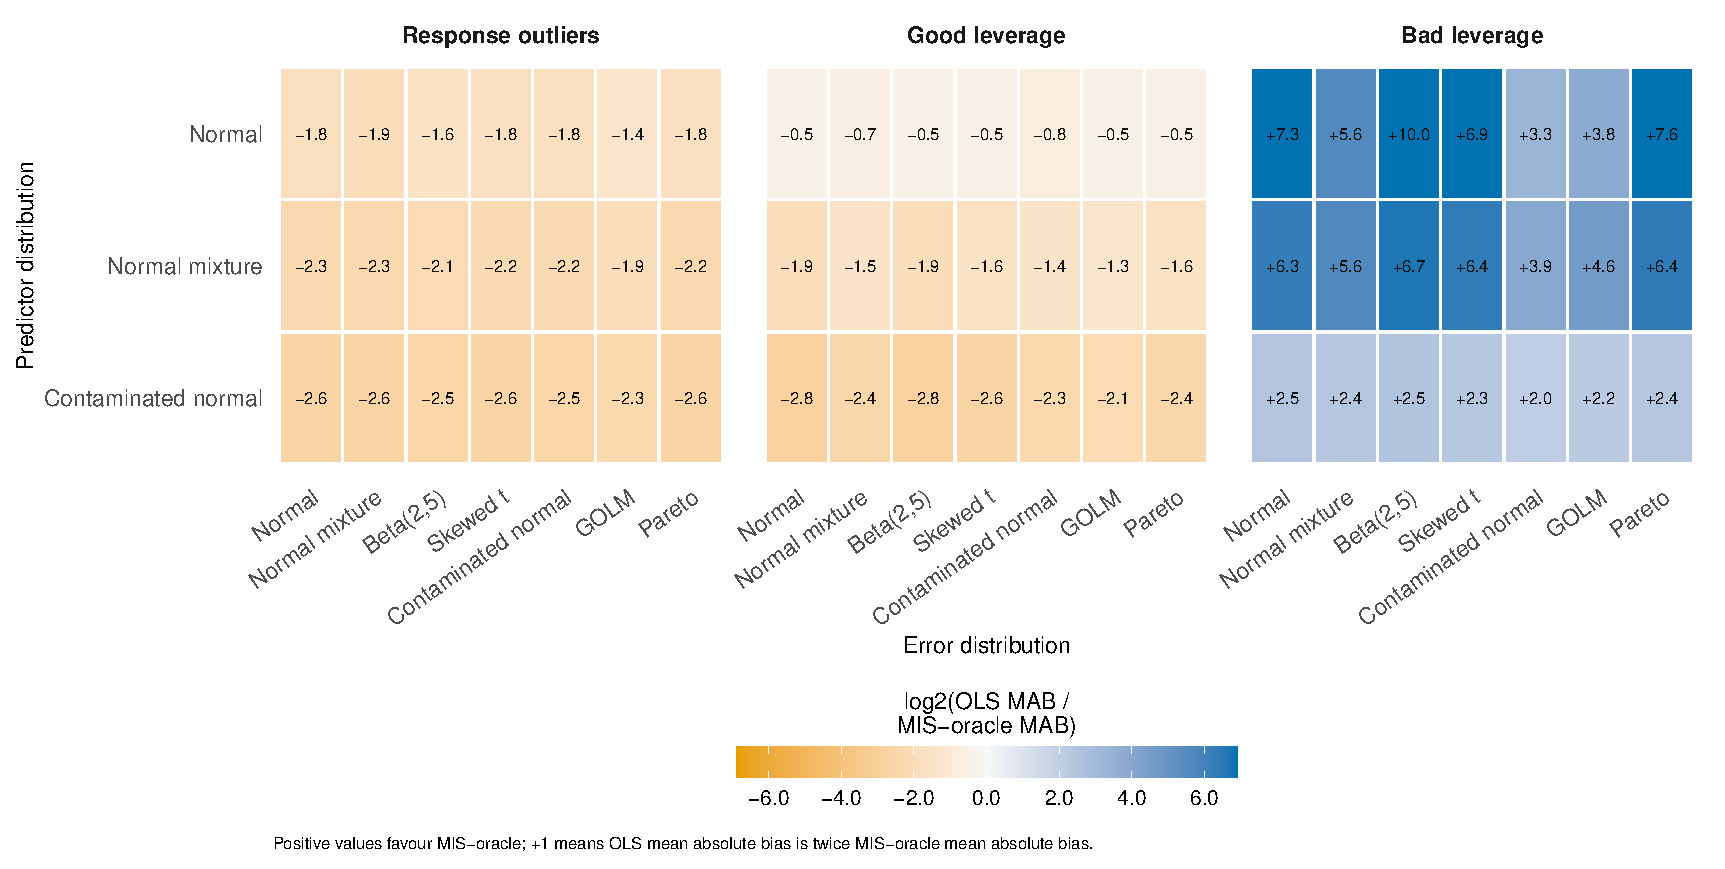
\includegraphics[width=\textwidth]{../../output/04_robust/figures/supplement/04_figA5_mis_oracle_bias_advantage_heatmap.pdf}
	\caption{Relative mean absolute bias of OLS and MIS with oracle \(k\) across predictor distributions, error distributions, and contamination mechanisms. Values report \(\log_2(\mathrm{MAB}_{\mathrm{OLS}}/\mathrm{MAB}_{\mathrm{MIS}})\); positive values indicate lower mean absolute bias for MIS with oracle \(k\).}
	\label{fig:04A-mis-oracle-bias-advantage}
\end{figure}

Comparison with the classical deletion procedures is more heterogeneous. Under bad leverage, MIS with oracle \(k\) compares favourably with leverage, Cook's distance, and DFBETAS in several normal and normal-mixture predictor environments, whereas the contaminated-normal predictor design changes the ordering substantially (\autoref{fig:04A-mis-oracle-vs-classical}). In that environment, extreme leverage can arise from the background predictor distribution as well as from the deliberately injected set. Deleting the injected observations therefore does not uniquely determine the geometry of the refitted sample. Cook's distance and DFBETAS can consequently produce a smaller post-deletion coefficient error despite recovering the injected set less selectively. This variation separates localisation accuracy from post-deletion estimation accuracy.

\begin{figure}[htbp]
	\centering
	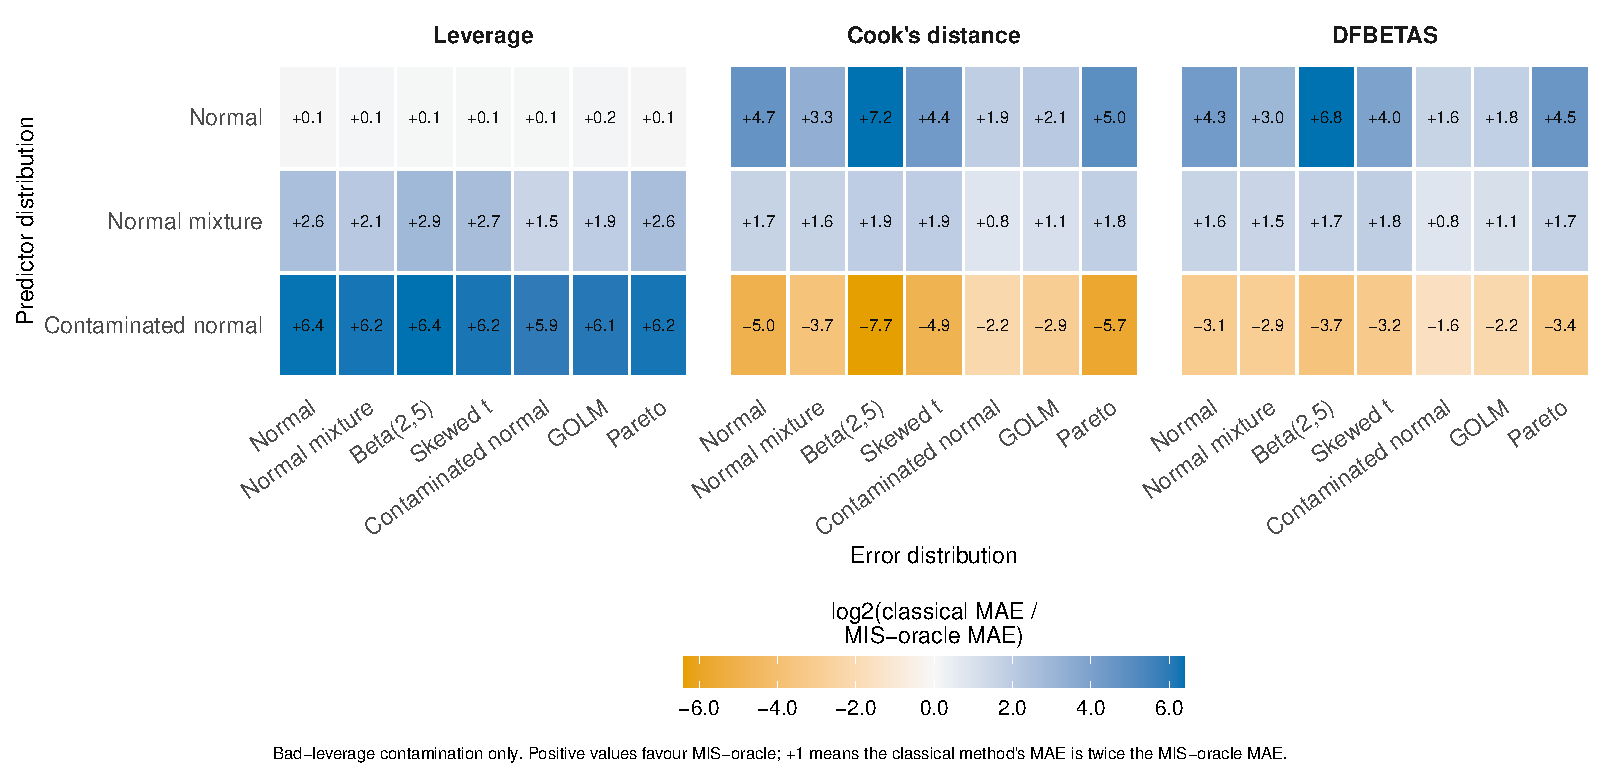
\includegraphics[width=\textwidth]{../../output/04_robust/figures/supplement/04_figA6_mis_oracle_vs_classical_bad_leverage_heatmap.pdf}
	\caption{Relative mean absolute error of leverage, Cook's distance, and DFBETAS deletion compared with MIS with oracle \(k\) under bad-leverage contamination. Values report \(\log_2(\mathrm{MAE}_{\mathrm{classical}}/\mathrm{MAE}_{\mathrm{MIS}})\); positive values indicate lower mean absolute error for MIS with oracle \(k\).}
	\label{fig:04A-mis-oracle-vs-classical}
\end{figure}

The predictor-level summary makes this reversal explicit (\autoref{tab:robust-bad-leverage-by-predictor}). With normal predictors, mean absolute bias is \(0.108\) for MIS, compared with \(0.771\) for Cook's distance and \(0.607\) for DFBETAS. Under the normal-mixture design, the corresponding values are \(0.045\), \(0.111\), and \(0.108\). Under contaminated-normal predictors, however, Cook's distance and DFBETAS fall to \(0.006\) and \(0.012\), while MIS records \(0.074\). The pooled bad-leverage comparison therefore does not imply uniform estimator ordering across predictor environments.

\begin{table}[htbp]
\centering
\caption{Bad-leverage mean absolute coefficient bias by predictor distribution. Results give equal weight to the recorded sample-size, contamination-proportion, and finite-moment error-distribution design cells.}
\label{tab:robust-bad-leverage-by-predictor}
\resizebox{0.7\columnwidth}{!}{%
\begin{tabular}{@{}llr@{}}
\toprule
Predictor & Estimator & Mean absolute bias \\
\midrule
Normal & OLS & 3.533 \\
Normal & Leverage & 0.116 \\
Normal & Cook's distance & 0.771 \\
Normal & DFBETAS & 0.607 \\
Normal & MIS with oracle k & 0.108 \\
Normal & MM & 0.016 \\
Normal & LTS & 0.017 \\
Normal mixture & OLS & 1.803 \\
Normal mixture & Leverage & 0.190 \\
Normal mixture & Cook's distance & 0.111 \\
Normal mixture & DFBETAS & 0.108 \\
Normal mixture & MIS with oracle k & 0.045 \\
Normal mixture & MM & 0.005 \\
Normal mixture & LTS & 0.005 \\
Contaminated normal & OLS & 0.374 \\
Contaminated normal & Leverage & 5.471 \\
Contaminated normal & Cook's distance & 0.006 \\
Contaminated normal & DFBETAS & 0.012 \\
Contaminated normal & MIS with oracle k & 0.074 \\
Contaminated normal & MM & 0.001 \\
Contaminated normal & LTS & 0.001 \\
\bottomrule
\end{tabular}%
}
\end{table}


\subsubsection{Runtime and Numerical Availability}
\label{app:estimation-computation}

The computational comparison shows that fixed-\(k\) MIS is slower than the classical diagnostic-removal procedures but substantially faster than the direct robust estimators in the revised implementation. Under contaminated designs, mean MIS runtime is approximately \(0.006\) seconds per draw, compared with roughly \(0.002\)--\(0.003\) seconds for the classical diagnostics, \(0.052\) seconds for LTS, and \(0.50\) seconds for MM (\autoref{tab:robust-runtime}). Under no contamination, MIS performs no deletion search because oracle \(k=0\). The complete runtime distributions are shown in \autoref{fig:04A-runtime}.

\begin{figure}[htbp]
	\centering
	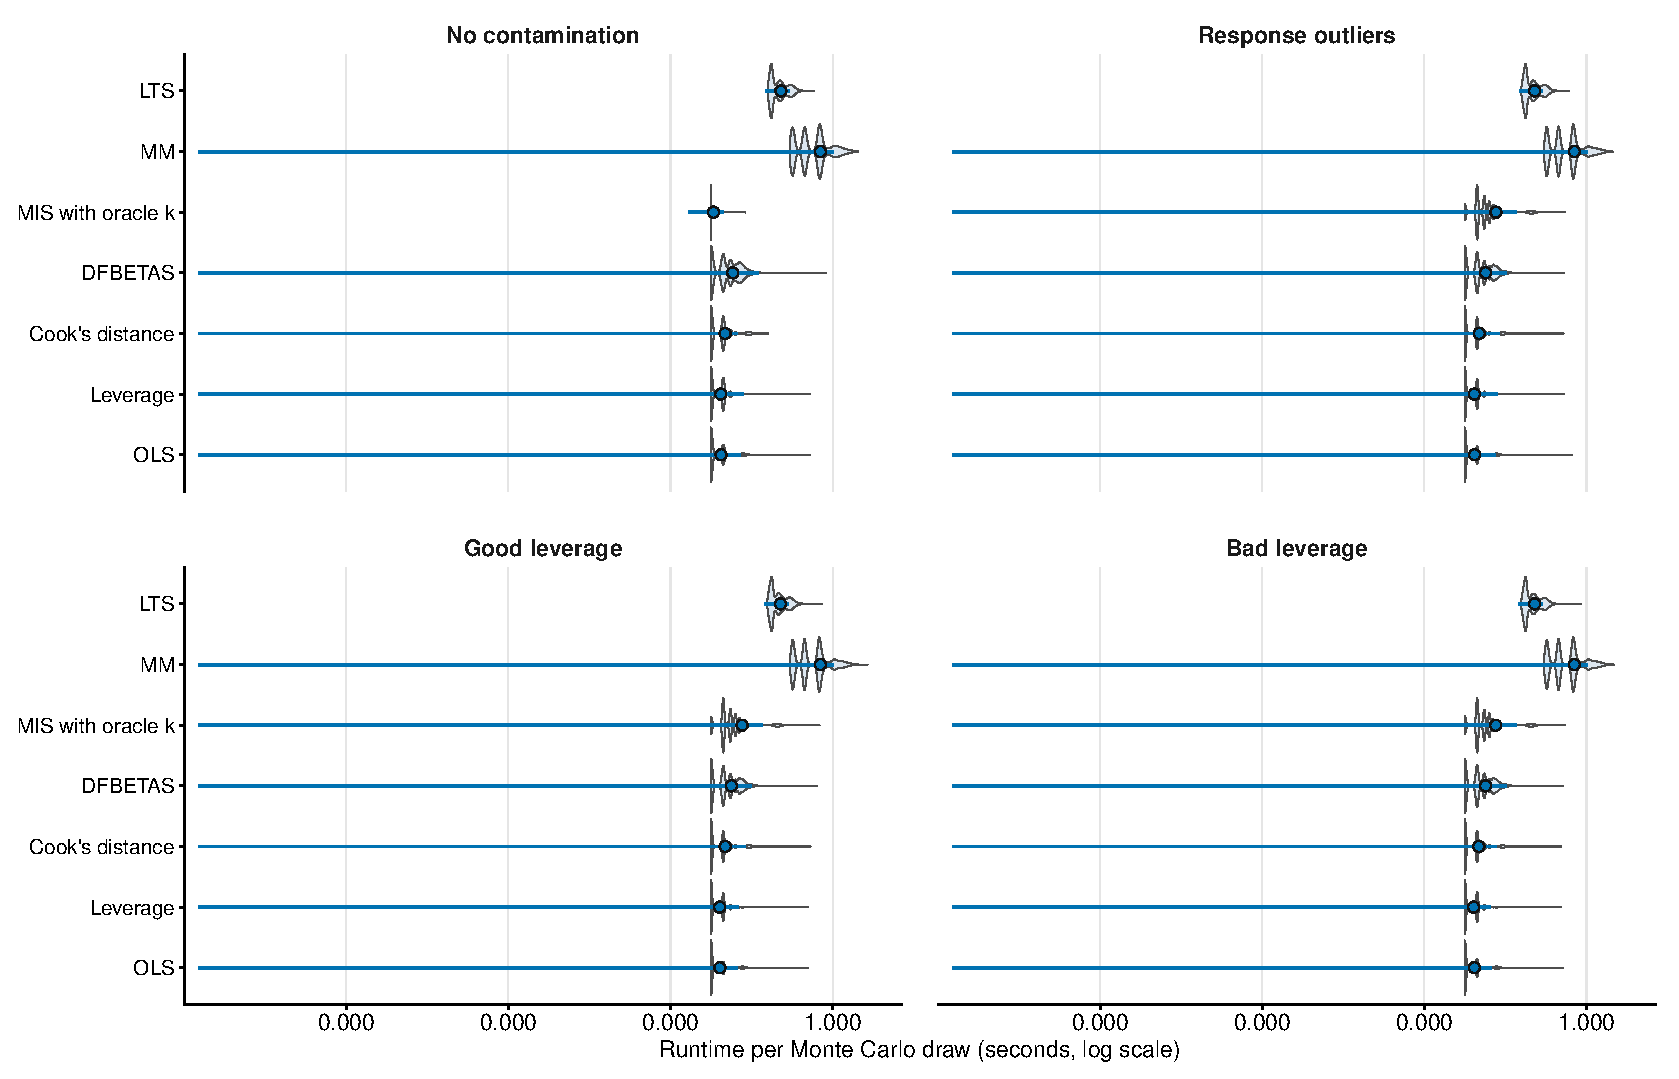
\includegraphics[width=\textwidth]{../../output/04_robust/figures/supplement/04_figA4_runtime_distributions.pdf}
	\caption{Empirical distributions of complete runtime per Monte Carlo draw by estimator and contamination mechanism. The horizontal axis uses a logarithmic scale.}
	\label{fig:04A-runtime}
\end{figure}

\begin{table}[htbp]
\centering
\caption{Mean complete runtime in seconds by estimator and contamination mechanism. Monte Carlo standard errors are in parentheses.}
\label{tab:robust-runtime}
\resizebox{0.85\columnwidth}{!}{%
\begin{tabular}{@{}lrrrr@{}}
\toprule
Estimator & None & Response outliers & Good leverage & Bad leverage \\
\midrule
OLS & 0.002 (0.000) & 0.002 (0.000) & 0.001 (0.000) & 0.002 (0.000) \\
Leverage & 0.002 (0.000) & 0.002 (0.000) & 0.002 (0.000) & 0.002 (0.000) \\
Cook's distance & 0.002 (0.000) & 0.002 (0.000) & 0.002 (0.000) & 0.002 (0.000) \\
DFBETAS & 0.003 (0.000) & 0.003 (0.000) & 0.003 (0.000) & 0.003 (0.000) \\
MIS with oracle k & 0.000 (0.000) & 0.006 (0.000) & 0.006 (0.000) & 0.006 (0.000) \\
MM & 0.499 (0.003) & 0.501 (0.002) & 0.499 (0.002) & 0.500 (0.002) \\
LTS & 0.053 (0.000) & 0.052 (0.000) & 0.052 (0.000) & 0.052 (0.000) \\
\bottomrule
\end{tabular}%
}
\end{table}


Numerical availability was complete for every estimator in the primary finite-moment analysis. All \(109{,}200\) recorded rows for each method produced finite coefficient estimates, coverage indicators, and runtimes (\autoref{tab:robust-method-health}). The reported differences therefore reflect statistical performance across the simulation grid rather than differential numerical non-completion.

\begin{table}[htbp]
\centering
\caption{Method-level availability and numerical health checks.}
\label{tab:robust-method-health}
\resizebox{0.7\columnwidth}{!}{%
\begin{tabular}{@{}lrrrr@{}}
\toprule
Estimator & Total rows & Finite coefficient & Finite coverage & Finite runtime \\
\midrule
OLS & 109200 & 100.0\% & 100.0\% & 100.0\% \\
Leverage & 109200 & 100.0\% & 100.0\% & 100.0\% \\
Cook's distance & 109200 & 100.0\% & 100.0\% & 100.0\% \\
DFBETAS & 109200 & 100.0\% & 100.0\% & 100.0\% \\
MIS with oracle k & 109200 & 100.0\% & 100.0\% & 100.0\% \\
MM & 109200 & 100.0\% & 100.0\% & 100.0\% \\
LTS & 109200 & 100.0\% & 100.0\% & 100.0\% \\
\bottomrule
\end{tabular}%
}
\end{table}









\subsection{Supplementary Misspecification Results}
\label{app:misspecification-results}

\subsubsection{Misspecification Severity and Operating-Characteristic Definitions}
\label{app:misspec-definitions}

The detector experiment uses the baseline model
\[
Y_i=\beta_0+\beta_1X_i+m_i+\varepsilon_i,
\qquad
\beta_0=0,
\qquad
\beta_1=1.
\]
For the additive misspecification mechanisms, a raw component \(h_i\) is scaled according to
\[
a_\lambda
=
\lambda
\frac{\operatorname{sd}(\varepsilon_0)}
{\operatorname{sd}(h)},
\qquad
m_i=a_\lambda h_i,
\]
so that
\[
\frac{\operatorname{sd}(m)}
{\operatorname{sd}(\varepsilon_0)}
=
\lambda.
\]
Thus \(\lambda\) has a common signal-to-noise interpretation for nonlinearity, threshold behaviour, omitted-variable misspecification, heterogeneous slopes, and missing interactions. Equality of this signal-to-noise ratio makes the additive severity scale comparable in construction, although the substantive form of the imposed departure still differs across mechanisms. Heteroskedasticity instead uses an exponential spread-gradient parameter, while linear endogeneity and nonlinear confounding use mechanism-specific confounding-strength parameters. Detection boundaries are therefore interpreted within the corresponding severity scale.

The MIS comparison index is
\[
T_k
=
\frac{
	\left|
	\widehat{\beta}_{-S_k}-\widehat{\beta}
	\right|
}{
	\widehat{\operatorname{se}}(\widehat{\beta})
}.
\]
The denominator is the standard error from the original fitted model and is held fixed as the reference scale. Although \(T_k\) is measured in standard-error units, it is not treated as a Wald statistic. The full-sample and post-deletion estimates are dependent, the deletion set is selected adaptively, and the reported statistic is extremal over candidate deletions. A standard-normal reference distribution is therefore neither assumed nor used.

For an independently calibrated rejection indicator \(R_b(\lambda)\) in Monte Carlo draw \(b\), empirical power is
\[
\widehat{\pi}(\lambda)
=
\frac{1}{B}
\sum_{b=1}^{B}R_b(\lambda),
\]
and empirical size is \(\widehat{\pi}(0)\). The 80\% detection reach is the proportion of environments whose isotonic fitted power curve reaches \(0.80\) within the simulated severity range. For environments that cross this level, the detection boundary is the interpolated severity at which fitted power first reaches \(0.80\). Non-crossing environments are right-censored and are retained in the reach calculation.

For paired diagnostic comparisons, the MIS-only rejection probability is
\[
P(R_{\mathrm{MIS}}=1,R_{\mathrm{rival}}=0),
\]
and the rival-only probability is
\[
P(R_{\mathrm{MIS}}=0,R_{\mathrm{rival}}=1).
\]
These discordant-rejection probabilities are reported separately because they measure complementarity between diagnostics. Their difference may be summarised descriptively as a paired rejection difference, but the two component probabilities carry the substantive interpretation.

\subsubsection{Null Calibration and Scaling}
\label{app:misspec-calibration}

The standard-error normalisation does not make \(T_k\) pivotal. Its null distribution changes systematically with sample size and fitted model class, which is why calibration is performed within the relevant null environment. In particular, the null mean of the standardised statistic increases approximately with \(\sqrt{n}\), and correctly specified models containing additional regressors require their own null cutoffs. The calibration analysis therefore evaluates empirical size and cutoff stability directly rather than relying on Gaussian critical values. The detailed null results support the calibration used for the power comparisons in Section~\ref{subsec:misspecification}. Across error distributions, MIS empirical size at \(k/n=0.025\) remains close to \(5\%\), ranging from \(4.75\%\) to \(5.33\%\) (\autoref{tab:05-size-by-error}). The same stability appears across predictor distributions and sample sizes, where empirical rejection ranges from \(4.79\%\) to \(5.28\%\) (\autoref{tab:05-size-by-x-n}). The distribution of environment-level null rejection rates is shown in \autoref{fig:05S-size-calibration}.

\begin{figure}[htbp]
	\centering
	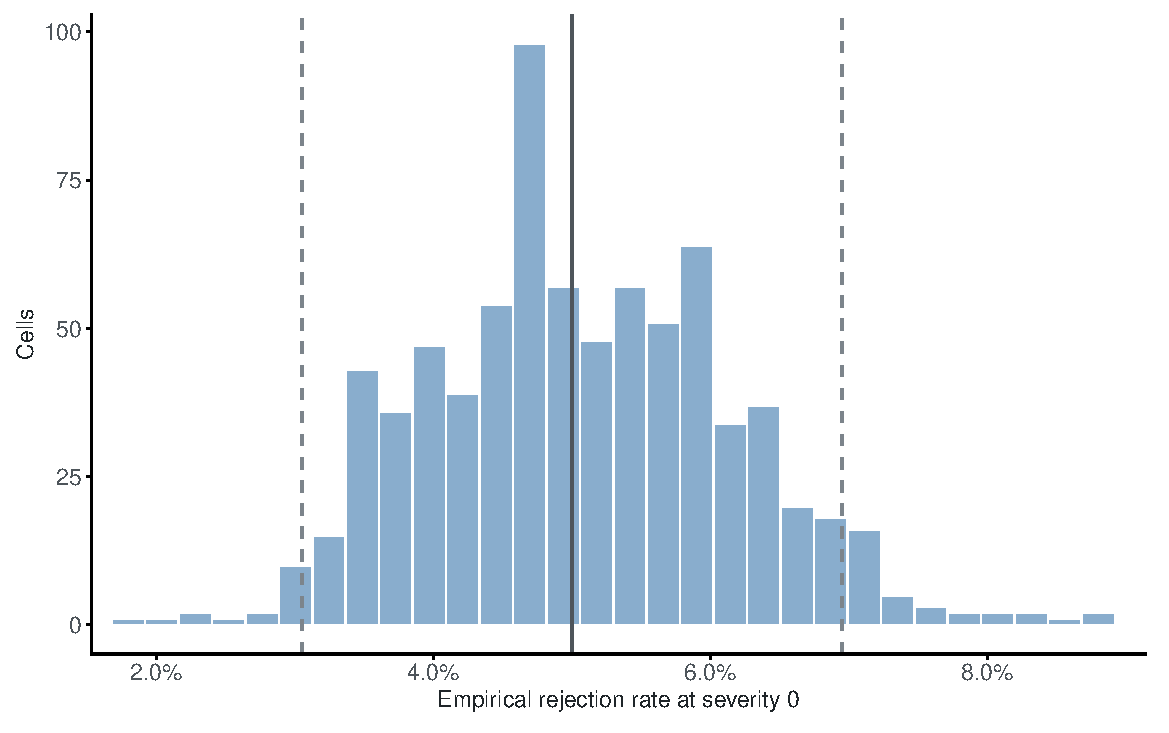
\includegraphics[width=0.82\textwidth]{../../output/05_misspecification/figures/supplement/05_figS01_empirical_size_histogram.pdf}
	\caption{Distribution of environment-level empirical MIS rejection rates at zero misspecification severity.}
	\label{fig:05S-size-calibration}
\end{figure}

\begin{table}[htbp]
\centering
\caption{Empirical size by error distribution at k/n = 2.5 percent for MIS, RESET, and BP.}
\label{tab:05-size-by-error}
\resizebox{0.85\columnwidth}{!}{%
\begin{tabular}{@{}lrrrrr@{}}
\toprule
Error distribution & MIS & RESET (cal.) & RESET (nom.) & BP (cal.) & BP (nom.) \\
\midrule
Beta-logistic & 4.93\% & 4.99\% & 7.24\% & 5.19\% & 4.73\% \\
Contaminated & 5.13\% & 4.98\% & 1.60\% & 4.97\% & 5.62\% \\
GOLM & 5.33\% & 5.07\% & 12.76\% & 5.14\% & 6.14\% \\
GPD & 5.00\% & 5.13\% & 8.78\% & 4.79\% & 5.79\% \\
Mixed normal & 5.25\% & 5.10\% & 2.57\% & 5.07\% & 5.59\% \\
Normal & 4.99\% & 4.76\% & 6.65\% & 5.03\% & 4.69\% \\
Pareto & 5.13\% & 4.84\% & 9.25\% & 5.11\% & 5.90\% \\
Skewed t & 4.75\% & 4.88\% & 7.14\% & 4.98\% & 5.78\% \\
\bottomrule
\end{tabular}%
}
\end{table}


\begin{table}[htbp]
\centering
\caption{MIS empirical size by X distribution and sample size at k/n = 2.5 percent.}
\label{tab:05-size-by-x-n}
\resizebox{0.70\columnwidth}{!}{%
\begin{tabular}{@{}lrr@{}}
\toprule
X distribution & n & MIS size \\
\midrule
Normal X & 500 & 5.15\% \\
Normal X & 1000 & 4.98\% \\
Normal X & 2500 & 5.17\% \\
Normal X & 5000 & 4.92\% \\
\addlinespace
Mixed-normal X & 500 & 5.21\% \\
Mixed-normal X & 1000 & 4.89\% \\
Mixed-normal X & 2500 & 5.02\% \\
Mixed-normal X & 5000 & 4.96\% \\
\addlinespace
Contaminated X & 500 & 5.22\% \\
Contaminated X & 1000 & 5.17\% \\
Contaminated X & 2500 & 5.28\% \\
Contaminated X & 5000 & 4.79\% \\
\bottomrule
\end{tabular}%
}
\end{table}


The magnitude of the null MIS statistic increases systematically with sample size even though its calibrated rejection probability remains stable. The fitted log--log slopes are \(0.470\), \(0.469\), and \(0.472\) for normal, mixed-normal, and contaminated predictor distributions, respectively, with \(R^2\) values above \(0.999\) (\autoref{fig:05S-null-scaling} and \autoref{tab:05-null-scaling}). This scaling result motivates environment-specific calibration rather than comparison of uncalibrated statistic magnitudes across sample sizes.

\begin{figure}[htbp]
	\centering
	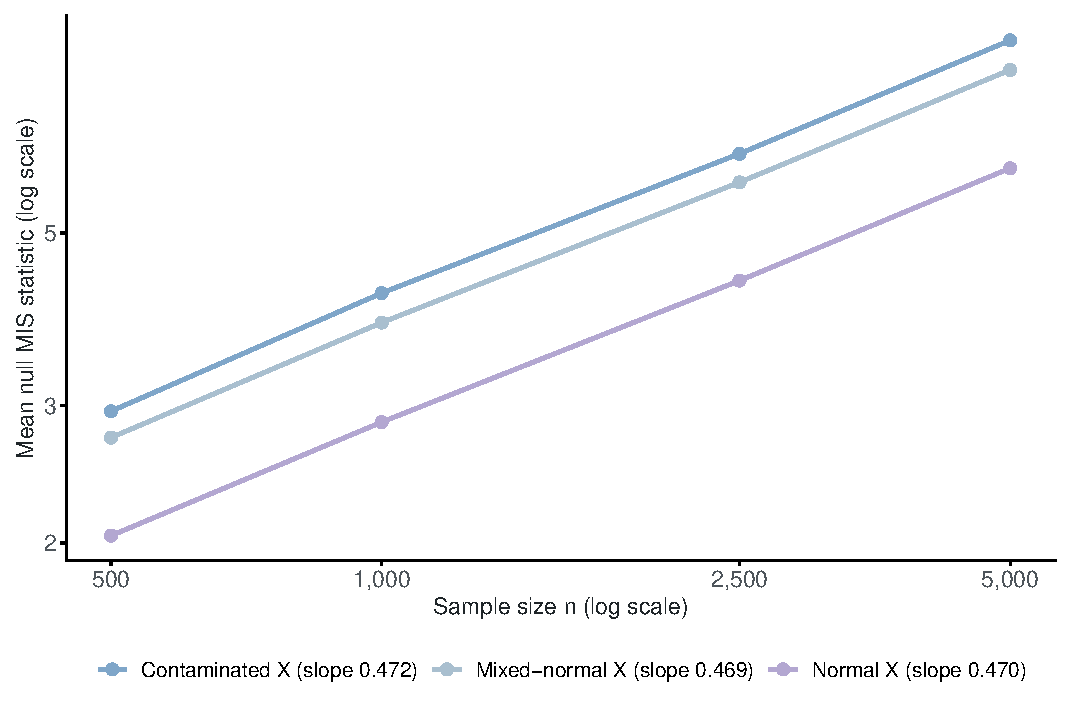
\includegraphics[width=0.82\textwidth]{../../output/05_misspecification/figures/supplement/05_figS02_null_scaling.pdf}
	\caption{Mean null MIS statistic by sample size and predictor distribution on logarithmic axes.}
	\label{fig:05S-null-scaling}
\end{figure}

\begin{table}[htbp]
\centering
\caption{Log-log scaling of the null mean MIS statistic with sample size.}
\label{tab:05-null-scaling}
\resizebox{0.70\columnwidth}{!}{%
\begin{tabular}{@{}lrr@{}}
\toprule
X distribution & Log-log slope & R-squared \\
\midrule
Normal X & 0.470 & 0.9999 \\
Mixed-normal X & 0.469 & 0.9998 \\
Contaminated X & 0.472 & 0.9996 \\
\bottomrule
\end{tabular}%
}
\end{table}


\subsubsection{Detailed Power and Environmental Heterogeneity}
\label{app:misspec-power}

The complete severity curves show that diagnostic sensitivity differs both across mechanisms and across methods (\autoref{fig:05S-power-severity}). MIS power rises rapidly for nonlinear confounding, heterogeneous slopes, missing interactions, nonlinearity, and threshold behaviour, while linear endogeneity remains close to its null rejection rate throughout the simulated range. The omitted-variable mechanism produces only a modest increase in pooled MIS power. RESET and Breusch--Pagan exhibit their own mechanism-specific profiles, reinforcing the distinction between general coefficient sensitivity and specialist specification tests.

\begin{figure}[htbp]
	\centering
	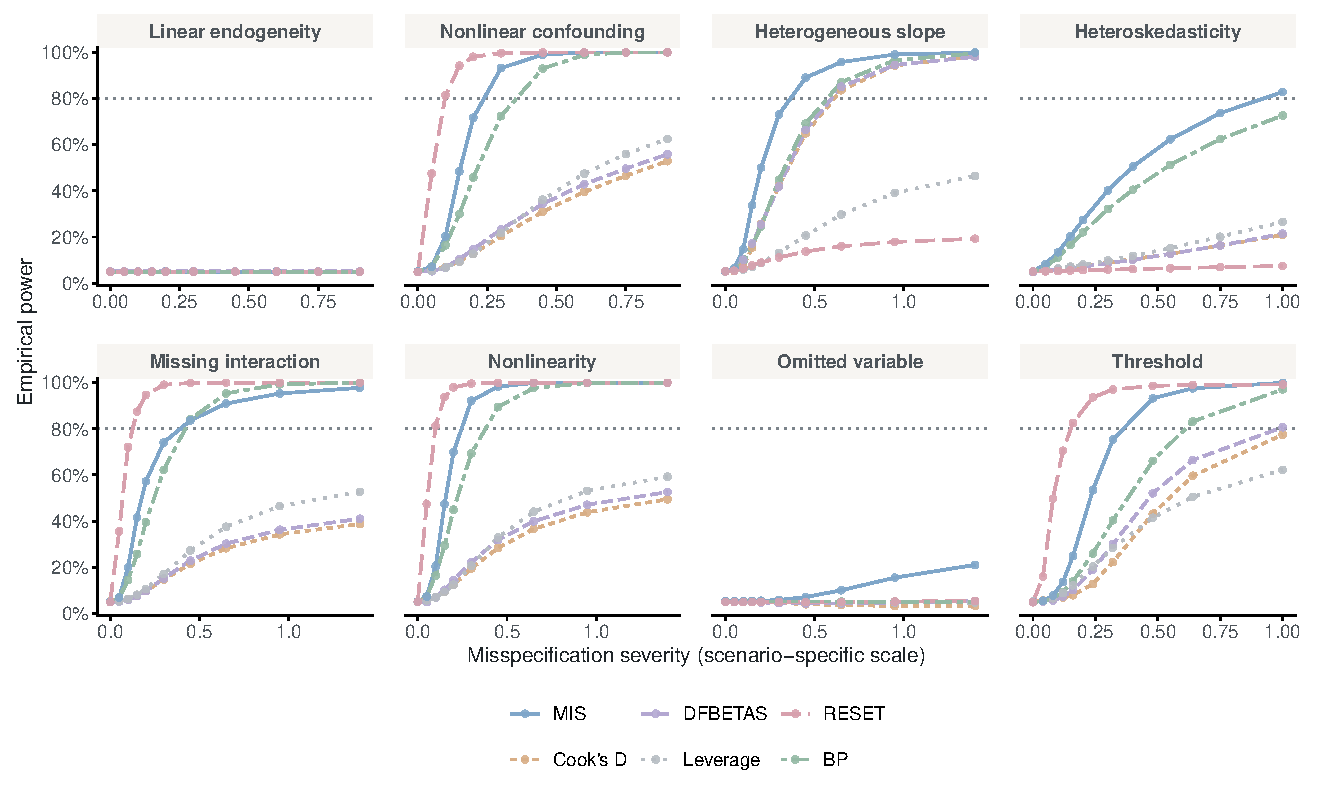
\includegraphics[width=\textwidth]{../../output/05_misspecification/figures/supplement/05_figS03_power_severity.pdf}
	\caption{Empirical power by misspecification severity for MIS, classical influence diagnostics, RESET, and Breusch--Pagan. Severity is defined on a scenario-specific scale.}
	\label{fig:05S-power-severity}
\end{figure}

Average power also varies across the surrounding error and predictor environments. MIS mean positive-severity power ranges from \(43.4\%\) under GOLM errors to \(51.9\%\) under normal errors, and from \(38.9\%\) with normal predictors to approximately \(51\%\) with mixed-normal and contaminated predictors (\autoref{tab:05-power-by-error} and \autoref{tab:05-power-by-x}). Average power increases with sample size from \(37.8\%\) at \(n=500\) to \(55.8\%\) at \(n=5000\) (\autoref{tab:05-power-by-n}).

\begin{table}[htbp]
\centering
\caption{Mean detection power across positive-severity simulation cells by error distribution at k/n = 2.5 percent; scenario-specific severity grids are retained.}
\label{tab:05-power-by-error}
\resizebox{\columnwidth}{!}{%
\begin{tabular}{@{}lrrrrrr@{}}
\toprule
Error distribution & MIS & Cook's D & DFBETAS & Leverage & RESET & BP \\
\midrule
Beta-logistic & 51.7\% & 20.9\% & 20.5\% & 19.3\% & 45.4\% & 54.1\% \\
Contaminated & 45.5\% & 16.2\% & 17.3\% & 18.4\% & 51.2\% & 37.4\% \\
GOLM & 43.4\% & 17.2\% & 21.7\% & 16.8\% & 47.4\% & 25.3\% \\
GPD & 44.9\% & 23.1\% & 22.7\% & 18.5\% & 45.5\% & 34.4\% \\
Mixed normal & 46.5\% & 18.0\% & 23.0\% & 18.6\% & 50.1\% & 38.5\% \\
Normal & 51.9\% & 22.3\% & 21.7\% & 18.9\% & 45.8\% & 53.6\% \\
Pareto & 44.1\% & 22.0\% & 23.5\% & 18.1\% & 45.5\% & 31.5\% \\
Skewed t & 47.4\% & 22.7\% & 21.8\% & 18.6\% & 45.3\% & 42.3\% \\
\bottomrule
\end{tabular}%
}
\end{table}


\begin{table}[htbp]
\centering
\caption{Mean detection power across positive-severity simulation cells by X distribution at k/n = 2.5 percent; scenario-specific severity grids are retained.}
\label{tab:05-power-by-x}
\resizebox{\columnwidth}{!}{%
\begin{tabular}{@{}lrrrrrr@{}}
\toprule
X distribution & MIS & Cook's D & DFBETAS & Leverage & RESET & BP \\
\midrule
Normal X & 38.9\% & 14.1\% & 14.9\% & 18.1\% & 47.0\% & 34.1\% \\
Mixed-normal X & 51.4\% & 23.8\% & 24.9\% & 19.4\% & 47.2\% & 42.3\% \\
Contaminated X & 50.5\% & 23.0\% & 24.7\% & 17.7\% & 46.9\% & 42.5\% \\
\bottomrule
\end{tabular}%
}
\end{table}


\begin{table}[htbp]
\centering
\caption{Mean detection power across positive-severity simulation cells by sample size at k/n = 2.5 percent; scenario-specific severity grids are retained.}
\label{tab:05-power-by-n}
\resizebox{0.85\columnwidth}{!}{%
\begin{tabular}{@{}lrrrrrr@{}}
\toprule
n & MIS & Cook's D & DFBETAS & Leverage & RESET & BP \\
\midrule
500 & 37.8\% & 17.6\% & 18.1\% & 17.4\% & 41.2\% & 33.6\% \\
1000 & 43.2\% & 19.2\% & 20.2\% & 17.7\% & 45.9\% & 37.2\% \\
2500 & 50.9\% & 21.6\% & 23.1\% & 18.8\% & 49.5\% & 42.1\% \\
5000 & 55.8\% & 22.9\% & 24.7\% & 19.7\% & 51.5\% & 45.6\% \\
\bottomrule
\end{tabular}%
}
\end{table}


The environment-level heatmap shows that these pooled averages conceal meaningful heterogeneity across predictor and error distributions (\autoref{fig:05S-environment-heterogeneity}). At maximum simulated severity, several scenarios attain uniformly high power, whereas heteroskedasticity, omitted variables, and the invariant linear-endogeneity case retain substantial weak environments. The worst-environment summaries quantify this variation: for example, maximum-severity threshold power remains at least \(95.4\%\) across the \(96\) environments, whereas omitted-variable power ranges from \(0.0\%\) to \(100.0\%\) and has a median of only \(7.2\%\).

\begin{figure}[htbp]
	\centering
	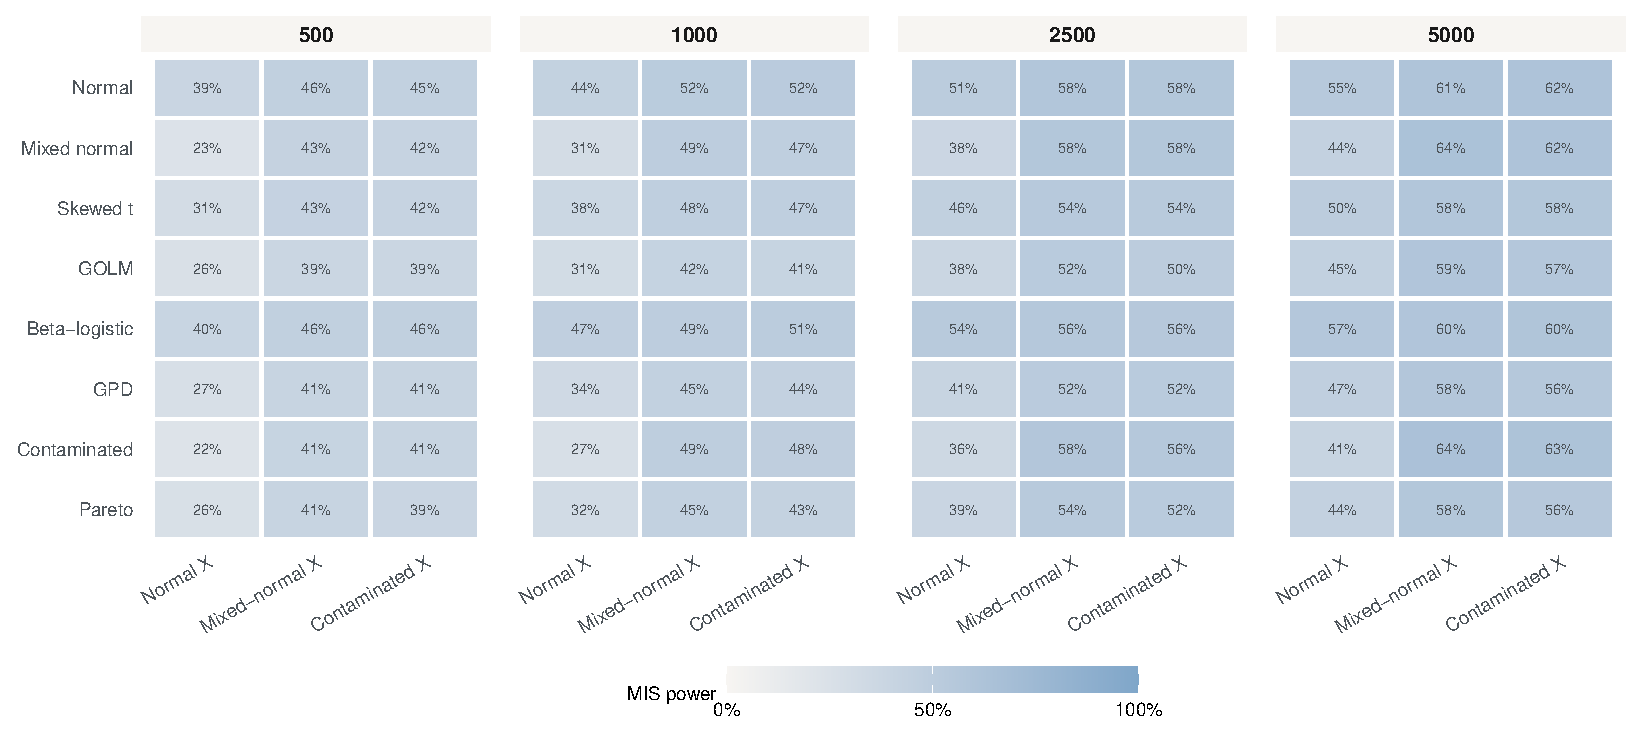
\includegraphics[width=\textwidth]{../../output/05_misspecification/figures/supplement/05_figS05_environment_heterogeneity.pdf}
	\caption{MIS power across predictor distributions, error distributions, and sample sizes in the detailed environment comparison.}
	\label{fig:05S-environment-heterogeneity}
\end{figure}

\begin{table}[htbp]
\centering
\caption{Distribution of MIS power across the 96 environments at each scenario's maximum simulated severity, k/n = 2.5 percent.}
\label{tab:05-worst-case-environment}
\resizebox{0.85\columnwidth}{!}{%
\begin{tabular}{@{}lrrrr@{}}
\toprule
Scenario & Minimum & 10th percentile & Median & Maximum \\
\midrule
Linear endogeneity & 2.4\% & 3.8\% & 5.0\% & 8.0\% \\
Nonlinear confounding & 100.0\% & 100.0\% & 100.0\% & 100.0\% \\
Heterogeneous slope & 96.0\% & 100.0\% & 100.0\% & 100.0\% \\
Heteroskedasticity & 20.6\% & 39.2\% & 98.1\% & 100.0\% \\
Missing interaction & 45.0\% & 99.5\% & 100.0\% & 100.0\% \\
Nonlinearity & 100.0\% & 100.0\% & 100.0\% & 100.0\% \\
Omitted variable & 0.0\% & 0.2\% & 7.2\% & 100.0\% \\
Threshold & 95.4\% & 100.0\% & 100.0\% & 100.0\% \\
\bottomrule
\end{tabular}%
}
\end{table}


The comparison with the classical observation-level diagnostics shows a similar pattern of non-nested rejection sets. MIS-only rejection is common for several nonlinear and heterogeneous mechanisms, while Cook's distance, DFBETAS, and leverage retain some exclusive detections (\autoref{fig:05S-exclusive-classical}). These results reinforce the interpretation of the methods as diagnostics with different targets rather than interchangeable specification tests.

\begin{figure}[htbp]
	\centering
	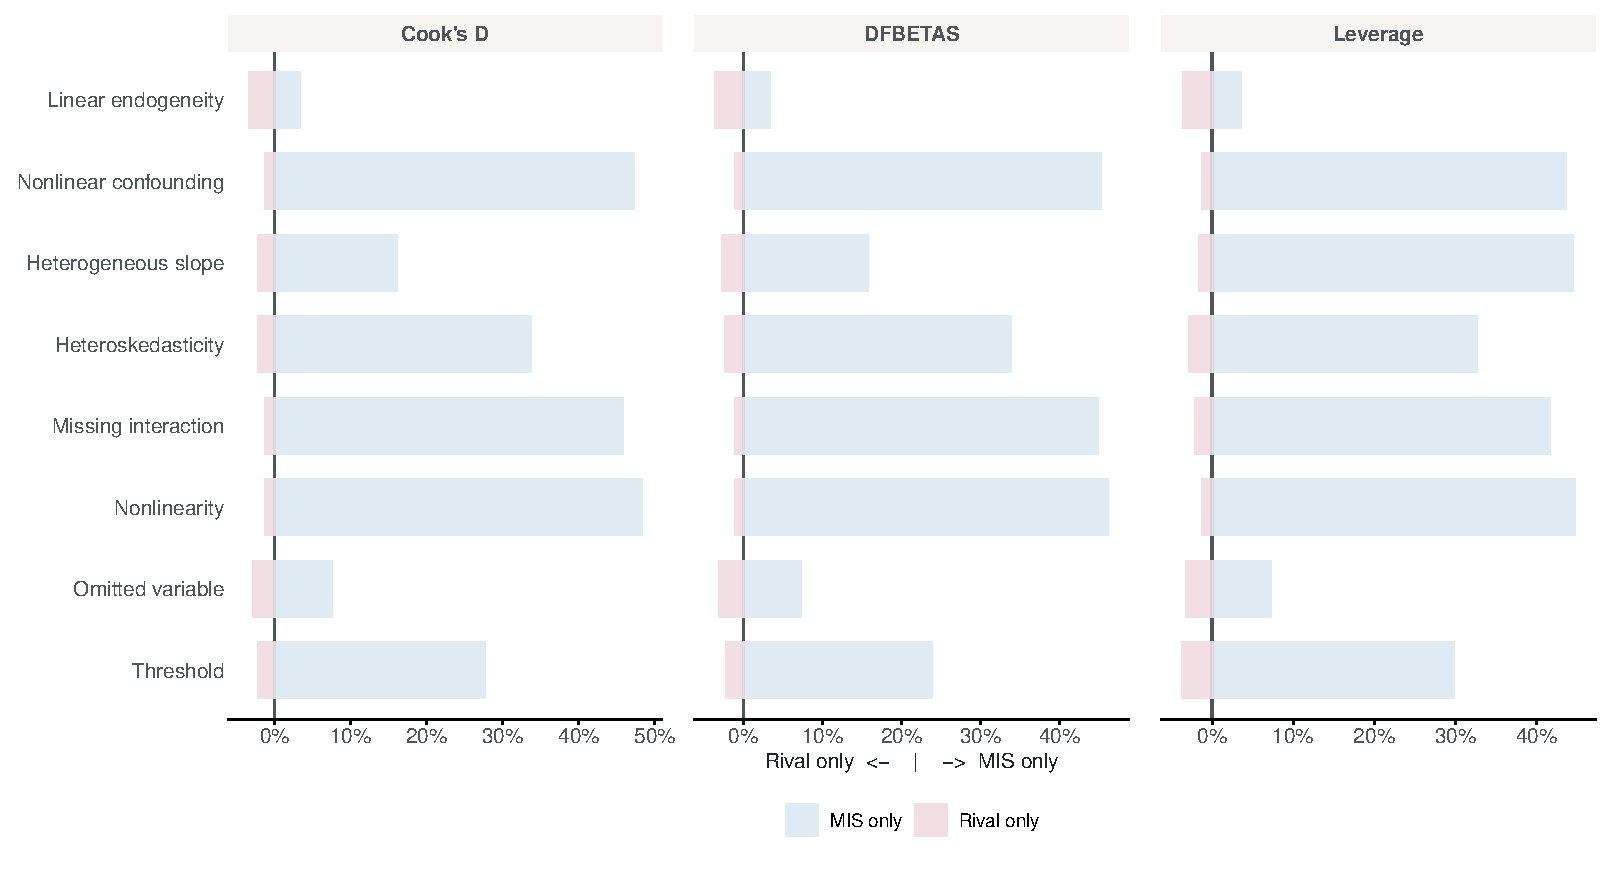
\includegraphics[width=\textwidth]{../../output/05_misspecification/figures/supplement/05_figS04_exclusive_classical.pdf}
	\caption{Exclusive rejection probabilities for MIS relative to Cook's distance, DFBETAS, and leverage at \(k/n=0.025\).}
	\label{fig:05S-exclusive-classical}
\end{figure}

\subsubsection{Boundary and Deletion-Budget Diagnostics}
\label{app:misspec-boundary}

The faceted boundary results provide the complete sample-size pattern underlying \autoref{fig:05-boundary-by-n}. For nonlinear confounding, heterogeneous slopes, missing interactions, nonlinearity, and threshold behaviour, the censoring-aware median boundary declines as sample size increases. Heteroskedasticity also becomes detectable after the smallest design but retains a higher boundary. Linear endogeneity and omitted-variable misspecification remain right-censored throughout the displayed sample-size grid.

\begin{figure}[htbp]
	\centering
	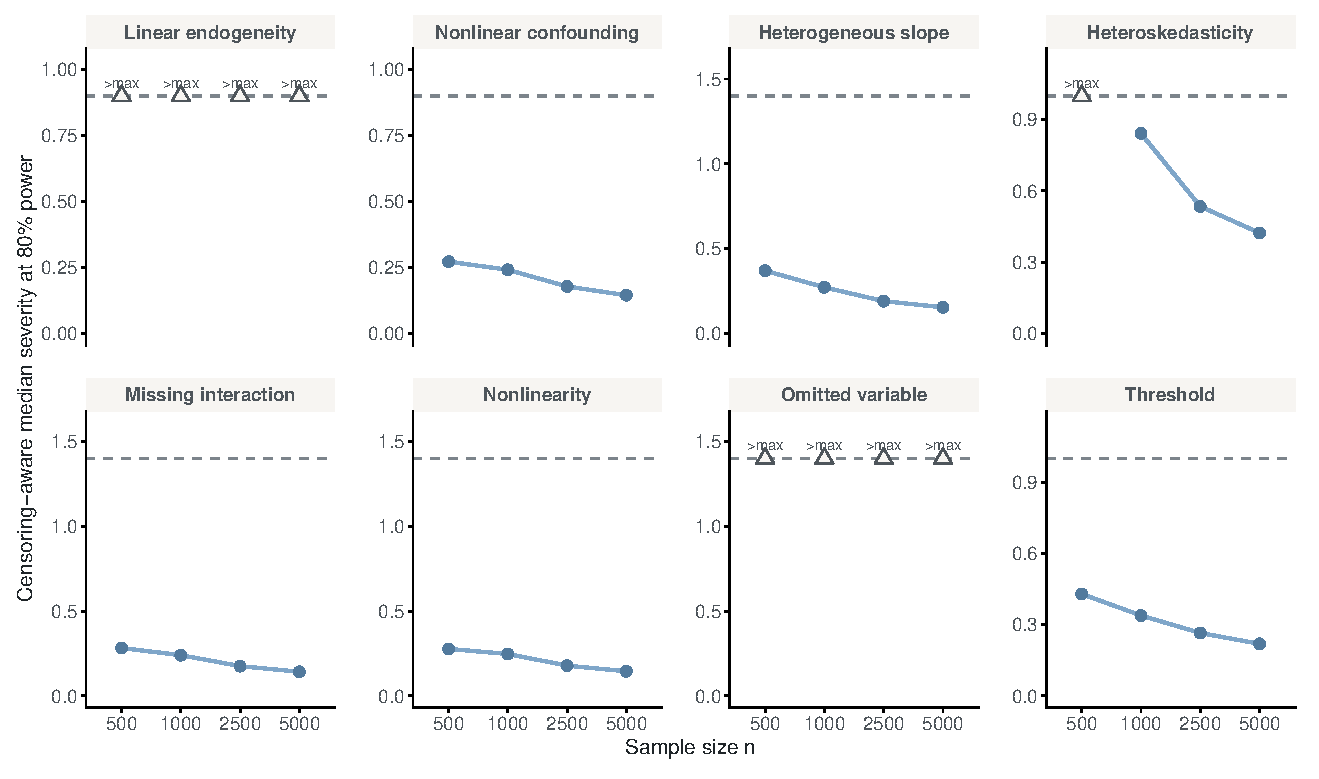
\includegraphics[width=\textwidth]{../../output/05_misspecification/figures/supplement/05_figS06_boundary_by_n_faceted.pdf}
	\caption{Scenario-specific censoring-aware MIS detection boundaries by sample size at \(k/n=0.025\).}
	\label{fig:05S-boundary-faceted}
\end{figure}

\begin{table}[htbp]
\centering
\caption{Boundary censoring audit at k/n = 2.5 percent. Reacher-only means and medians condition on the 80-percent crossing being observed; the censored median retains the non-reaching environments.}
\label{tab:05-boundary-mean}
\resizebox{\columnwidth}{!}{%
\begin{tabular}{@{}lrrrrrr@{}}
\toprule
Scenario & Reachers / 96 & Censored & Reach rate & Censoring-aware median & Reacher mean & Reacher median \\
\midrule
Linear endogeneity & 0 / 96 & 96 & 0.0\% & >0.900 & -- & -- \\
Nonlinear confounding & 96 / 96 & 0 & 100.0\% & 0.200 & 0.224 & 0.200 \\
Heterogeneous slope & 96 / 96 & 0 & 100.0\% & 0.273 & 0.338 & 0.273 \\
Heteroskedasticity & 68 / 96 & 28 & 70.8\% & 0.680 & 0.537 & 0.529 \\
Missing interaction & 91 / 96 & 5 & 94.8\% & 0.253 & 0.322 & 0.246 \\
Nonlinearity & 96 / 96 & 0 & 100.0\% & 0.209 & 0.231 & 0.209 \\
Omitted variable & 8 / 96 & 88 & 8.3\% & >1.400 & 1.029 & 0.951 \\
Threshold & 96 / 96 & 0 & 100.0\% & 0.307 & 0.347 & 0.307 \\
\bottomrule
\end{tabular}%
}
\end{table}


The detailed deletion-budget results show that the pooled operating characteristic does not imply a universally preferred \(k\). For example, missing-interaction reach rises from \(84.4\%\) at \(k/n=0.01\) to \(100.0\%\) at \(0.05\), whereas nonlinear-confounding and heterogeneous-slope reach declines at the \(10\%\) budget. Linear endogeneity remains undetected at every budget, and omitted-variable reach remains low even though it increases to \(19.8\%\) at \(10\%\). The fixed-\(k\) analysis therefore describes sensitivity to analyst-chosen budgets rather than recovery of a latent contamination proportion.

\begin{table}[htbp]
\centering
\caption{MIS deletion-budget sensitivity by scenario.}
\label{tab:05-budget-by-scenario}
\resizebox{0.85\columnwidth}{!}{%
\begin{tabular}{@{}lrrrr@{}}
\toprule
Scenario & k/n & Reachers / 96 & Censored & Censoring-aware median \\
\midrule
Linear endogeneity & 1.0\% & 0 / 96 & 96 & >0.900 \\
Linear endogeneity & 2.5\% & 0 / 96 & 96 & >0.900 \\
Linear endogeneity & 5.0\% & 0 / 96 & 96 & >0.900 \\
Linear endogeneity & 10.0\% & 0 / 96 & 96 & >0.900 \\
\addlinespace
Nonlinear confounding & 1.0\% & 96 / 96 & 0 & 0.188 \\
Nonlinear confounding & 2.5\% & 96 / 96 & 0 & 0.200 \\
Nonlinear confounding & 5.0\% & 96 / 96 & 0 & 0.289 \\
Nonlinear confounding & 10.0\% & 64 / 96 & 32 & 0.534 \\
\addlinespace
Heterogeneous slope & 1.0\% & 89 / 96 & 7 & 0.282 \\
Heterogeneous slope & 2.5\% & 96 / 96 & 0 & 0.273 \\
Heterogeneous slope & 5.0\% & 96 / 96 & 0 & 0.371 \\
Heterogeneous slope & 10.0\% & 64 / 96 & 32 & 0.580 \\
\addlinespace
Heteroskedasticity & 1.0\% & 60 / 96 & 36 & 0.770 \\
Heteroskedasticity & 2.5\% & 68 / 96 & 28 & 0.680 \\
Heteroskedasticity & 5.0\% & 61 / 96 & 35 & 0.710 \\
Heteroskedasticity & 10.0\% & 44 / 96 & 52 & >1.000 \\
\addlinespace
Missing interaction & 1.0\% & 81 / 96 & 15 & 0.240 \\
Missing interaction & 2.5\% & 91 / 96 & 5 & 0.253 \\
Missing interaction & 5.0\% & 96 / 96 & 0 & 0.311 \\
Missing interaction & 10.0\% & 93 / 96 & 3 & 0.422 \\
\addlinespace
Nonlinearity & 1.0\% & 96 / 96 & 0 & 0.190 \\
Nonlinearity & 2.5\% & 96 / 96 & 0 & 0.209 \\
Nonlinearity & 5.0\% & 96 / 96 & 0 & 0.300 \\
Nonlinearity & 10.0\% & 64 / 96 & 32 & 0.596 \\
\addlinespace
Omitted variable & 1.0\% & 4 / 96 & 92 & >1.400 \\
Omitted variable & 2.5\% & 8 / 96 & 88 & >1.400 \\
Omitted variable & 5.0\% & 8 / 96 & 88 & >1.400 \\
Omitted variable & 10.0\% & 19 / 96 & 77 & >1.400 \\
\addlinespace
Threshold & 1.0\% & 88 / 96 & 8 & 0.312 \\
Threshold & 2.5\% & 96 / 96 & 0 & 0.307 \\
Threshold & 5.0\% & 90 / 96 & 6 & 0.434 \\
Threshold & 10.0\% & 53 / 96 & 43 & 0.779 \\
\bottomrule
\end{tabular}%
}
\par\smallskip
\begin{minipage}{0.96\linewidth}
\footnotesize
\textit{Note:} Boundaries are right-censored at the maximum simulated severity, so the censoring-aware median is reported; it is identified whenever fewer than half of environments are censored. Reacher-only means and medians, together with the censoring counts, are given in Table~\ref{tab:05-budget-mean}.
\end{minipage}
\end{table}


\begin{table}[htbp]
\centering
\caption{Deletion-budget boundary audit. Reacher-only means and medians condition on successful detection; censoring counts show the conditioning set explicitly for every scenario and k.}
\label{tab:05-budget-mean}
\resizebox{\columnwidth}{!}{%
\begin{tabular}{@{}lrrrrrrr@{}}
\toprule
Scenario & k/n & Reachers / 96 & Censored & Reach rate & Censoring-aware median & Reacher mean & Reacher median \\
\midrule
Linear endogeneity & 1.0\% & 0 / 96 & 96 & 0.0\% & >0.900 & -- & -- \\
Linear endogeneity & 2.5\% & 0 / 96 & 96 & 0.0\% & >0.900 & -- & -- \\
Linear endogeneity & 5.0\% & 0 / 96 & 96 & 0.0\% & >0.900 & -- & -- \\
Linear endogeneity & 10.0\% & 0 / 96 & 96 & 0.0\% & >0.900 & -- & -- \\
\addlinespace
Nonlinear confounding & 1.0\% & 96 / 96 & 0 & 100.0\% & 0.188 & 0.242 & 0.188 \\
Nonlinear confounding & 2.5\% & 96 / 96 & 0 & 100.0\% & 0.200 & 0.224 & 0.200 \\
Nonlinear confounding & 5.0\% & 96 / 96 & 0 & 100.0\% & 0.289 & 0.323 & 0.289 \\
Nonlinear confounding & 10.0\% & 64 / 96 & 32 & 66.7\% & 0.534 & 0.390 & 0.380 \\
\addlinespace
Heterogeneous slope & 1.0\% & 89 / 96 & 7 & 92.7\% & 0.282 & 0.382 & 0.275 \\
Heterogeneous slope & 2.5\% & 96 / 96 & 0 & 100.0\% & 0.273 & 0.338 & 0.273 \\
Heterogeneous slope & 5.0\% & 96 / 96 & 0 & 100.0\% & 0.371 & 0.385 & 0.371 \\
Heterogeneous slope & 10.0\% & 64 / 96 & 32 & 66.7\% & 0.580 & 0.489 & 0.430 \\
\addlinespace
Heteroskedasticity & 1.0\% & 60 / 96 & 36 & 62.5\% & 0.770 & 0.555 & 0.550 \\
Heteroskedasticity & 2.5\% & 68 / 96 & 28 & 70.8\% & 0.680 & 0.537 & 0.529 \\
Heteroskedasticity & 5.0\% & 61 / 96 & 35 & 63.5\% & 0.710 & 0.540 & 0.550 \\
Heteroskedasticity & 10.0\% & 44 / 96 & 52 & 45.8\% & >1.000 & 0.628 & 0.645 \\
\addlinespace
Missing interaction & 1.0\% & 81 / 96 & 15 & 84.4\% & 0.240 & 0.309 & 0.198 \\
Missing interaction & 2.5\% & 91 / 96 & 5 & 94.8\% & 0.253 & 0.322 & 0.246 \\
Missing interaction & 5.0\% & 96 / 96 & 0 & 100.0\% & 0.311 & 0.357 & 0.311 \\
Missing interaction & 10.0\% & 93 / 96 & 3 & 96.9\% & 0.422 & 0.493 & 0.414 \\
\addlinespace
Nonlinearity & 1.0\% & 96 / 96 & 0 & 100.0\% & 0.190 & 0.268 & 0.190 \\
Nonlinearity & 2.5\% & 96 / 96 & 0 & 100.0\% & 0.209 & 0.231 & 0.209 \\
Nonlinearity & 5.0\% & 96 / 96 & 0 & 100.0\% & 0.300 & 0.355 & 0.300 \\
Nonlinearity & 10.0\% & 64 / 96 & 32 & 66.7\% & 0.596 & 0.464 & 0.390 \\
\addlinespace
Omitted variable & 1.0\% & 4 / 96 & 92 & 4.2\% & >1.400 & 1.222 & 1.203 \\
Omitted variable & 2.5\% & 8 / 96 & 88 & 8.3\% & >1.400 & 1.029 & 0.951 \\
Omitted variable & 5.0\% & 8 / 96 & 88 & 8.3\% & >1.400 & 0.951 & 0.936 \\
Omitted variable & 10.0\% & 19 / 96 & 77 & 19.8\% & >1.400 & 0.750 & 0.673 \\
\addlinespace
Threshold & 1.0\% & 88 / 96 & 8 & 91.7\% & 0.312 & 0.355 & 0.299 \\
Threshold & 2.5\% & 96 / 96 & 0 & 100.0\% & 0.307 & 0.347 & 0.307 \\
Threshold & 5.0\% & 90 / 96 & 6 & 93.8\% & 0.434 & 0.434 & 0.415 \\
Threshold & 10.0\% & 53 / 96 & 43 & 55.2\% & 0.779 & 0.424 & 0.402 \\
\bottomrule
\end{tabular}%
}
\end{table}


\subsubsection{Correct-Model Calibration and Supplementary Estimation}
\label{app:misspec-estimation}

The corrected-model cutoff audit confirms that the respecified-model analysis uses finite independently calibrated cutoffs in every recorded model class (\autoref{tab:05-correct-cutoff-audit}). Together with the approximately \(5\%\) corrected-model rejection rates in the main text, this supports the interpretation of the specificity exercise as a calibrated comparison rather than a mechanical consequence of reusing wrong-model thresholds.

\begin{table}[htbp]
\centering
\caption{Correct-model MIS null cutoffs from the independent 05c calibration at k/n = 2.5 percent.}
\label{tab:05-correct-cutoff-audit}
\resizebox{0.85\columnwidth}{!}{%
\begin{tabular}{@{}lrrrr@{}}
\toprule
Correct model class & Median cutoff & 10th percentile & 90th percentile & Finite rate \\
\midrule
Heterogeneous slope & 7.040 & 3.380 & 12.580 & 100.0\% \\
Missing interaction & 5.623 & 3.209 & 9.271 & 100.0\% \\
Nonlinearity & 6.675 & 3.213 & 11.562 & 100.0\% \\
Omitted variable & 5.226 & 3.202 & 8.508 & 100.0\% \\
Threshold & 9.262 & 3.393 & 20.998 & 100.0\% \\
\bottomrule
\end{tabular}%
}
\end{table}


The frozen-05 estimation results address a different question from the formal detection experiment. When the missing model structure is explicitly restored, full-MM estimation has small absolute bias and coverage close to \(95\%\) across the recorded corrected-model cases (\autoref{tab:05-frozen-mm-correct-wrong}). Under the corresponding wrong models, bias and coverage can deteriorate substantially. These results concern estimation under corrected and incorrect specifications and should not be interpreted as evidence that deleting MIS-selected observations performs the same correction.

\begin{table}[htbp]
\centering
\caption{Frozen-05 full-MM estimation under wrong and correctly respecified models, reported separately by X distribution.}
\label{tab:05-frozen-mm-correct-wrong}
\resizebox{\columnwidth}{!}{%
\begin{tabular}{@{}lllrrrrr@{}}
\toprule
X distribution & Scenario & State & Abs. bias & RMSE & Coverage & SE ratio & Predicted coverage \\
\midrule
Normal X & Heterogeneous slope & Correct & 0.019 & 0.024 & 94.9\% & 1.012 & 95.0\% \\
Normal X & Heterogeneous slope & Wrong & 0.260 & 0.264 & 0.0\% & 0.768 & 0.2\% \\
Normal X & Missing interaction & Correct & 0.019 & 0.023 & 94.8\% & 1.009 & 94.8\% \\
Normal X & Missing interaction & Wrong & 0.067 & 0.084 & 81.7\% & 0.694 & 81.7\% \\
Normal X & Nonlinearity & Correct & 0.017 & 0.021 & 94.5\% & 1.004 & 94.8\% \\
Normal X & Nonlinearity & Wrong & 0.090 & 0.114 & 66.9\% & 0.506 & 66.6\% \\
Normal X & Omitted variable & Correct & 0.018 & 0.023 & 95.6\% & 1.025 & 95.3\% \\
Normal X & Omitted variable & Wrong & 0.431 & 0.433 & 0.0\% & 0.909 & 0.0\% \\
Normal X & Structural break & Correct & 0.019 & 0.023 & 95.4\% & 1.012 & 94.8\% \\
Normal X & Structural break & Wrong & 0.259 & 0.262 & 0.1\% & 0.845 & 0.1\% \\
Normal X & Threshold & Correct & 0.023 & 0.029 & 95.1\% & 1.009 & 94.8\% \\
Normal X & Threshold & Wrong & 0.475 & 0.477 & 0.0\% & 0.784 & 0.0\% \\
\addlinespace
Mixed-normal X & Heterogeneous slope & Correct & 0.006 & 0.007 & 95.2\% & 1.017 & 94.9\% \\
Mixed-normal X & Heterogeneous slope & Wrong & 0.023 & 0.025 & 22.8\% & 0.810 & 21.8\% \\
Mixed-normal X & Missing interaction & Correct & 0.006 & 0.007 & 94.8\% & 1.004 & 94.8\% \\
Mixed-normal X & Missing interaction & Wrong & 0.082 & 0.103 & 52.0\% & 0.369 & 52.6\% \\
Mixed-normal X & Nonlinearity & Correct & 0.005 & 0.006 & 95.1\% & 1.021 & 95.0\% \\
Mixed-normal X & Nonlinearity & Wrong & 0.081 & 0.102 & 66.9\% & 0.504 & 66.6\% \\
Mixed-normal X & Omitted variable & Correct & 0.006 & 0.007 & 94.6\% & 0.994 & 94.5\% \\
Mixed-normal X & Omitted variable & Wrong & 0.141 & 0.142 & 0.0\% & 0.698 & 0.1\% \\
Mixed-normal X & Structural break & Correct & 0.006 & 0.007 & 94.6\% & 0.996 & 94.6\% \\
Mixed-normal X & Structural break & Wrong & 0.023 & 0.025 & 23.4\% & 0.806 & 22.6\% \\
Mixed-normal X & Threshold & Correct & 0.007 & 0.009 & 94.8\% & 0.999 & 94.7\% \\
Mixed-normal X & Threshold & Wrong & 0.069 & 0.076 & 2.0\% & 0.417 & 4.6\% \\
\addlinespace
Contaminated X & Heterogeneous slope & Correct & 0.001 & 0.002 & 95.1\% & 0.991 & 94.6\% \\
Contaminated X & Heterogeneous slope & Wrong & 0.002 & 0.003 & 64.8\% & 0.819 & 62.7\% \\
Contaminated X & Missing interaction & Correct & 0.001 & 0.002 & 94.3\% & 1.004 & 94.6\% \\
Contaminated X & Missing interaction & Wrong & 0.112 & 0.139 & 22.4\% & 0.145 & 22.2\% \\
Contaminated X & Nonlinearity & Correct & 0.001 & 0.001 & 93.9\% & 0.975 & 93.8\% \\
Contaminated X & Nonlinearity & Wrong & 0.076 & 0.095 & 68.9\% & 0.532 & 69.0\% \\
Contaminated X & Omitted variable & Correct & 0.001 & 0.002 & 95.1\% & 0.992 & 94.4\% \\
Contaminated X & Omitted variable & Wrong & 0.030 & 0.030 & 0.0\% & 0.712 & 0.0\% \\
Contaminated X & Structural break & Correct & 0.001 & 0.001 & 95.2\% & 1.010 & 94.9\% \\
Contaminated X & Structural break & Wrong & 0.002 & 0.003 & 64.3\% & 0.831 & 61.8\% \\
Contaminated X & Threshold & Correct & 0.002 & 0.002 & 94.7\% & 0.974 & 94.1\% \\
Contaminated X & Threshold & Wrong & 0.026 & 0.039 & 14.1\% & 0.176 & 3.7\% \\
\bottomrule
\end{tabular}%
}
\par\smallskip
\begin{minipage}{0.96\linewidth}
\footnotesize
\textit{Note:} SE ratio is mean reported SE divided by the sampling-SD proxy sqrt(RMSE squared minus mean bias squared); predicted coverage is the corresponding normal approximation.
\end{minipage}
\end{table}


The comparison of full OLS and full MM similarly shows that lower RMSE does not imply improved interval calibration in every environment. MM has lower RMSE in all eight recorded scenarios within each predictor-distribution stratum, but coverage is closer to \(95\%\) in none of the normal-\(X\) cases and in only four of eight cases under each of the mixed-normal and contaminated predictor designs (\autoref{tab:05-frozen-mm-win-counts}).

\begin{table}[htbp]
\centering
\caption{Frozen-05 estimation comparison of full OLS and full MM. Results are reported within X-distribution strata; no comparison of frozen-05 severity values with the formal 05a scale is made.}
\label{tab:05-frozen-ols-vs-mm}
\resizebox{\columnwidth}{!}{%
\begin{tabular}{@{}llrrrrl@{}}
\toprule
X distribution & Scenario & OLS RMSE & MM RMSE & OLS coverage & MM coverage & MM closer to 95 percent \\
\midrule
Normal X & Linear endogeneity & 0.535 & 0.533 & 0.0\% & 0.0\% & No \\
Normal X & Heterogeneous slope & 0.475 & 0.264 & 17.3\% & 0.0\% & No \\
Normal X & Heteroskedasticity & 0.255 & 0.040 & 87.0\% & 86.2\% & No \\
Normal X & Missing interaction & 0.186 & 0.084 & 89.7\% & 81.7\% & No \\
Normal X & Nonlinearity & 0.206 & 0.114 & 77.2\% & 66.9\% & No \\
Normal X & Omitted variable & 0.475 & 0.433 & 17.4\% & 0.0\% & No \\
Normal X & Structural break & 0.469 & 0.262 & 17.6\% & 0.1\% & No \\
Normal X & Threshold & 0.641 & 0.477 & 12.7\% & 0.0\% & No \\
\addlinespace
Mixed-normal X & Linear endogeneity & 0.316 & 0.315 & 0.0\% & 0.0\% & No \\
Mixed-normal X & Heterogeneous slope & 0.146 & 0.025 & 17.9\% & 22.8\% & Yes \\
Mixed-normal X & Heteroskedasticity & 0.102 & 0.033 & 69.4\% & 53.8\% & No \\
Mixed-normal X & Missing interaction & 0.671 & 0.103 & 31.9\% & 52.0\% & Yes \\
Mixed-normal X & Nonlinearity & 3.217 & 0.102 & 22.6\% & 66.9\% & Yes \\
Mixed-normal X & Omitted variable & 0.156 & 0.142 & 16.2\% & 0.0\% & No \\
Mixed-normal X & Structural break & 0.144 & 0.025 & 17.8\% & 23.4\% & Yes \\
Mixed-normal X & Threshold & 0.204 & 0.076 & 12.4\% & 2.0\% & No \\
\addlinespace
Contaminated X & Linear endogeneity & 0.130 & 0.130 & 0.0\% & 0.0\% & No \\
Contaminated X & Heterogeneous slope & 0.031 & 0.003 & 17.9\% & 64.8\% & Yes \\
Contaminated X & Heteroskedasticity & 0.025 & 0.013 & 66.0\% & 43.1\% & No \\
Contaminated X & Missing interaction & 0.762 & 0.139 & 25.7\% & 22.4\% & No \\
Contaminated X & Nonlinearity & 17.313 & 0.095 & 20.4\% & 68.9\% & Yes \\
Contaminated X & Omitted variable & 0.032 & 0.030 & 16.3\% & 0.0\% & No \\
Contaminated X & Structural break & 0.030 & 0.003 & 18.4\% & 64.3\% & Yes \\
Contaminated X & Threshold & 0.042 & 0.039 & 12.2\% & 14.1\% & Yes \\
\bottomrule
\end{tabular}%
}
\end{table}


\begin{table}[htbp]
\centering
\caption{Frozen-05 count of scenarios in which full MM has lower RMSE or coverage closer to 95 percent than full OLS, reported separately by X distribution.}
\label{tab:05-frozen-mm-win-counts}
\resizebox{0.70\columnwidth}{!}{%
\begin{tabular}{@{}lrr@{}}
\toprule
X distribution & MM RMSE wins & MM coverage wins \\
\midrule
Normal X & 8/8 & 0/8 \\
Mixed-normal X & 8/8 & 4/8 \\
Contaminated X & 8/8 & 4/8 \\
\bottomrule
\end{tabular}%
}
\end{table}


Finally, the deletion-arm results show why detection should not be equated with model repair. MIS deletion frequently increases the mean cell-level RMSE as the deletion fraction grows, particularly under mixed-normal and contaminated predictors. With contaminated predictors, for example, mean cell RMSE for MIS deletion rises from \(5.697\) at a \(1\%\) deletion budget to \(18.209\) at \(10\%\), compared with \(2.296\) for the unchanged full OLS fit. The structural defect remains in the estimating model after deletion, so improved diagnostic localisation does not imply improved estimation.

\begin{table}[htbp]
\centering
\caption{Frozen-05 deletion-arm RMSE sensitivity. Arithmetic means and medians of the cell-level RMSE are shown side by side; the severity-0 null cell is excluded and X distributions remain separated.}
\label{tab:05-frozen-rmse-mean-median}
\resizebox{\columnwidth}{!}{%
\begin{tabular}{@{}lllrr@{}}
\toprule
X distribution & k/n & Arm & Mean cell RMSE & Median cell RMSE \\
\midrule
Normal X & 1.0\% & Full OLS & 0.405 & 0.285 \\
Normal X & 1.0\% & MIS deletion & 0.457 & 0.349 \\
Normal X & 1.0\% & Cook deletion & 0.348 & 0.229 \\
Normal X & 1.0\% & DFBETAS deletion & 0.344 & 0.226 \\
Normal X & 1.0\% & Leverage deletion & 0.402 & 0.281 \\
\addlinespace
Normal X & 2.5\% & Full OLS & 0.405 & 0.285 \\
Normal X & 2.5\% & MIS deletion & 0.548 & 0.395 \\
Normal X & 2.5\% & Cook deletion & 0.328 & 0.216 \\
Normal X & 2.5\% & DFBETAS deletion & 0.324 & 0.214 \\
Normal X & 2.5\% & Leverage deletion & 0.402 & 0.283 \\
\addlinespace
Normal X & 5.0\% & Full OLS & 0.405 & 0.285 \\
Normal X & 5.0\% & MIS deletion & 0.654 & 0.425 \\
Normal X & 5.0\% & Cook deletion & 0.310 & 0.201 \\
Normal X & 5.0\% & DFBETAS deletion & 0.307 & 0.202 \\
Normal X & 5.0\% & Leverage deletion & 0.403 & 0.287 \\
\addlinespace
Normal X & 10.0\% & Full OLS & 0.405 & 0.285 \\
Normal X & 10.0\% & MIS deletion & 0.882 & 0.550 \\
Normal X & 10.0\% & Cook deletion & 0.295 & 0.194 \\
Normal X & 10.0\% & DFBETAS deletion & 0.298 & 0.205 \\
Normal X & 10.0\% & Leverage deletion & 0.406 & 0.287 \\
\addlinespace
Mixed-normal X & 1.0\% & Full OLS & 0.619 & 0.182 \\
Mixed-normal X & 1.0\% & MIS deletion & 1.309 & 0.186 \\
Mixed-normal X & 1.0\% & Cook deletion & 0.485 & 0.134 \\
Mixed-normal X & 1.0\% & DFBETAS deletion & 0.485 & 0.133 \\
Mixed-normal X & 1.0\% & Leverage deletion & 0.404 & 0.173 \\
\addlinespace
Mixed-normal X & 2.5\% & Full OLS & 0.619 & 0.182 \\
Mixed-normal X & 2.5\% & MIS deletion & 2.062 & 0.376 \\
Mixed-normal X & 2.5\% & Cook deletion & 0.435 & 0.129 \\
Mixed-normal X & 2.5\% & DFBETAS deletion & 0.432 & 0.129 \\
Mixed-normal X & 2.5\% & Leverage deletion & 0.330 & 0.173 \\
\addlinespace
Mixed-normal X & 5.0\% & Full OLS & 0.619 & 0.182 \\
Mixed-normal X & 5.0\% & MIS deletion & 2.591 & 0.533 \\
Mixed-normal X & 5.0\% & Cook deletion & 0.353 & 0.126 \\
Mixed-normal X & 5.0\% & DFBETAS deletion & 0.343 & 0.132 \\
Mixed-normal X & 5.0\% & Leverage deletion & 0.251 & 0.164 \\
\addlinespace
Mixed-normal X & 10.0\% & Full OLS & 0.619 & 0.182 \\
Mixed-normal X & 10.0\% & MIS deletion & 3.198 & 0.667 \\
Mixed-normal X & 10.0\% & Cook deletion & 0.284 & 0.127 \\
Mixed-normal X & 10.0\% & DFBETAS deletion & 0.237 & 0.127 \\
Mixed-normal X & 10.0\% & Leverage deletion & 0.221 & 0.136 \\
\addlinespace
Contaminated X & 1.0\% & Full OLS & 2.296 & 0.043 \\
Contaminated X & 1.0\% & MIS deletion & 5.697 & 0.044 \\
Contaminated X & 1.0\% & Cook deletion & 1.923 & 0.030 \\
Contaminated X & 1.0\% & DFBETAS deletion & 1.926 & 0.029 \\
Contaminated X & 1.0\% & Leverage deletion & 1.346 & 0.046 \\
\addlinespace
Contaminated X & 2.5\% & Full OLS & 2.296 & 0.043 \\
Contaminated X & 2.5\% & MIS deletion & 9.105 & 0.093 \\
Contaminated X & 2.5\% & Cook deletion & 1.988 & 0.029 \\
Contaminated X & 2.5\% & DFBETAS deletion & 1.968 & 0.029 \\
Contaminated X & 2.5\% & Leverage deletion & 1.055 & 0.050 \\
\addlinespace
Contaminated X & 5.0\% & Full OLS & 2.296 & 0.043 \\
Contaminated X & 5.0\% & MIS deletion & 11.977 & 0.162 \\
Contaminated X & 5.0\% & Cook deletion & 2.086 & 0.029 \\
Contaminated X & 5.0\% & DFBETAS deletion & 2.028 & 0.032 \\
Contaminated X & 5.0\% & Leverage deletion & 0.763 & 0.058 \\
\addlinespace
Contaminated X & 10.0\% & Full OLS & 2.296 & 0.043 \\
Contaminated X & 10.0\% & MIS deletion & 18.209 & 0.393 \\
Contaminated X & 10.0\% & Cook deletion & 2.049 & 0.030 \\
Contaminated X & 10.0\% & DFBETAS deletion & 1.115 & 0.041 \\
Contaminated X & 10.0\% & Leverage deletion & 0.175 & 0.074 \\
\bottomrule
\end{tabular}%
}
\end{table}











	
\end{document}
